\documentclass[10pt, compress, aspectratio=169]{beamer}

\usetheme[numbering=fraction, progressbar=none, titleformat=smallcaps]{metropolis}
\usepackage{booktabs}
\usepackage{array}
\usepackage{listings}
\usepackage{graphicx}
\usepackage[scale=2]{ccicons}
\usepackage{url}
\usepackage{relsize}
\usepackage{wasysym}

\usepackage{pgfplots}
\usepgfplotslibrary{dateplot}

\lstset{ %
  backgroundcolor={},
  basicstyle=\ttfamily\footnotesize,
  breakatwhitespace=true,
  breaklines=true,
  captionpos=n,
  commentstyle=\color{orange},
  escapeinside={\%*}{*)},
  extendedchars=true,
  frame=n,
  keywordstyle=\color{orange},
  language=bash,
  rulecolor=\color{black},
  showspaces=false,
  showstringspaces=false,
  showtabs=false,
  numbers=left,
  numbersep=3pt,
  stepnumber=1,
  stringstyle=\color{gray},
  tabsize=2,
  keywords={thrust,plus,device_vector, copy,transform,begin,end, copyin,
  copyout, acc, \_\_global\_\_, void, int, float, main, threadIdx, blockIdx,
  blockDim, if, else, malloc, NULL, cudaMalloc, cudaMemcpy, cudaSuccess,
  cudaGetLastError, cudaDeviceSynchronize, cudaFree, cudaMemcpyDeviceToHost,
  cudaMemcpyHostToDevice, const, data, independent, kernels, loop,
  fprintf, stderr, cudaGetErrorString, EXIT_FAILURE, for, dim3},
  otherkeywords={::, \#pragma, \#include, <<<,>>>, \&, \*, +, -, /, [, ], >, <}
}

\renewcommand*{\UrlFont}{\ttfamily\smaller\relax}

\graphicspath{{images/}}

\title{From linuxdev-br to GSoC: Kernel Virtual Displays}
\author{\footnotesize Rodrigo Siqueira \\ {\scriptsize rodrigosiqueiramelo@gmail.com} \\ {\scriptsize \url{http://siqueira.tech}} }
\institute{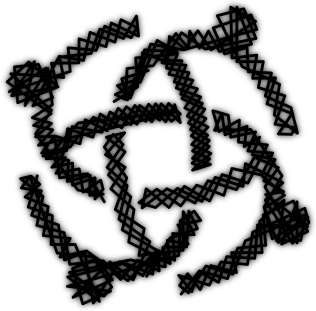
\includegraphics[height=2cm]{linuxdev-br_logo}\\[0.2cm]}

\begin{document}

\maketitle

%------------------------------------------------------------------------------
\section{Journey to the Center of the Direct Rendering Manager}

\section{1000000 foot view}
\begin{frame}{1000000 foot view}
  \metroset{block=fill}
  \begin{exampleblock}{Cards}
    \begin{itemize}
      \item Integrated Graphics \pause
      \item Dedicated Graphics \pause
      \item GPU Switching \pause
    \end{itemize}
  \end{exampleblock}

  \metroset{block=fill}
  \begin{exampleblock}{Framebuffer}
    Modes \pause
    \begin{itemize}
      \item Display Resolution \pause
      \item Color Depth \pause
      \item Refresh Rate
    \end{itemize}
  \end{exampleblock}

\end{frame}

\section{100000 foot view}
\begin{frame}{100000 foot view}
  \begin{figure}
    \centering
    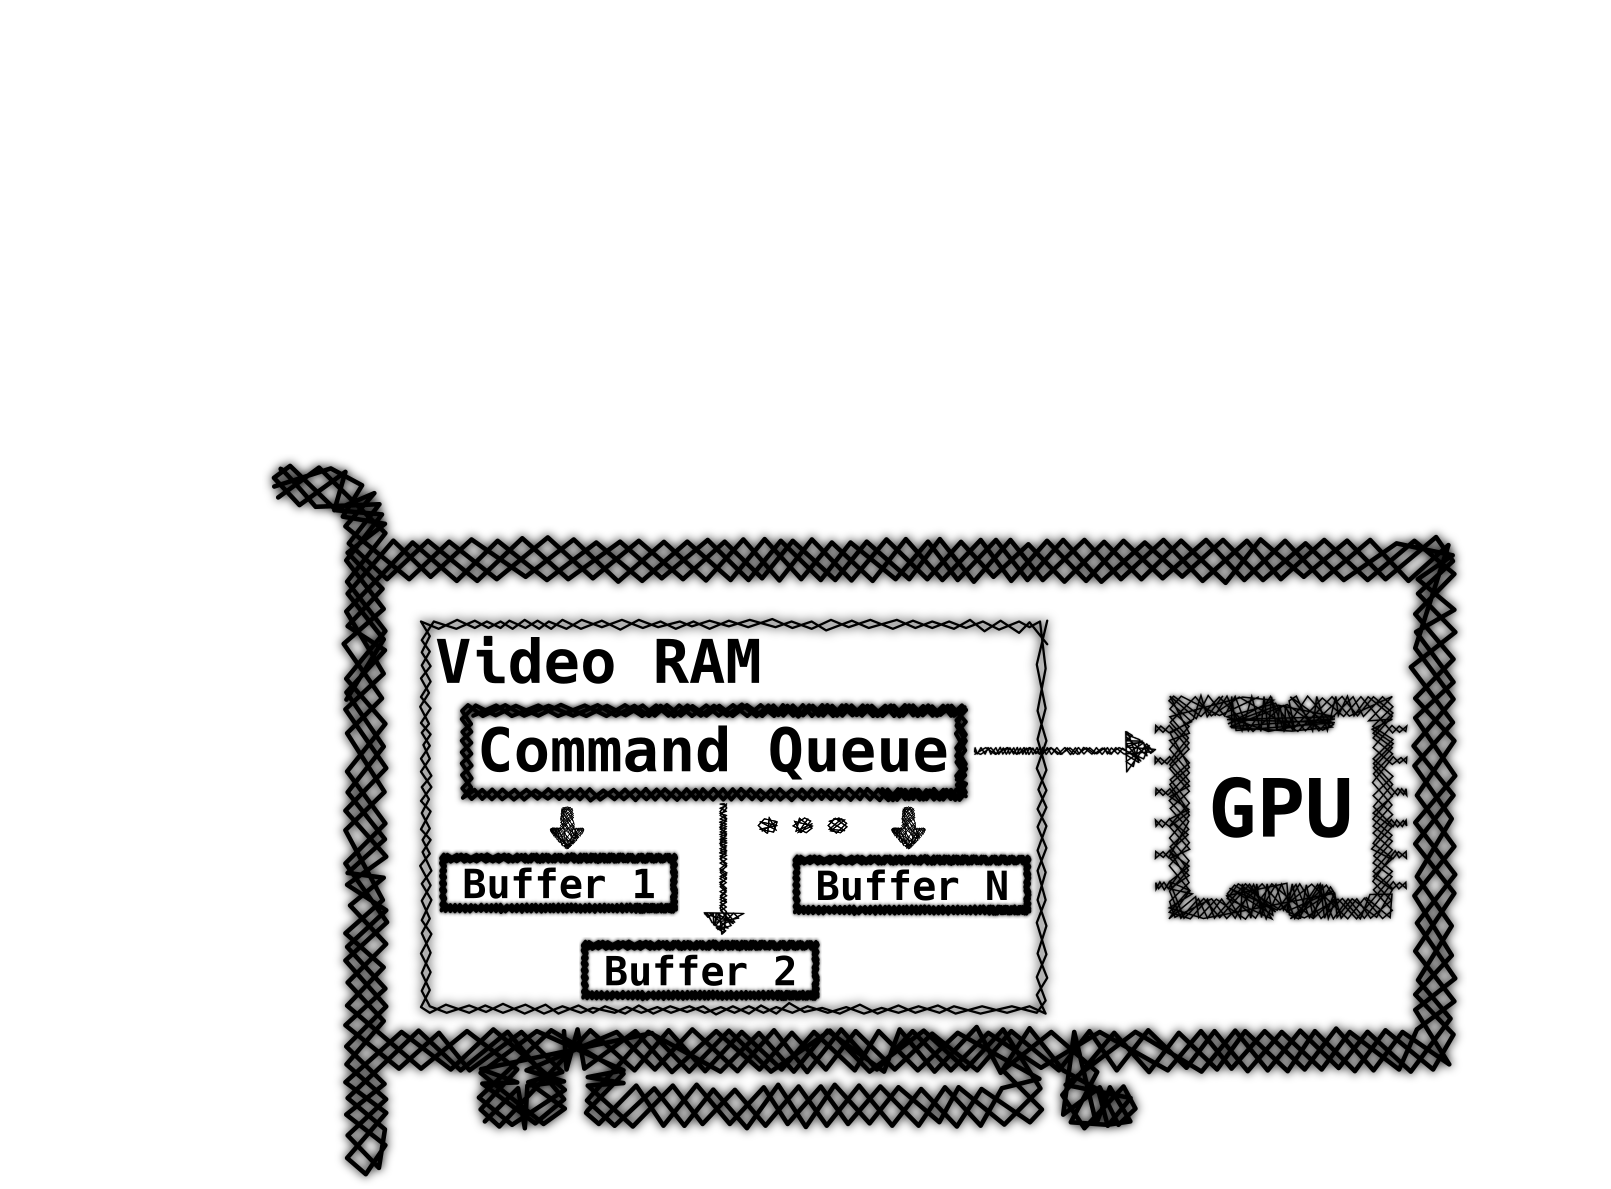
\includegraphics[width=\linewidth,
                     height=0.8\textheight,
                     keepaspectratio]{no_drm_1}
  \end{figure}
\end{frame}

\begin{frame}{100000 foot view}
  \begin{figure}
    \centering
    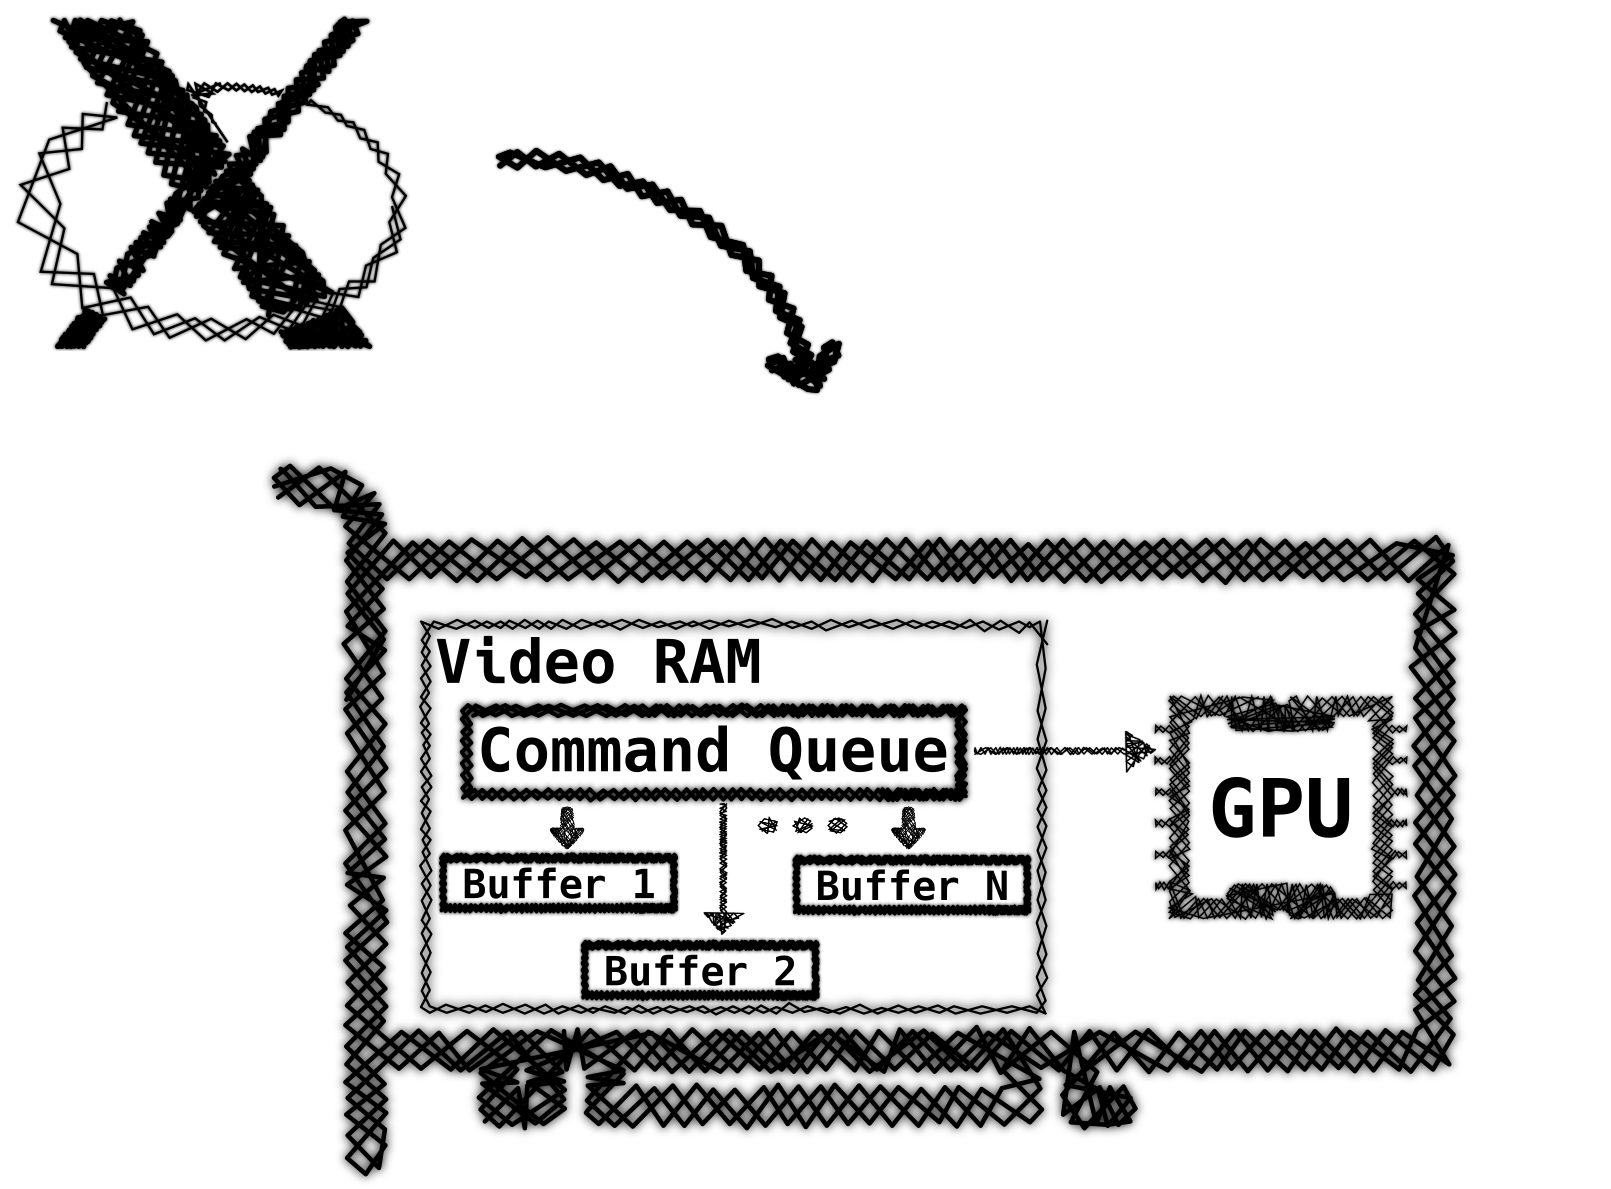
\includegraphics[width=\linewidth,
                     height=0.8\textheight,
                     keepaspectratio]{no_drm_2}
  \end{figure}
\end{frame}

\begin{frame}{100000 foot view}
  \begin{figure}
    \centering
    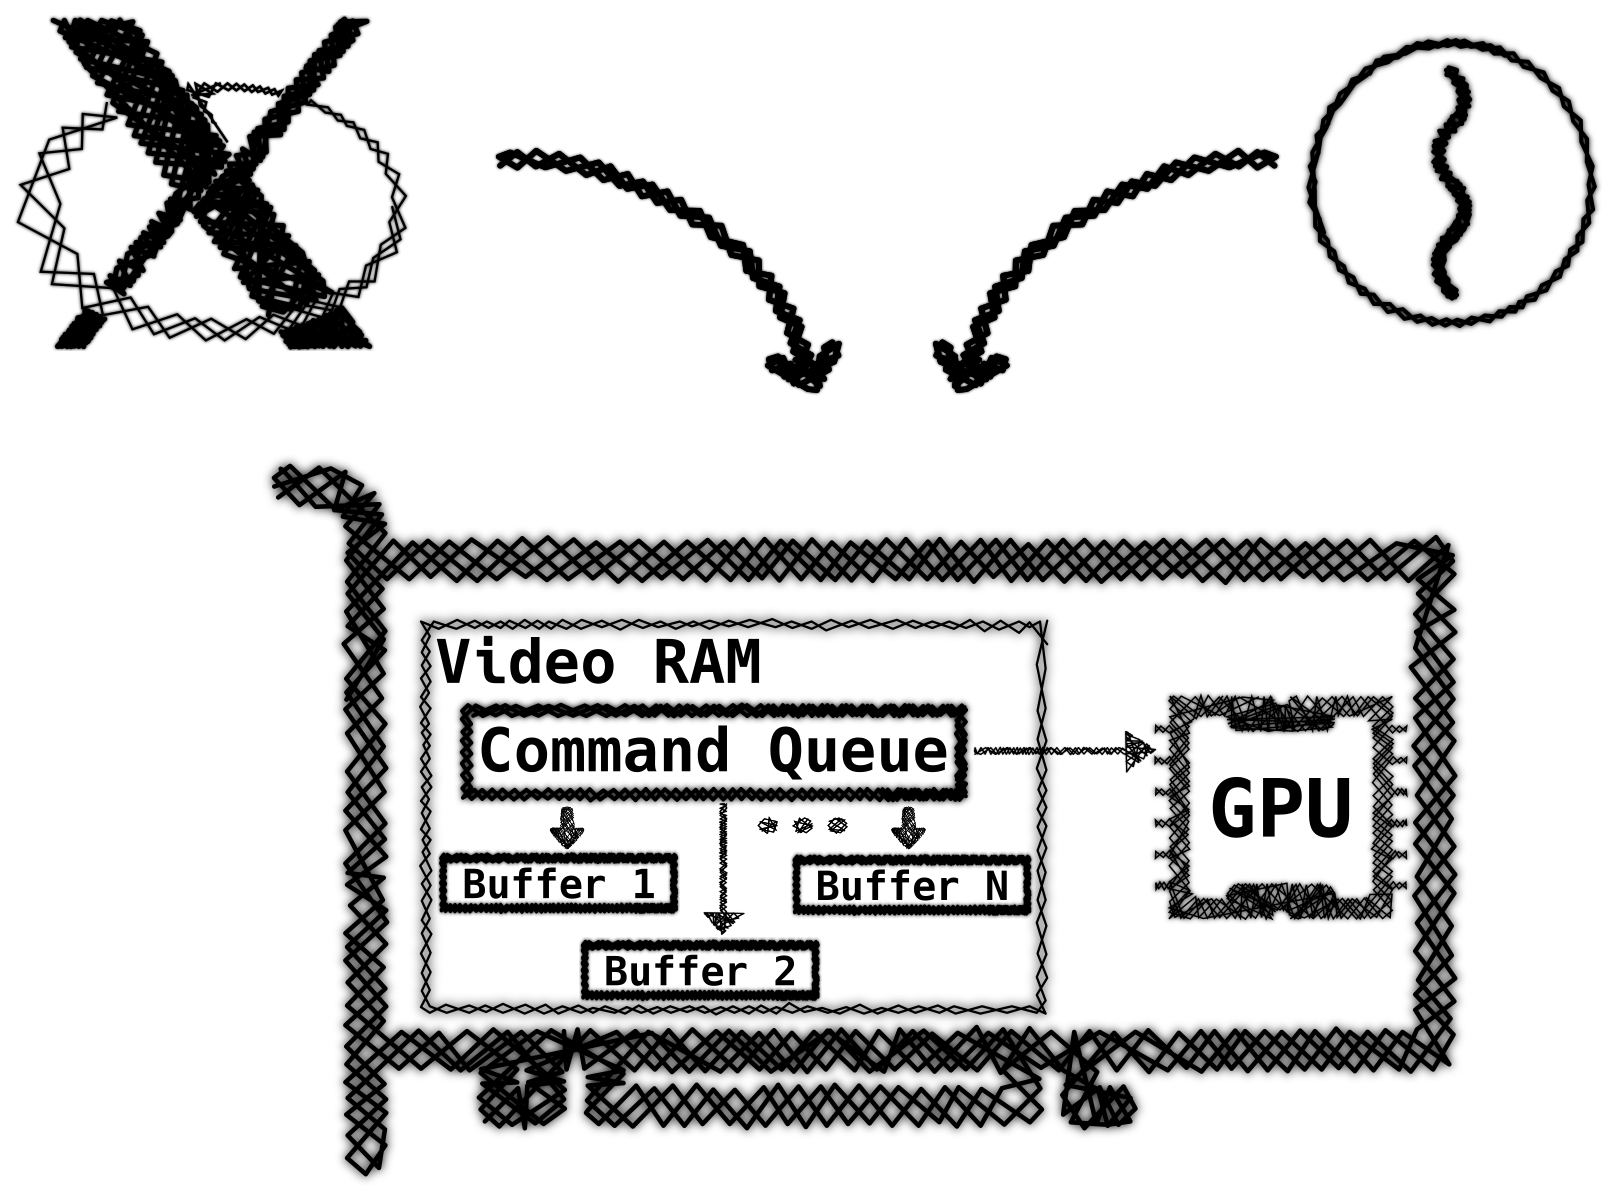
\includegraphics[width=\linewidth,
                     height=0.8\textheight,
                     keepaspectratio]{no_drm_3}
  \end{figure}
\end{frame}

\begin{frame}{100000 foot view}
  \begin{figure}
    \centering
    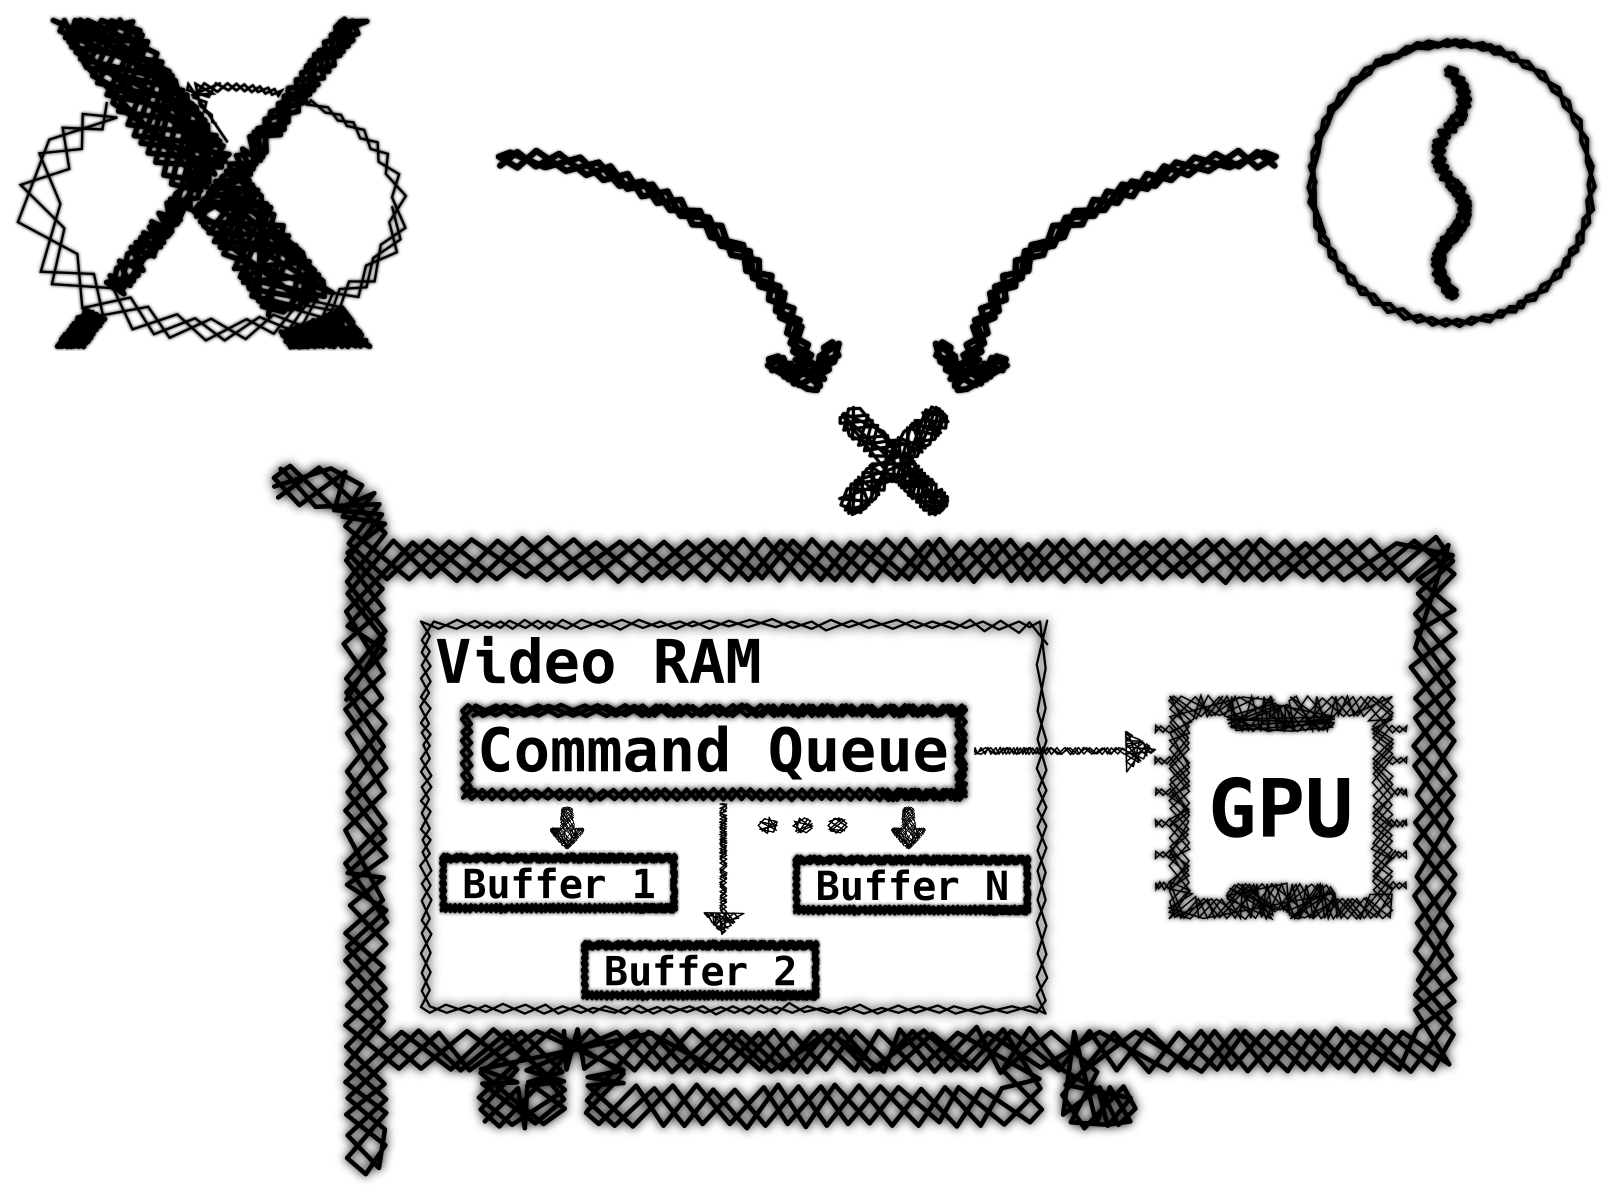
\includegraphics[width=\linewidth,
                     height=0.8\textheight,
                     keepaspectratio]{no_drm}
  \end{figure}
\end{frame}

\begin{frame}{100000 foot view}
  \metroset{block=fill}
  \begin{exampleblock}{Problems}
    \begin{itemize}
      \item Code duplication (DDX Vs. fbdev) \pause
      \item Mix between User and Kernel Space \pause
      \item Management problems \pause
    \end{itemize}
  \end{exampleblock}
\end{frame}

%------------------------------------------------------------------------------
\begin{frame}{100000 foot view}
  \begin{figure}
    \centering
    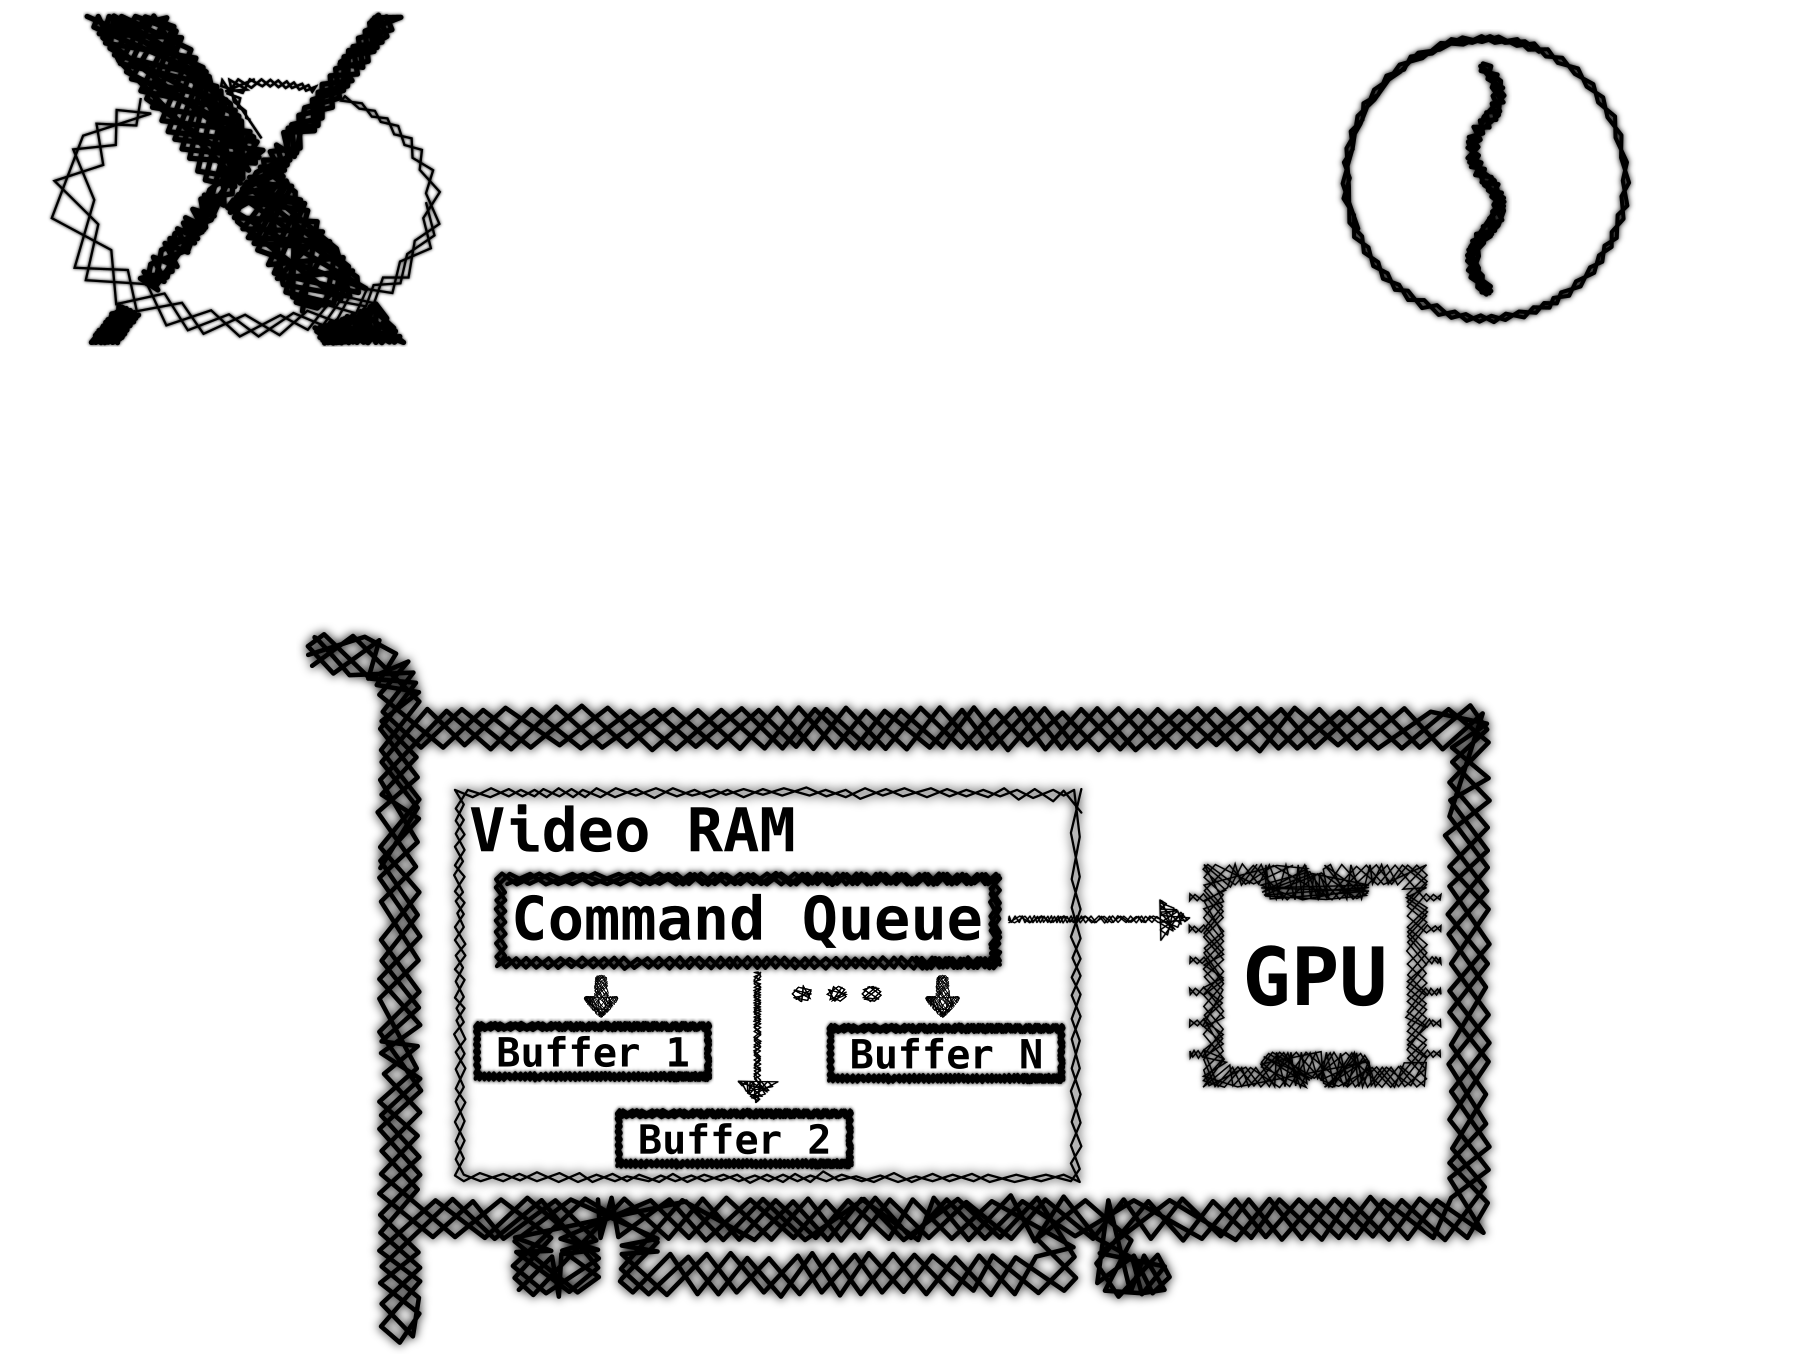
\includegraphics[width=\linewidth,
                     height=0.8\textheight,
                     keepaspectratio]{with_drm_1}
  \end{figure}
\end{frame}

\begin{frame}{100000 foot view}
  \begin{figure}
    \centering
    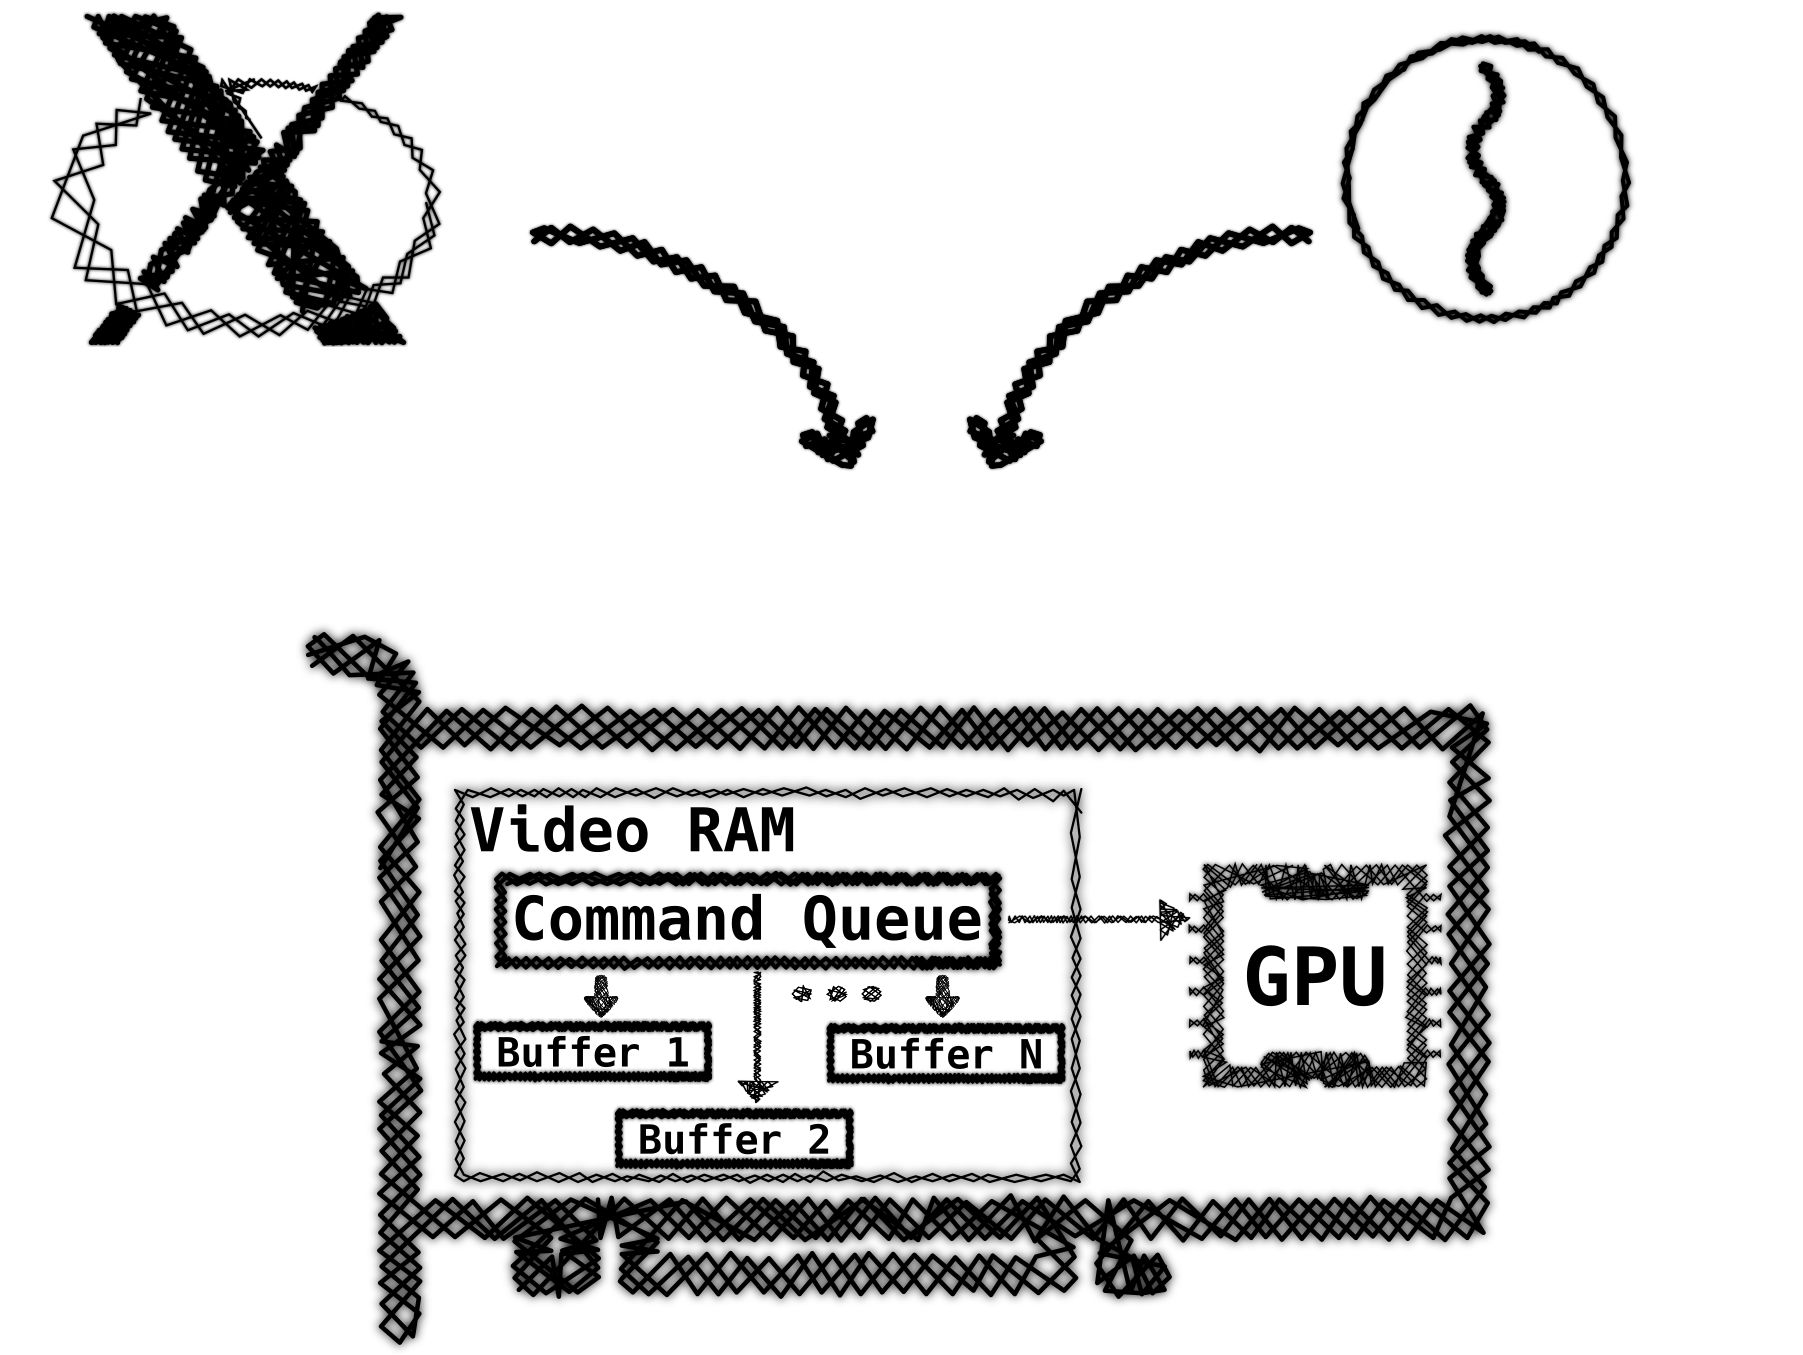
\includegraphics[width=\linewidth,
                     height=0.8\textheight,
                     keepaspectratio]{with_drm_2}
  \end{figure}
\end{frame}

\begin{frame}{100000 foot view}
  \begin{figure}
    \centering
    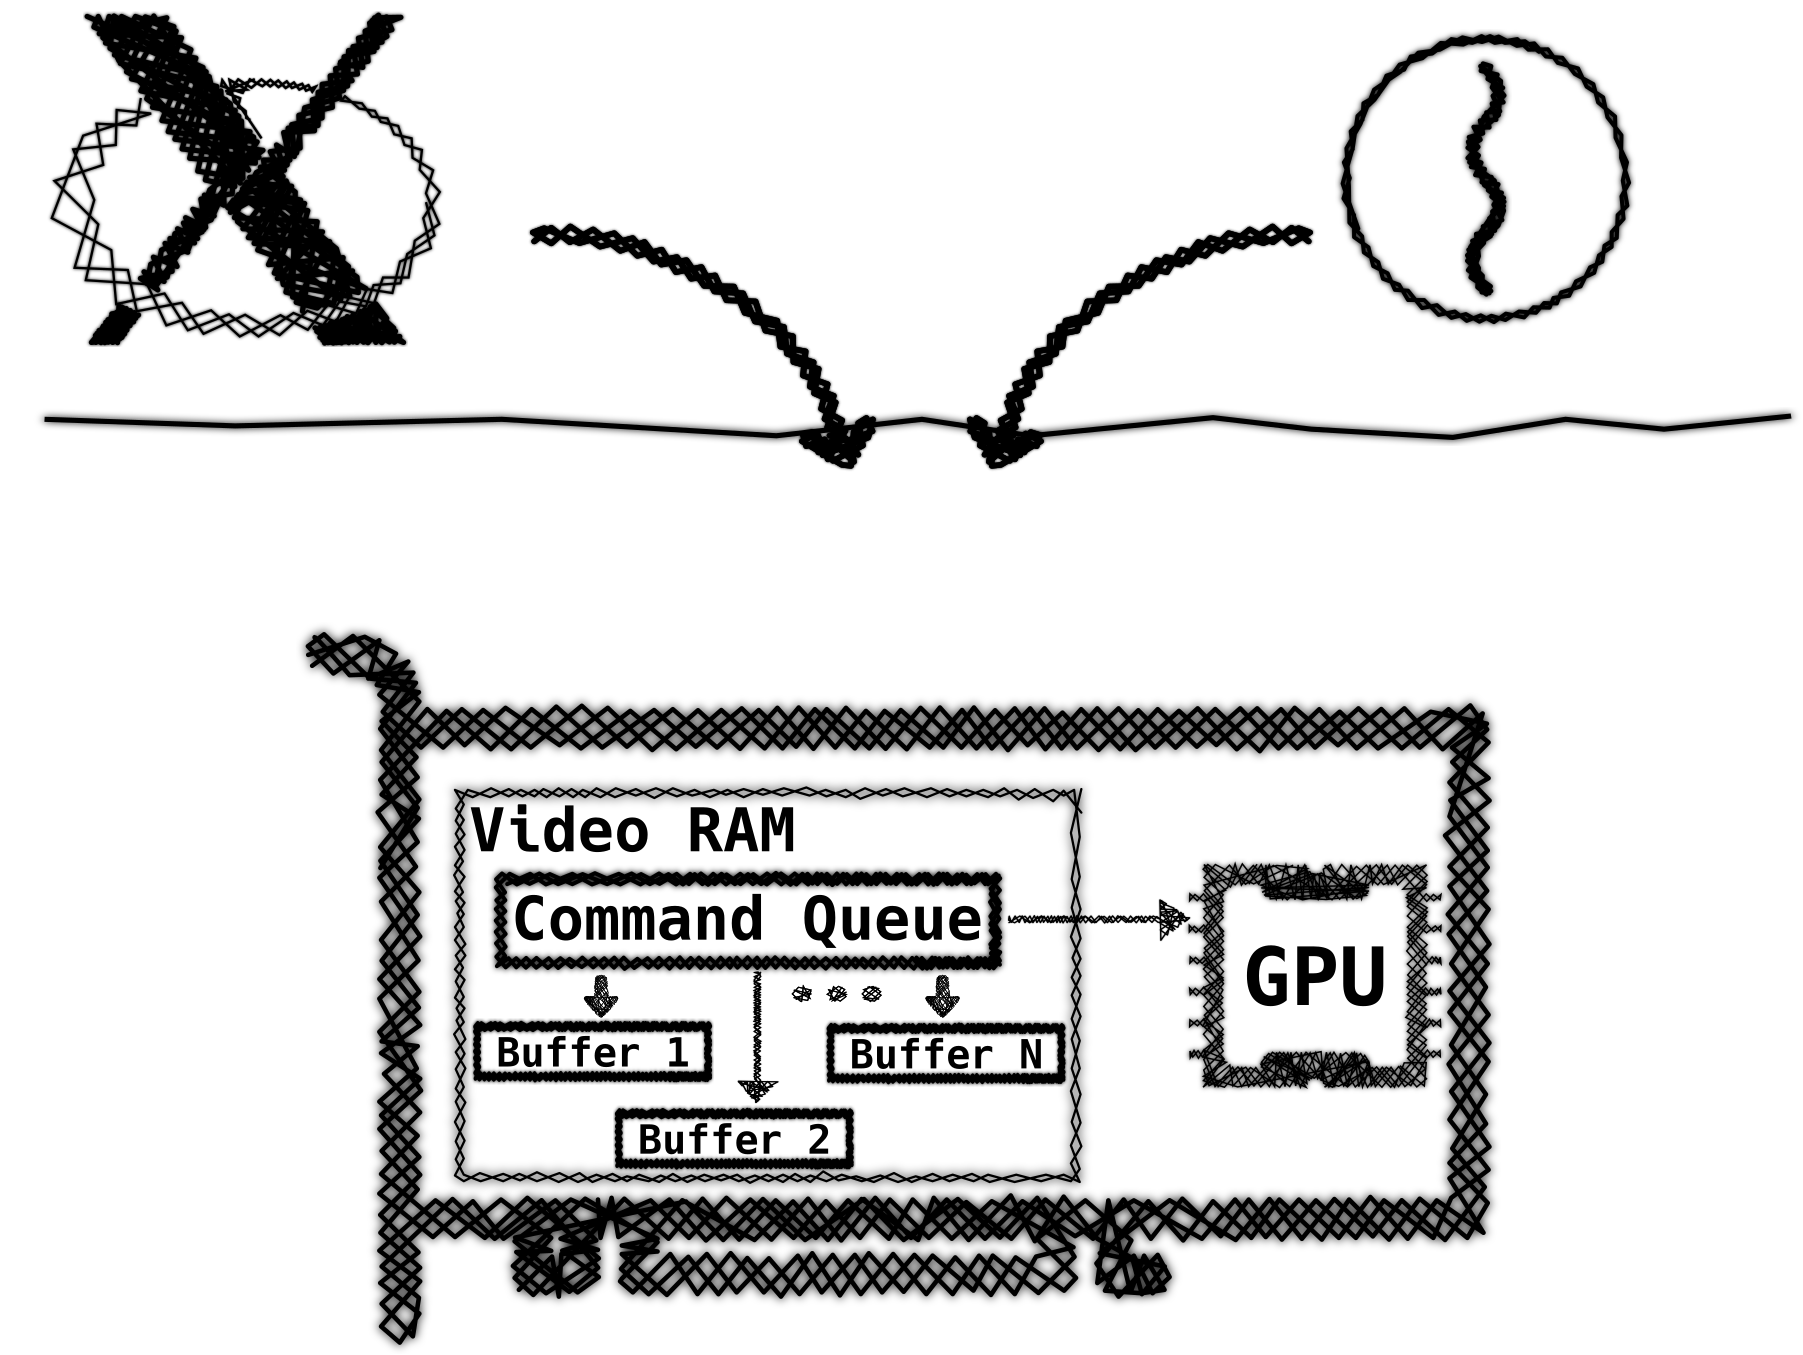
\includegraphics[width=\linewidth,
                     height=0.8\textheight,
                     keepaspectratio]{with_drm_3}
  \end{figure}
\end{frame}

\begin{frame}{100000 foot view}
  \begin{figure}
    \centering
    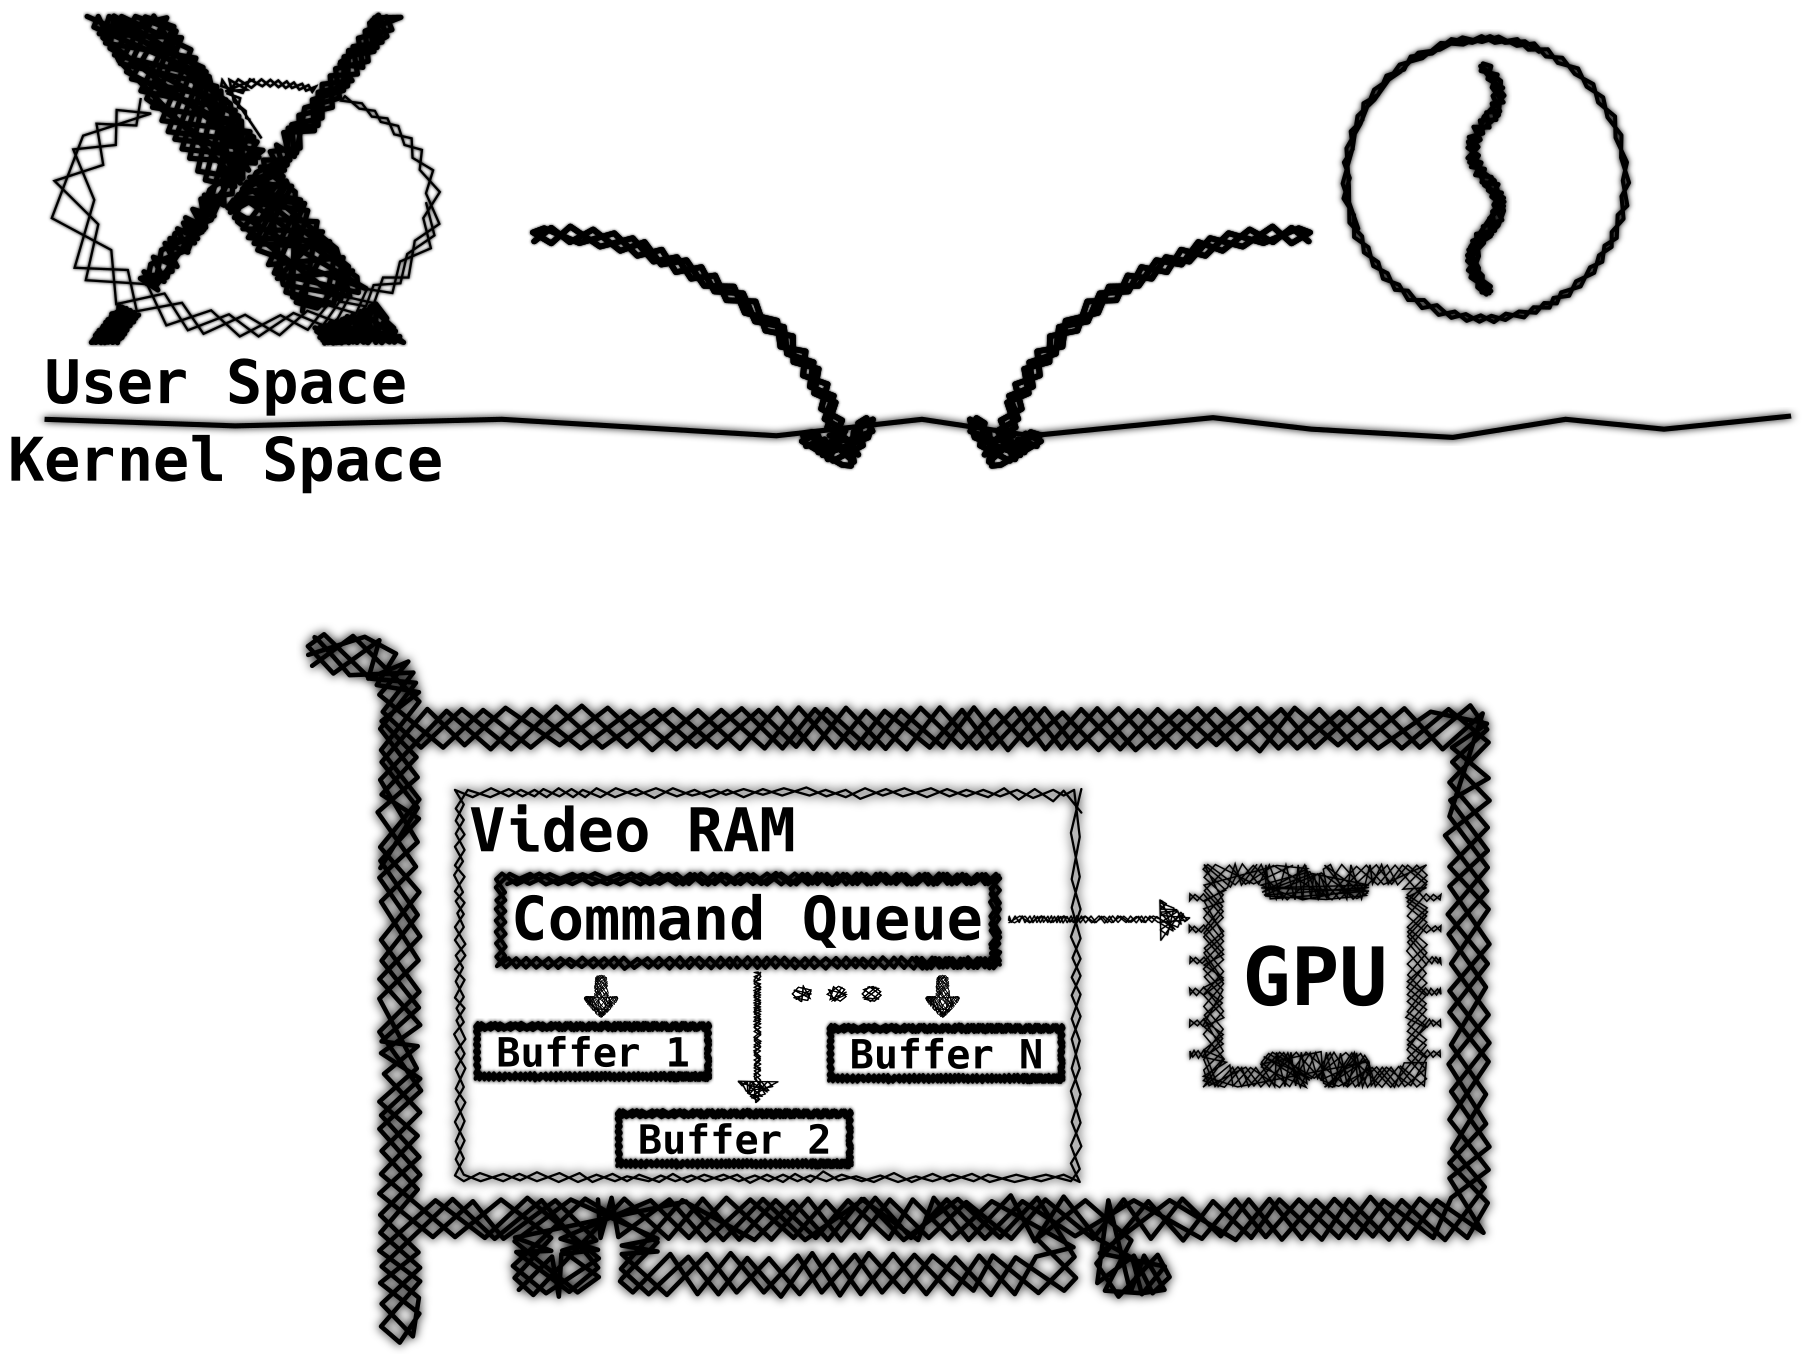
\includegraphics[width=\linewidth,
                     height=0.8\textheight,
                     keepaspectratio]{with_drm_4}
  \end{figure}
\end{frame}

\begin{frame}{100000 foot view}
  \begin{figure}
    \centering
    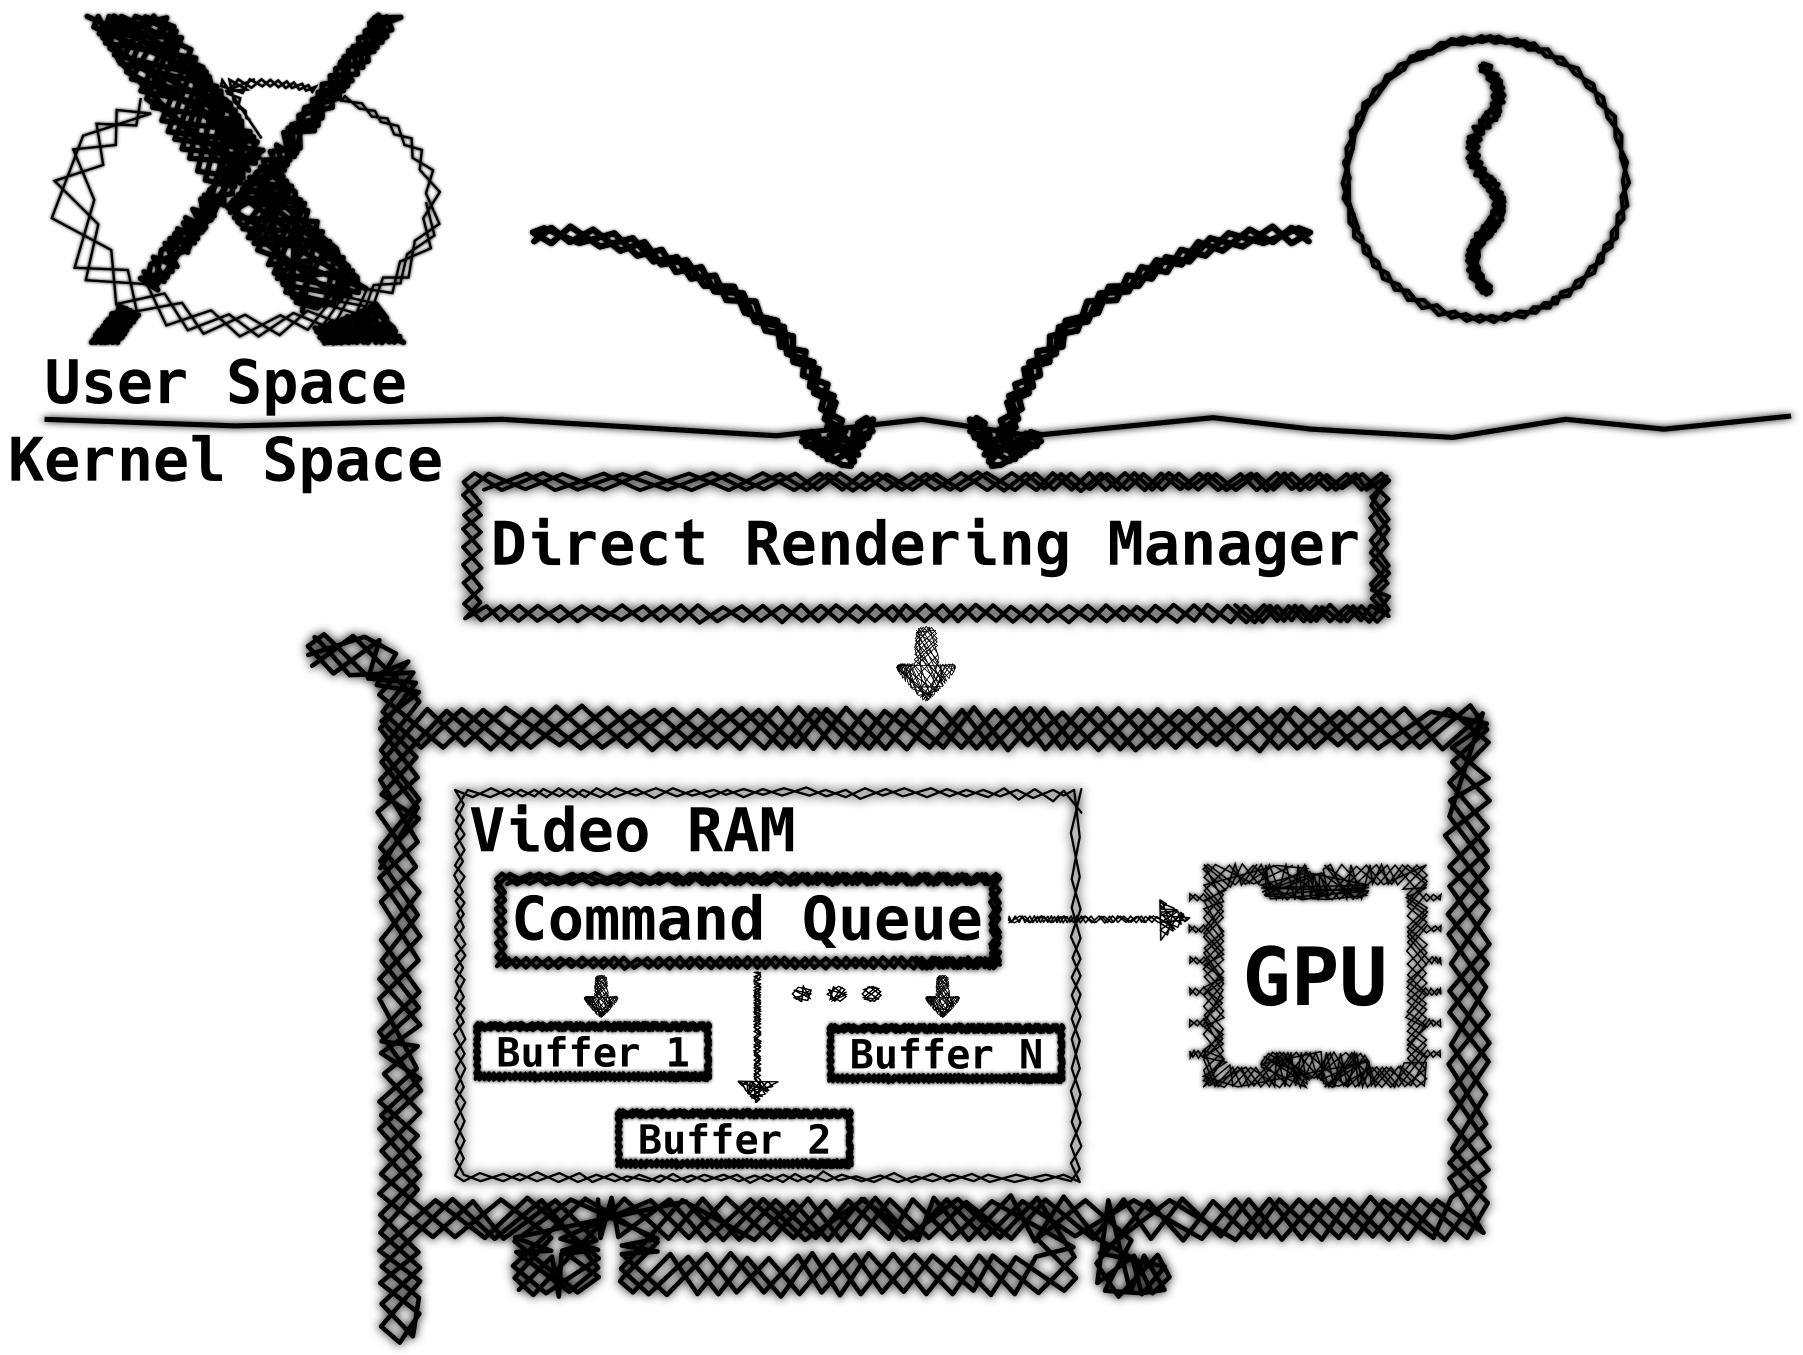
\includegraphics[width=\linewidth,
                     height=0.8\textheight,
                     keepaspectratio]{with_drm_5}
  \end{figure}
\end{frame}

\begin{frame}{100000 foot view}
  \metroset{block=fill}
  \begin{exampleblock}{Problems}
    \begin{itemize}
      \item Removes code duplication \pause
      \item KMS can use Kernel resources for providing better mechanisms \pause
      \item Clear separation between Kernel and User space \pause
      \item Manage resources
    \end{itemize}
  \end{exampleblock}
\end{frame}

%------------------------------------------------------------------------------
\section{10000 foot view}
\begin{frame}{10000 foot view}
  \begin{figure}
    \centering
    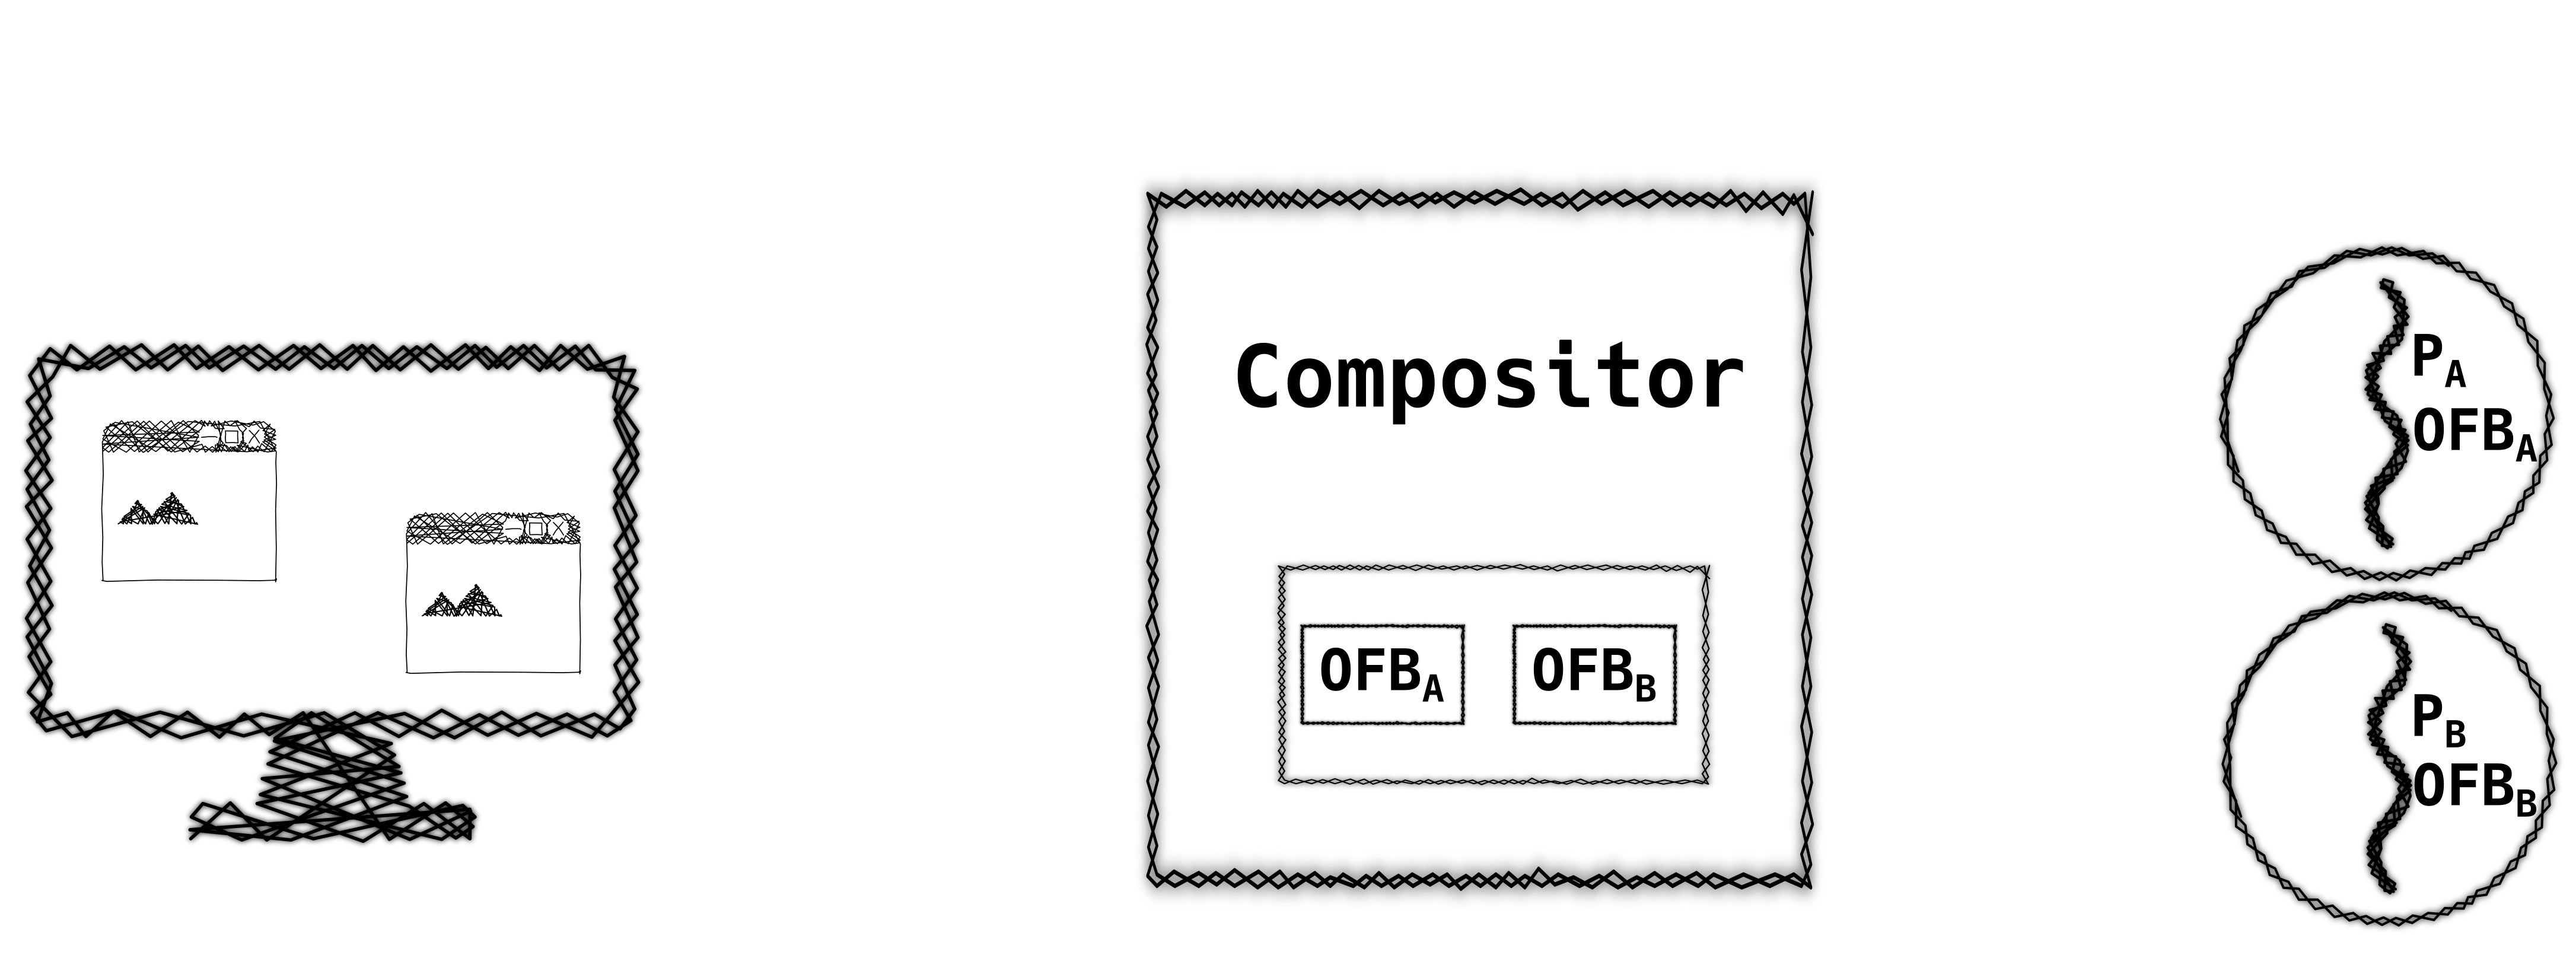
\includegraphics[width=\linewidth,
                     height=0.8\textheight,
                     keepaspectratio]{overview_graphics_drm_1-min}
  \end{figure}
\end{frame}

\begin{frame}{10000 foot view}
  \begin{figure}
    \centering
    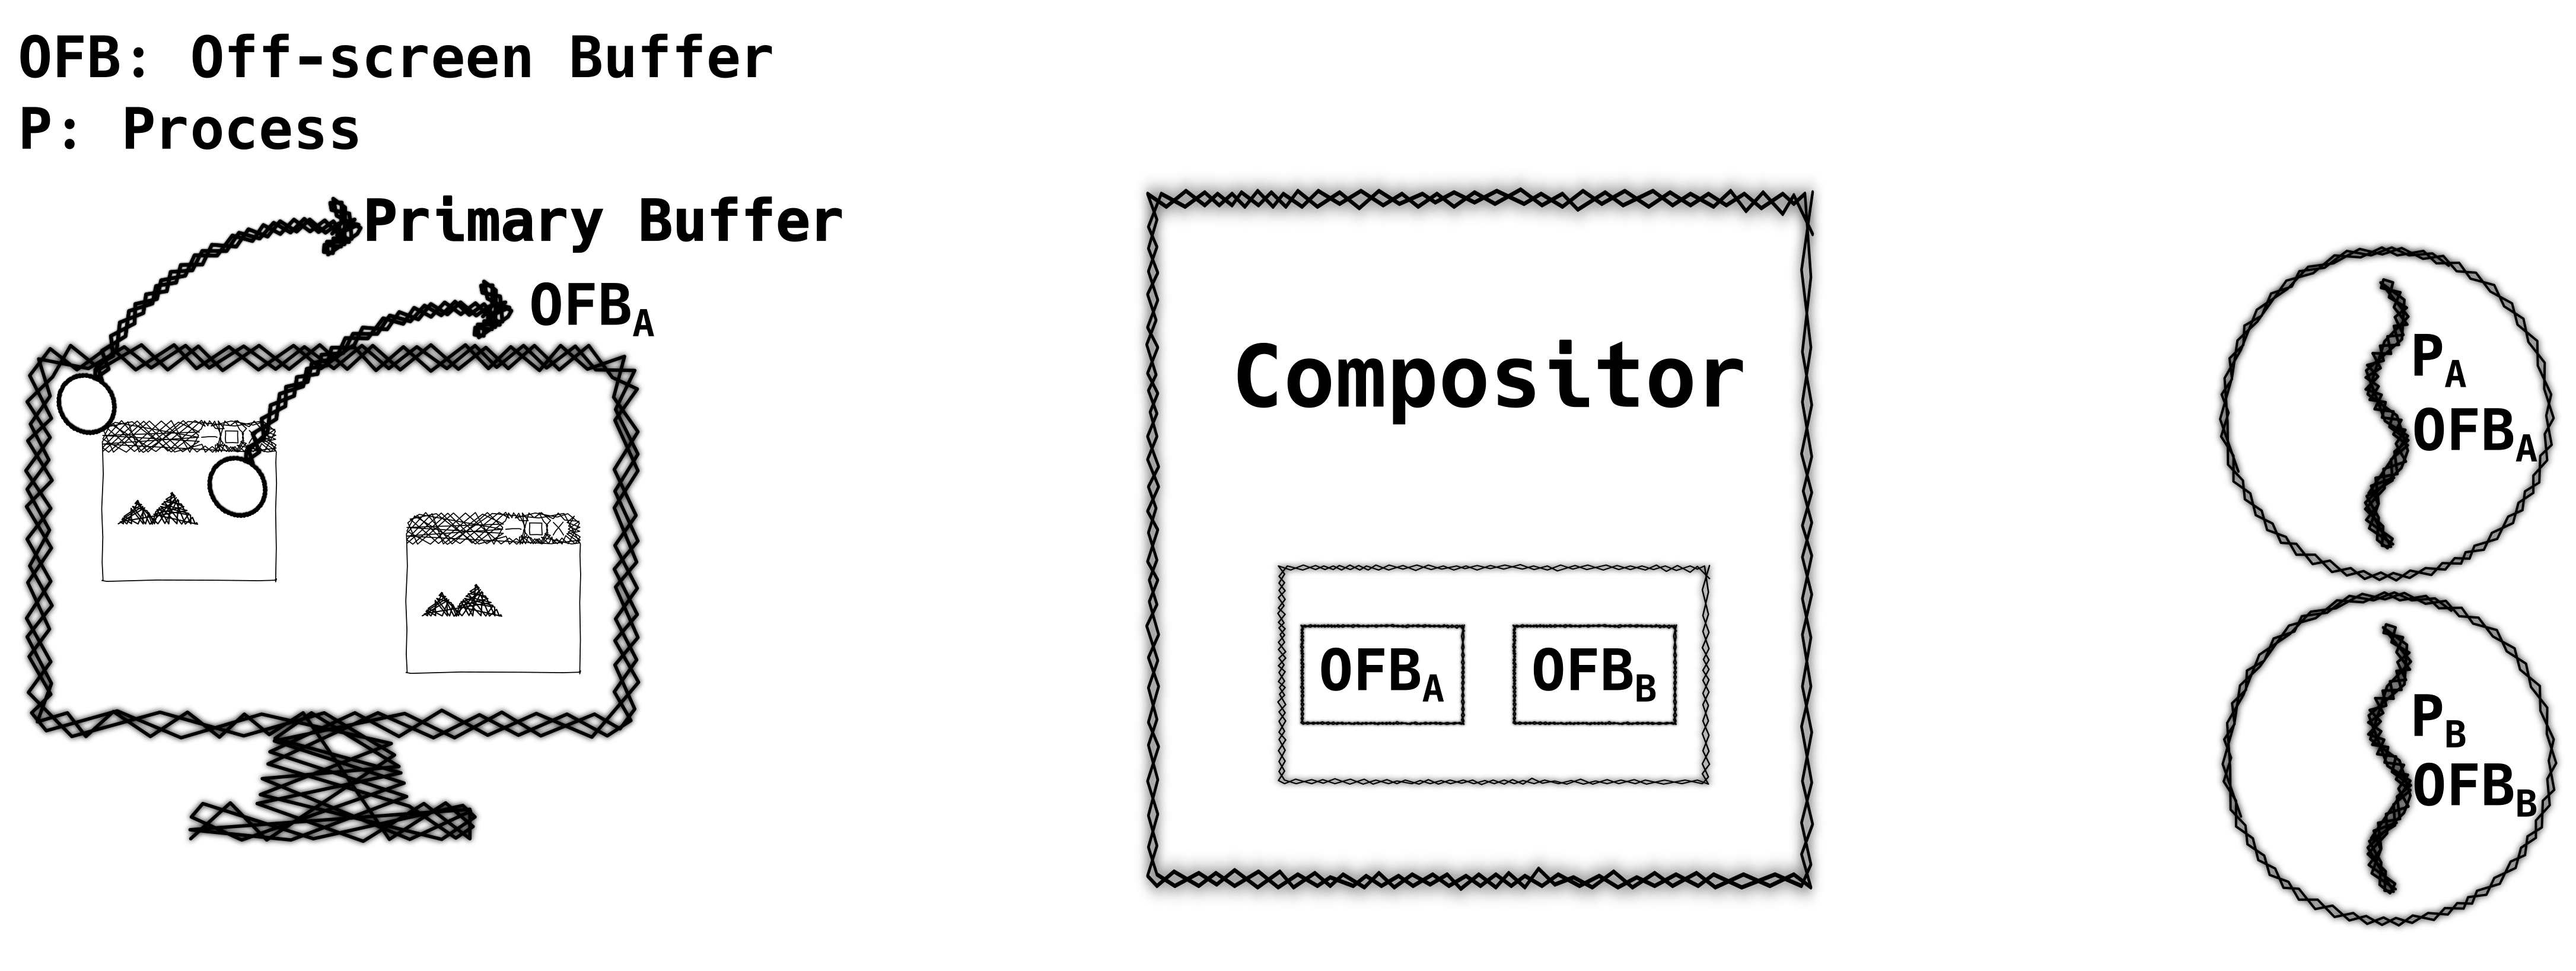
\includegraphics[width=\linewidth,
                     height=0.8\textheight,
                     keepaspectratio]{overview_graphics_drm_2-min}
  \end{figure}
\end{frame}

\begin{frame}{10000 foot view}
  \begin{figure}
    \centering
    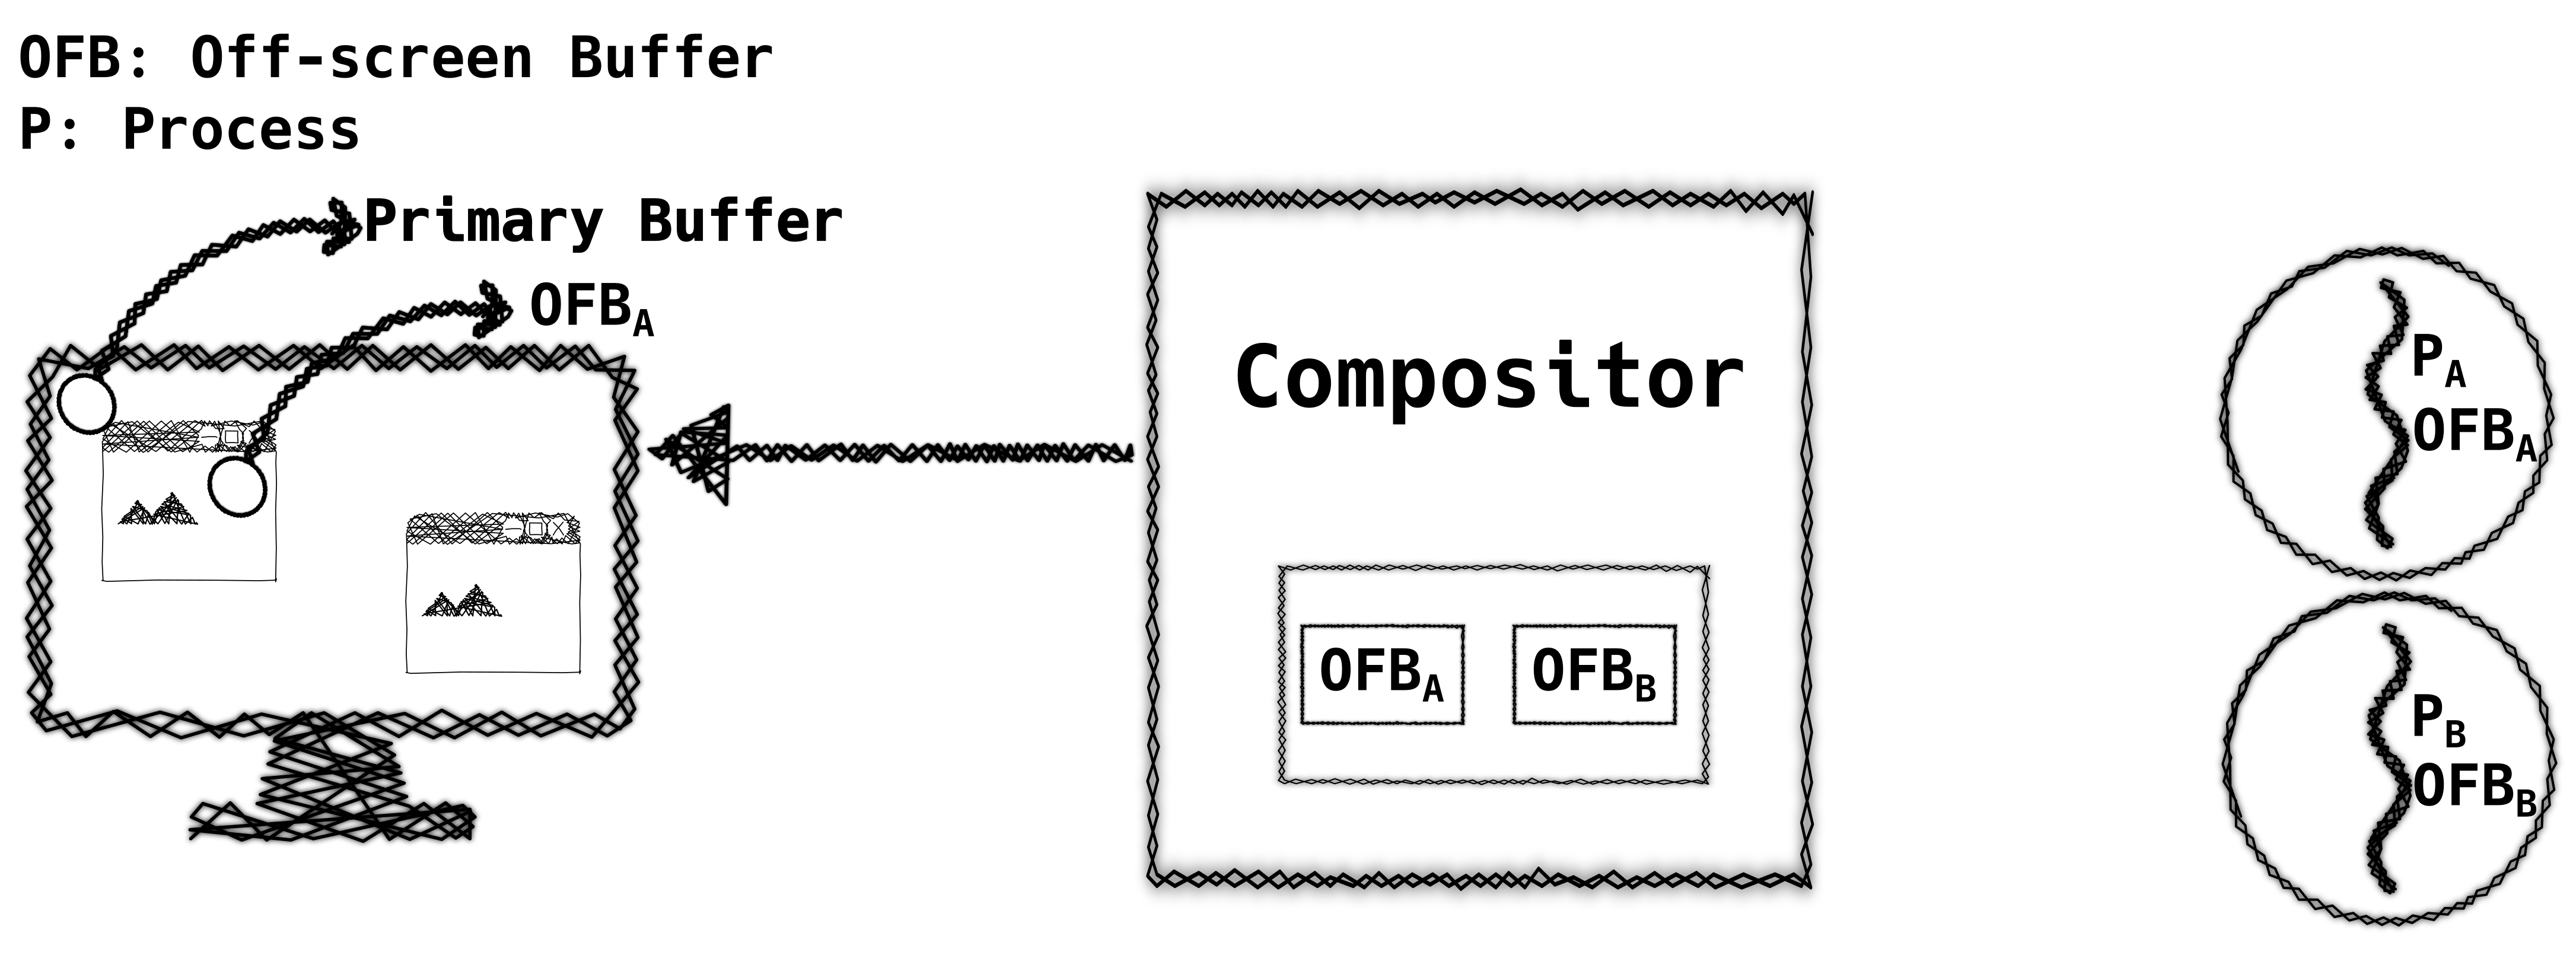
\includegraphics[width=\linewidth,
                     height=0.8\textheight,
                     keepaspectratio]{overview_graphics_drm_3-min}
  \end{figure}
\end{frame}

\begin{frame}{10000 foot view}
  \begin{figure}
    \centering
    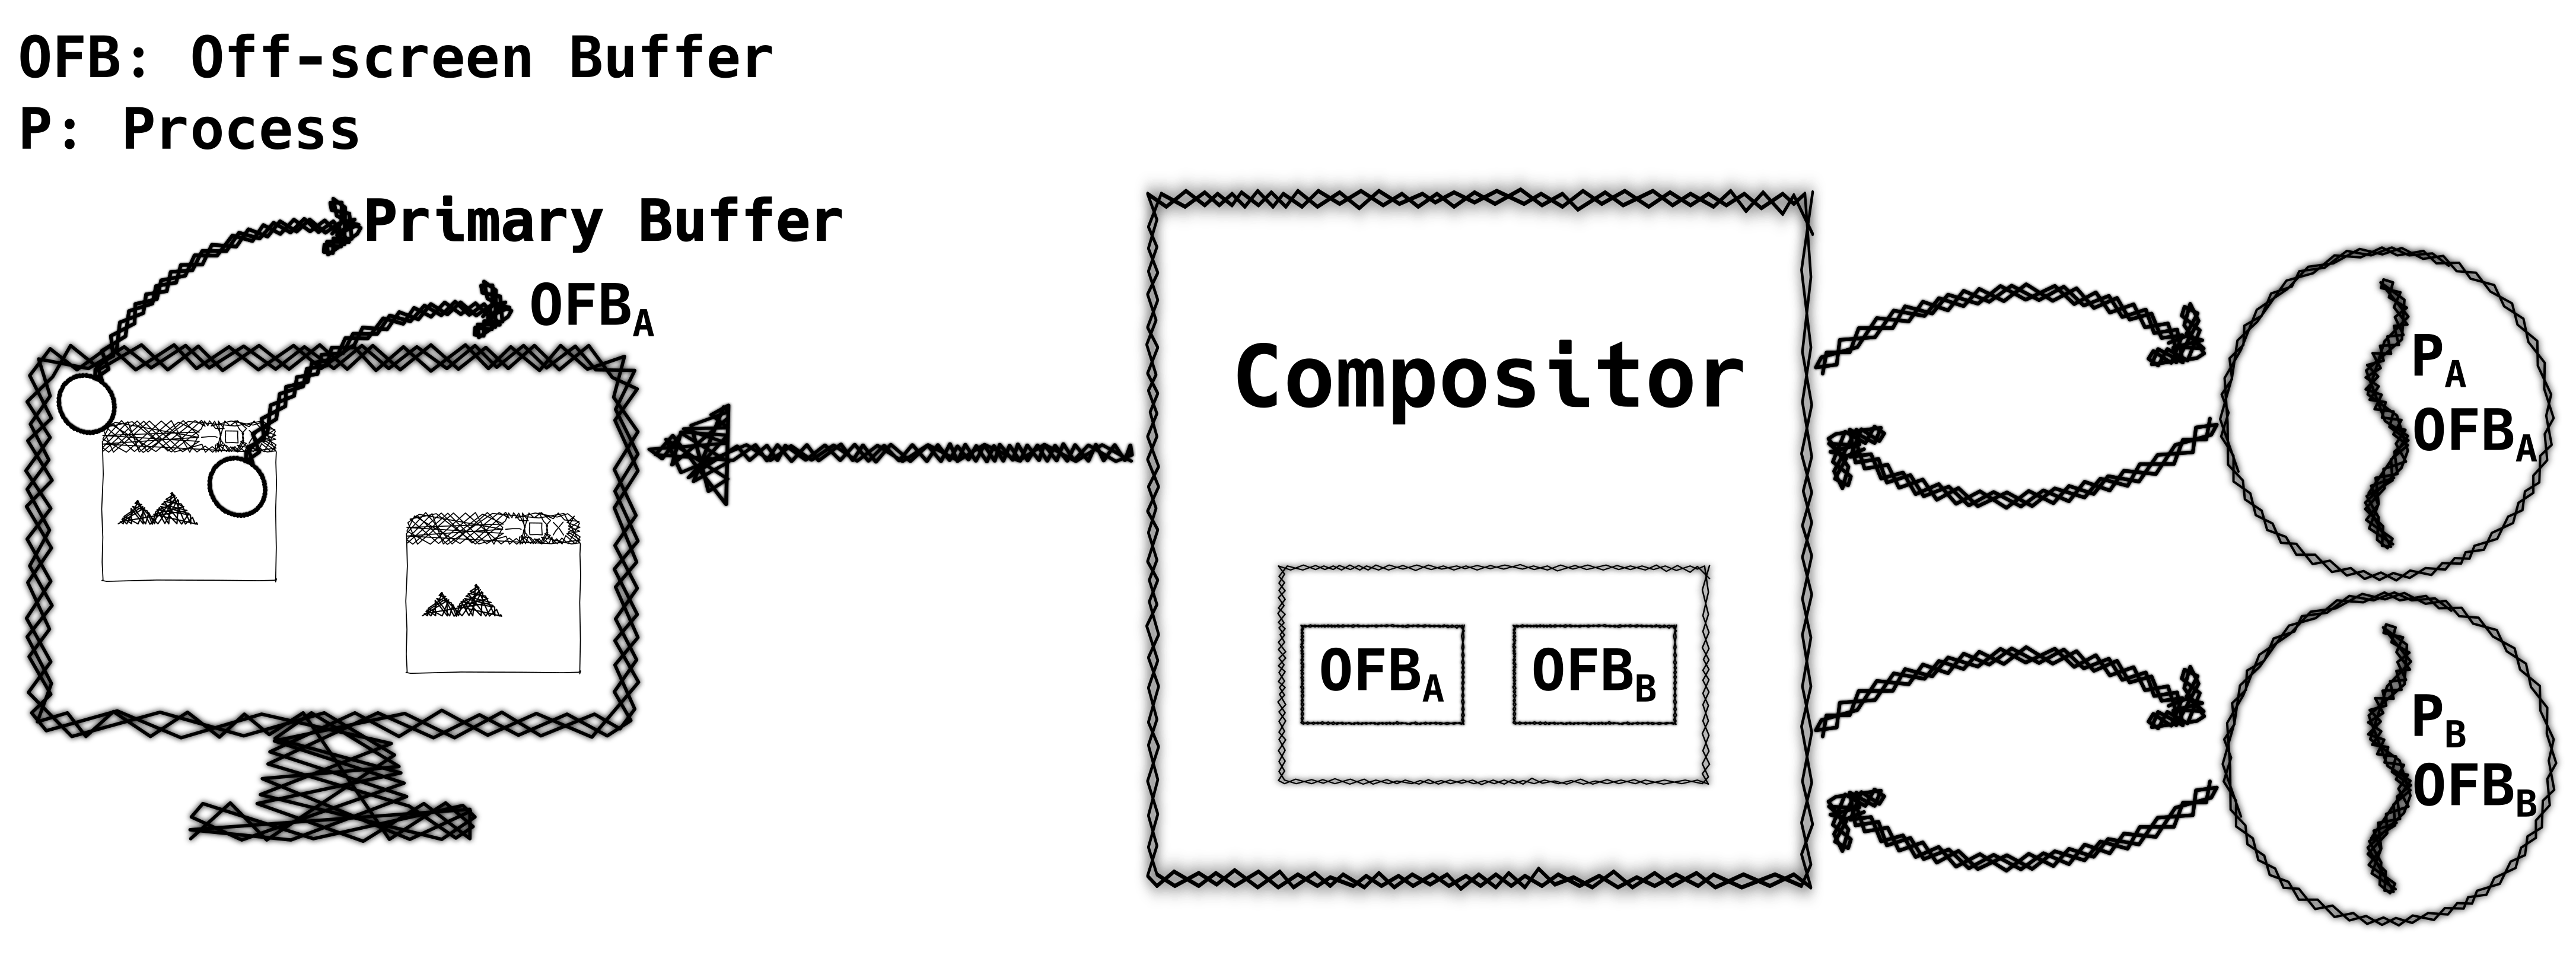
\includegraphics[width=\linewidth,
                     height=0.8\textheight,
                     keepaspectratio]{overview_graphics_drm_4-min}
  \end{figure}
\end{frame}

%------------------------------------------------------------------------------
\section{1000 foot view}
\begin{frame}{1000 foot view}
  \begin{figure}
    \centering
    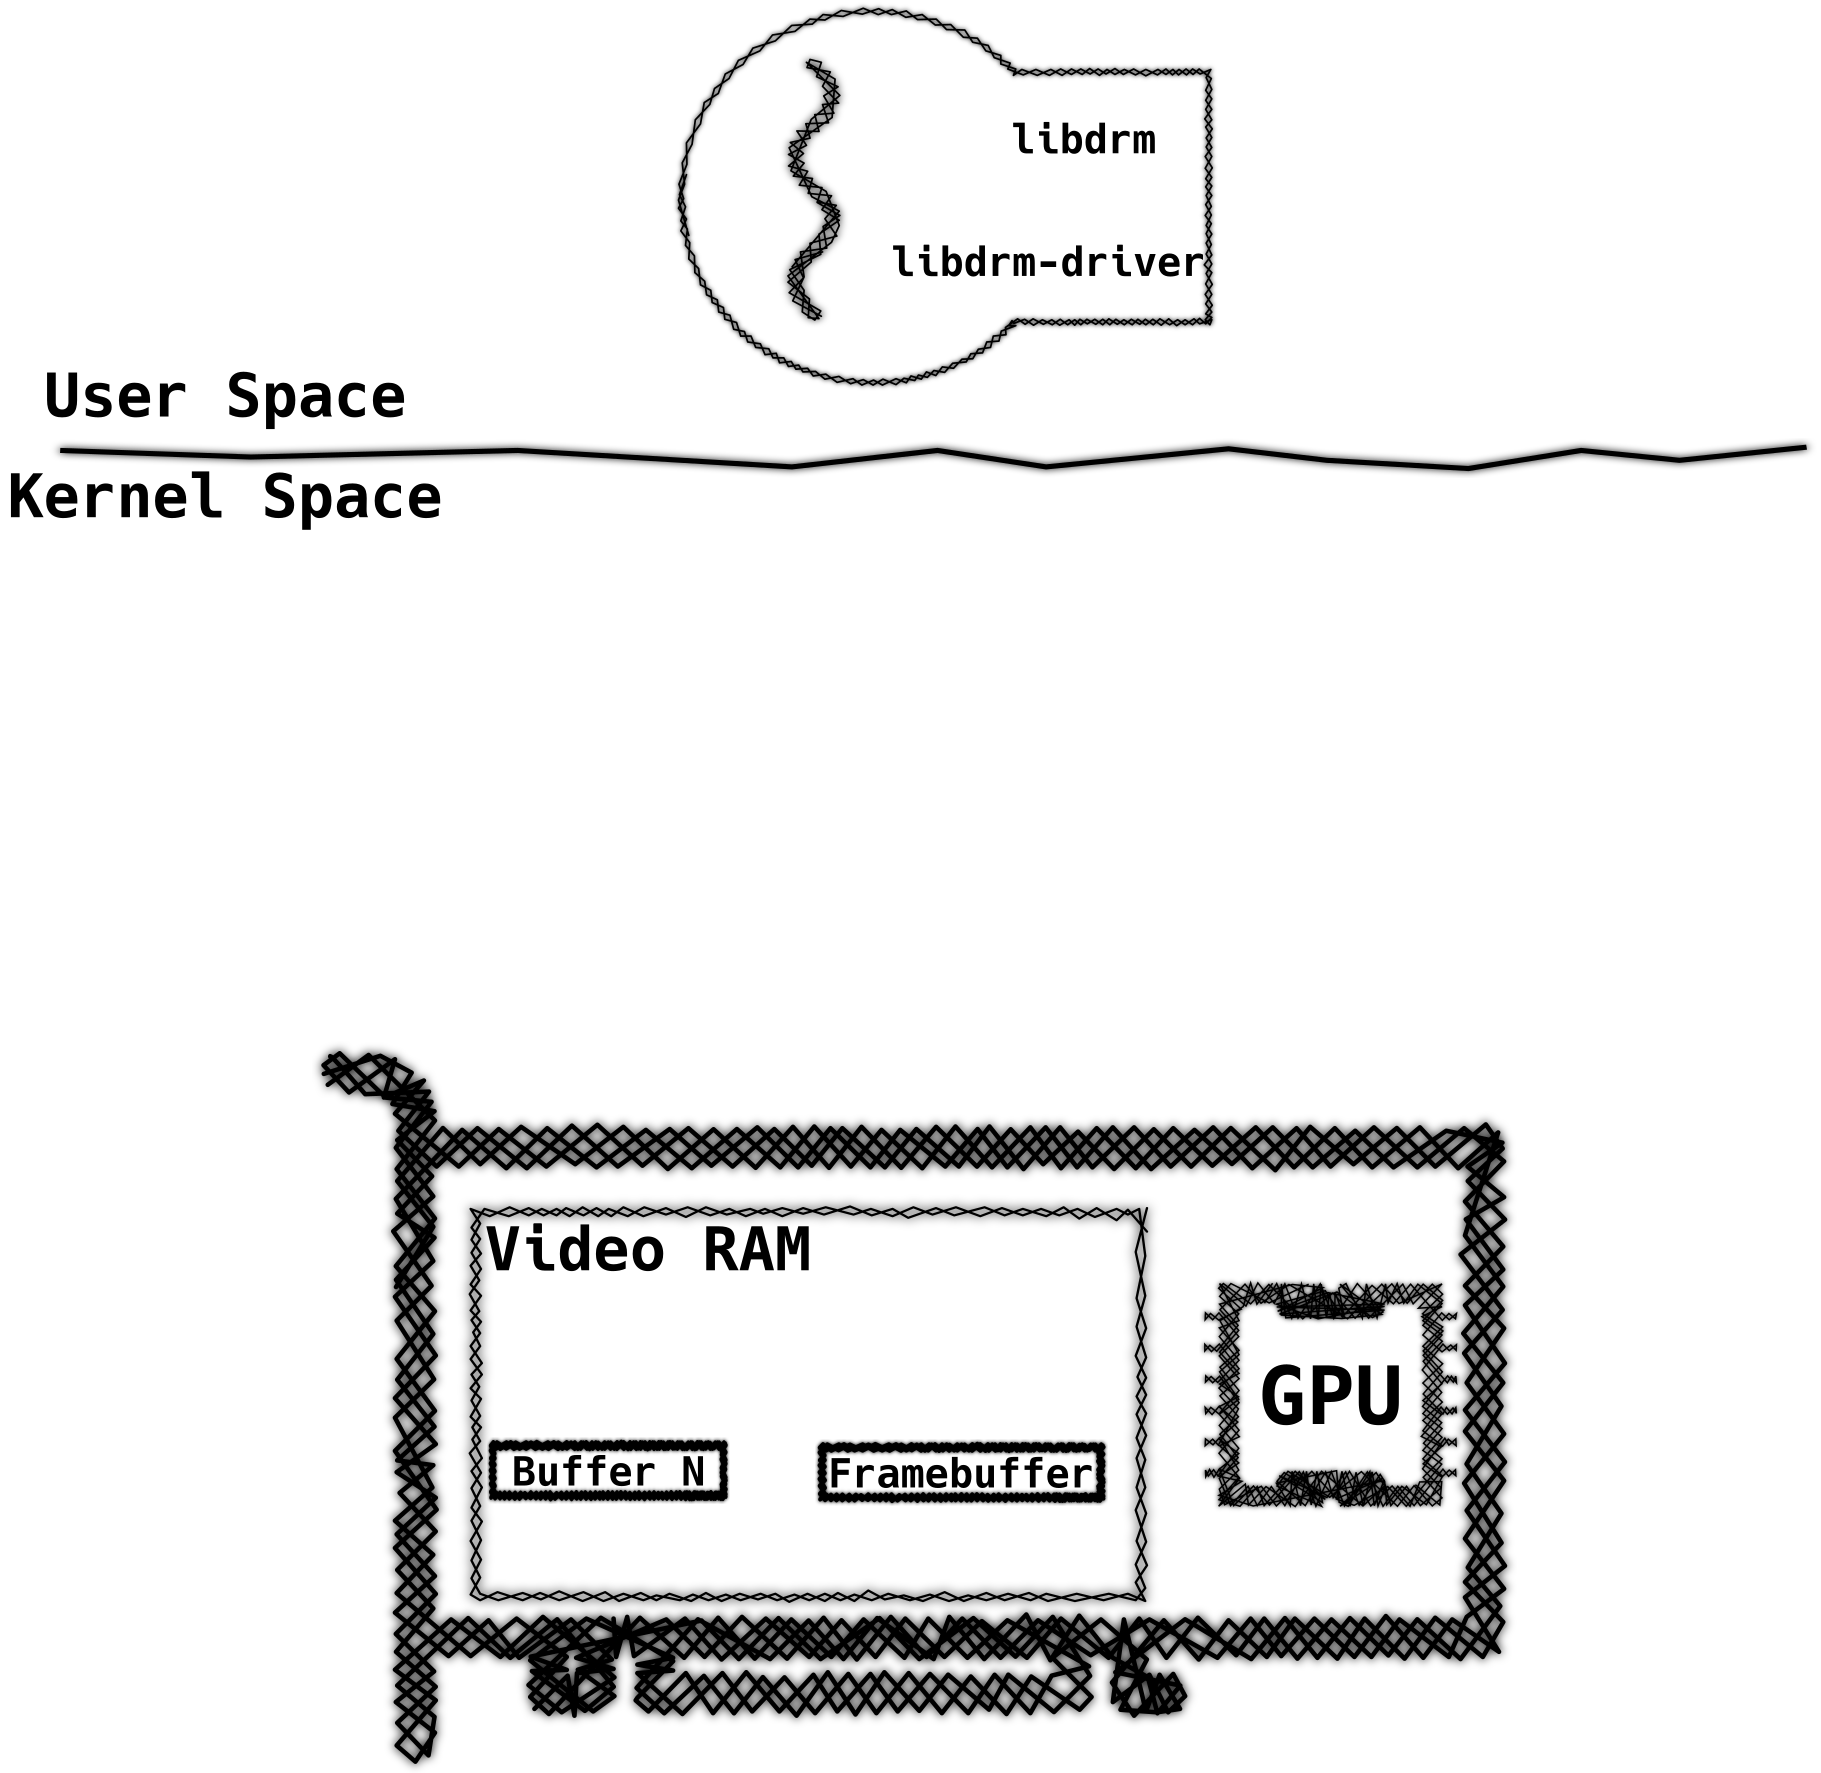
\includegraphics[width=\linewidth,
                     height=0.8\textheight,
                     keepaspectratio]{drm_api_1}
  \end{figure}
\end{frame}


\begin{frame}{1000 foot view}
  \begin{figure}
    \centering
    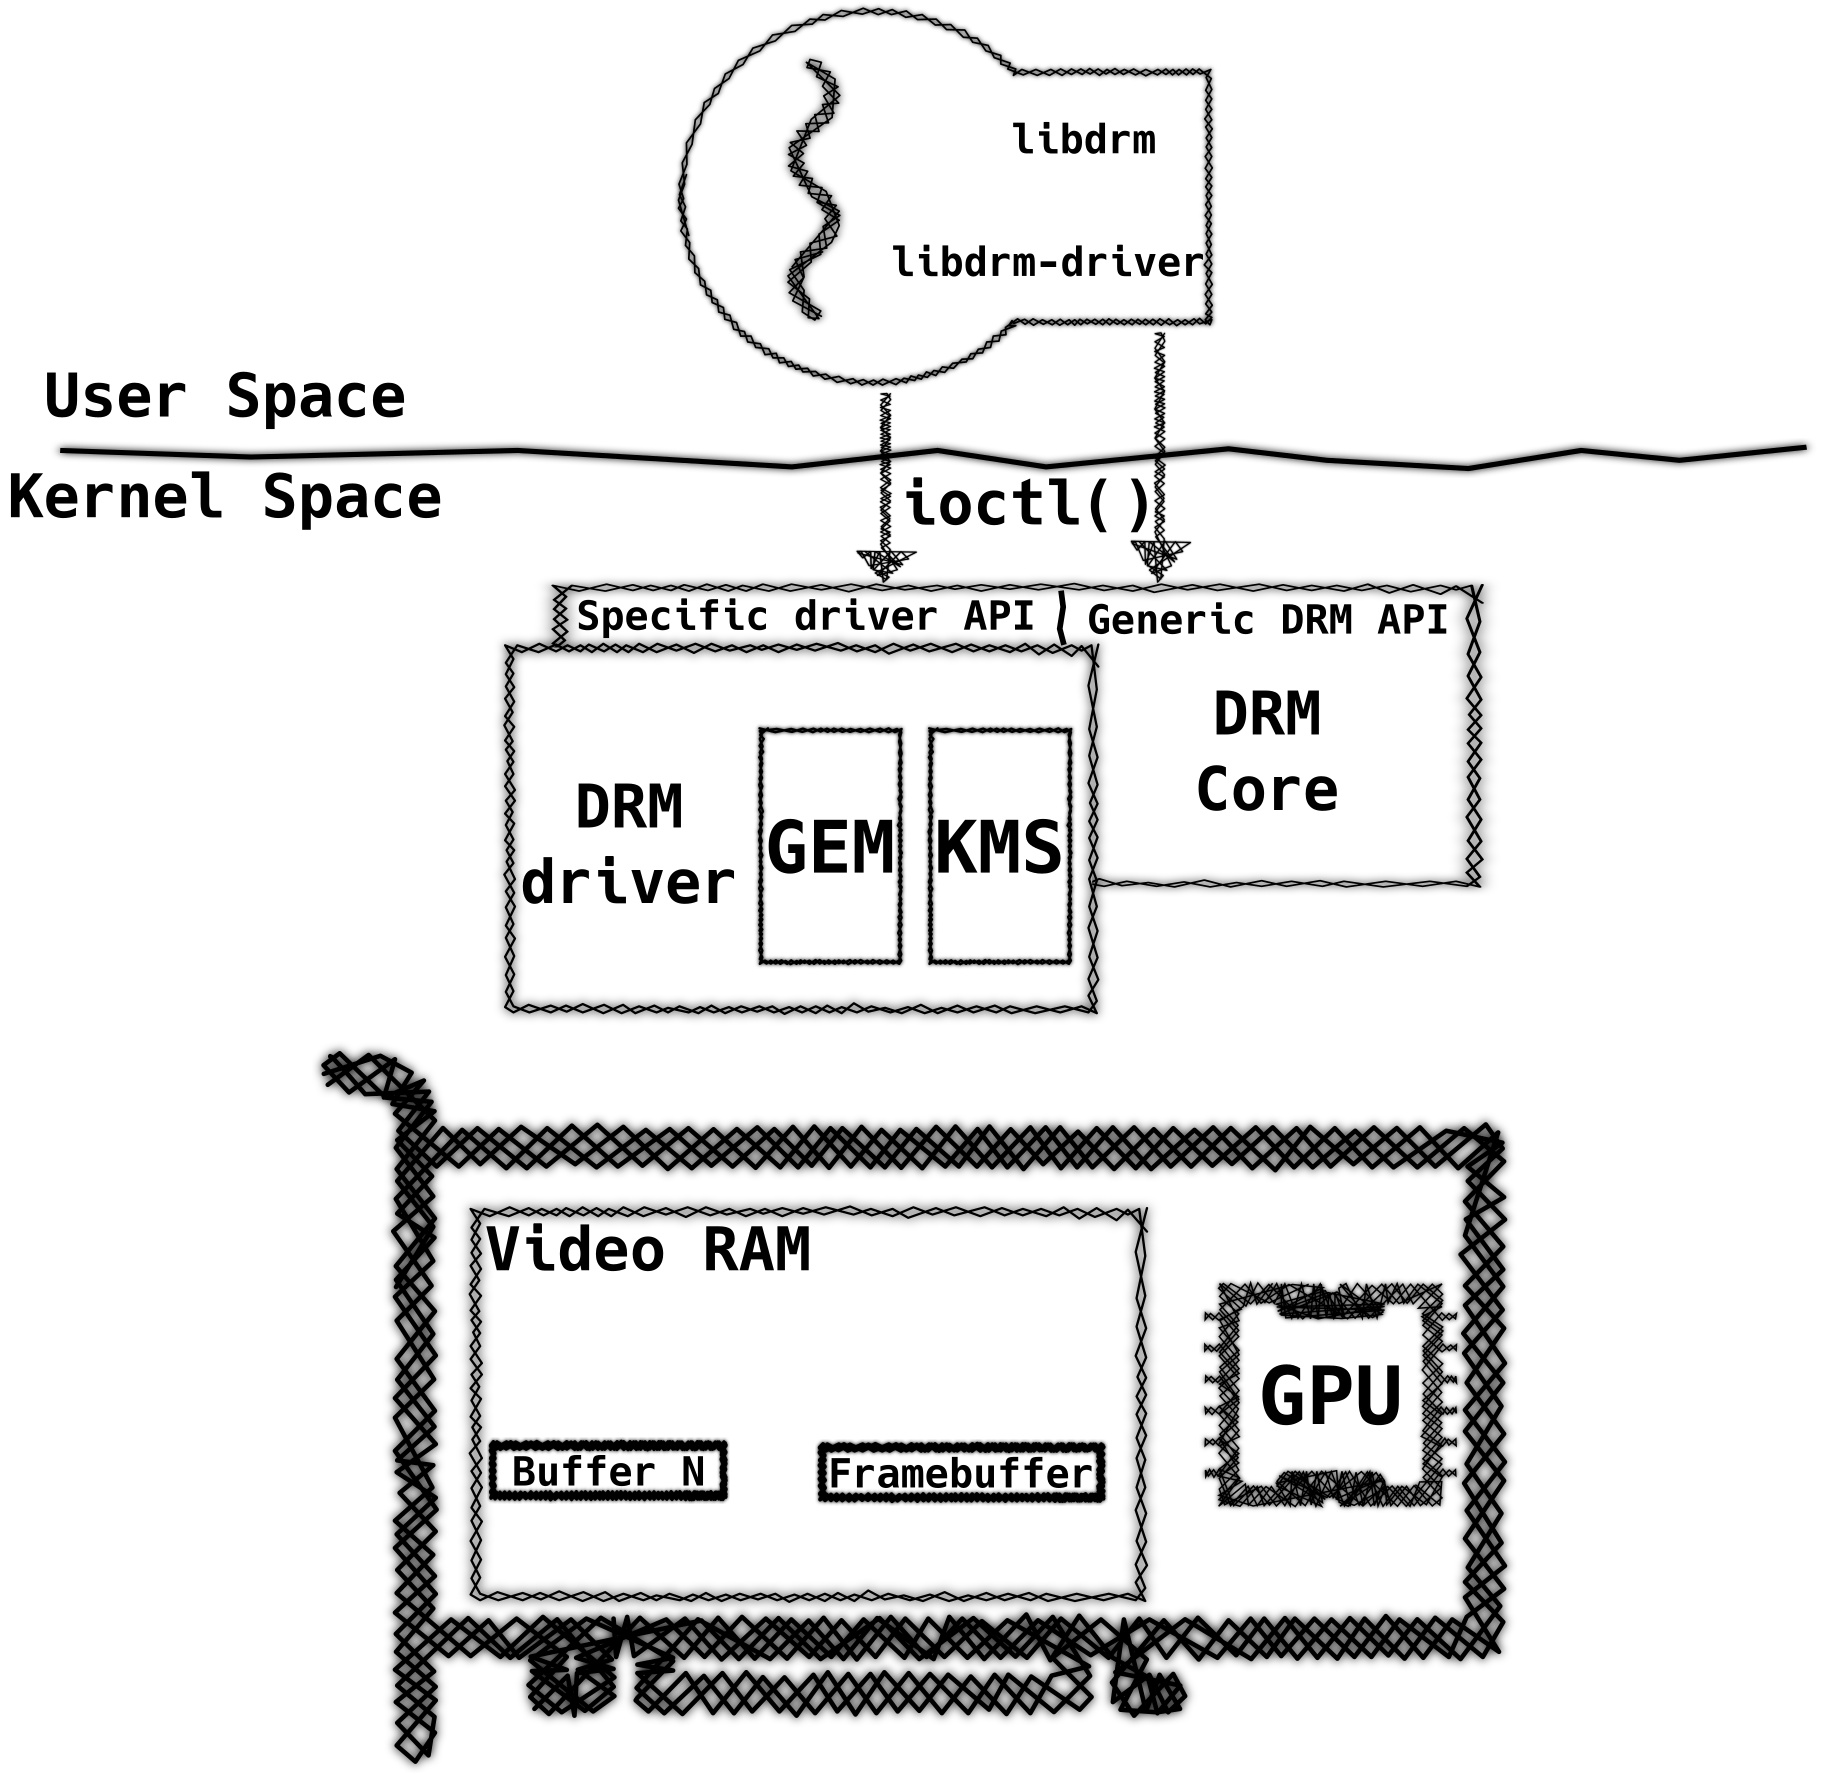
\includegraphics[width=\linewidth,
                     height=0.8\textheight,
                     keepaspectratio]{drm_api_2}
  \end{figure}
\end{frame}

\begin{frame}{1000 foot view}
  \begin{figure}
    \centering
    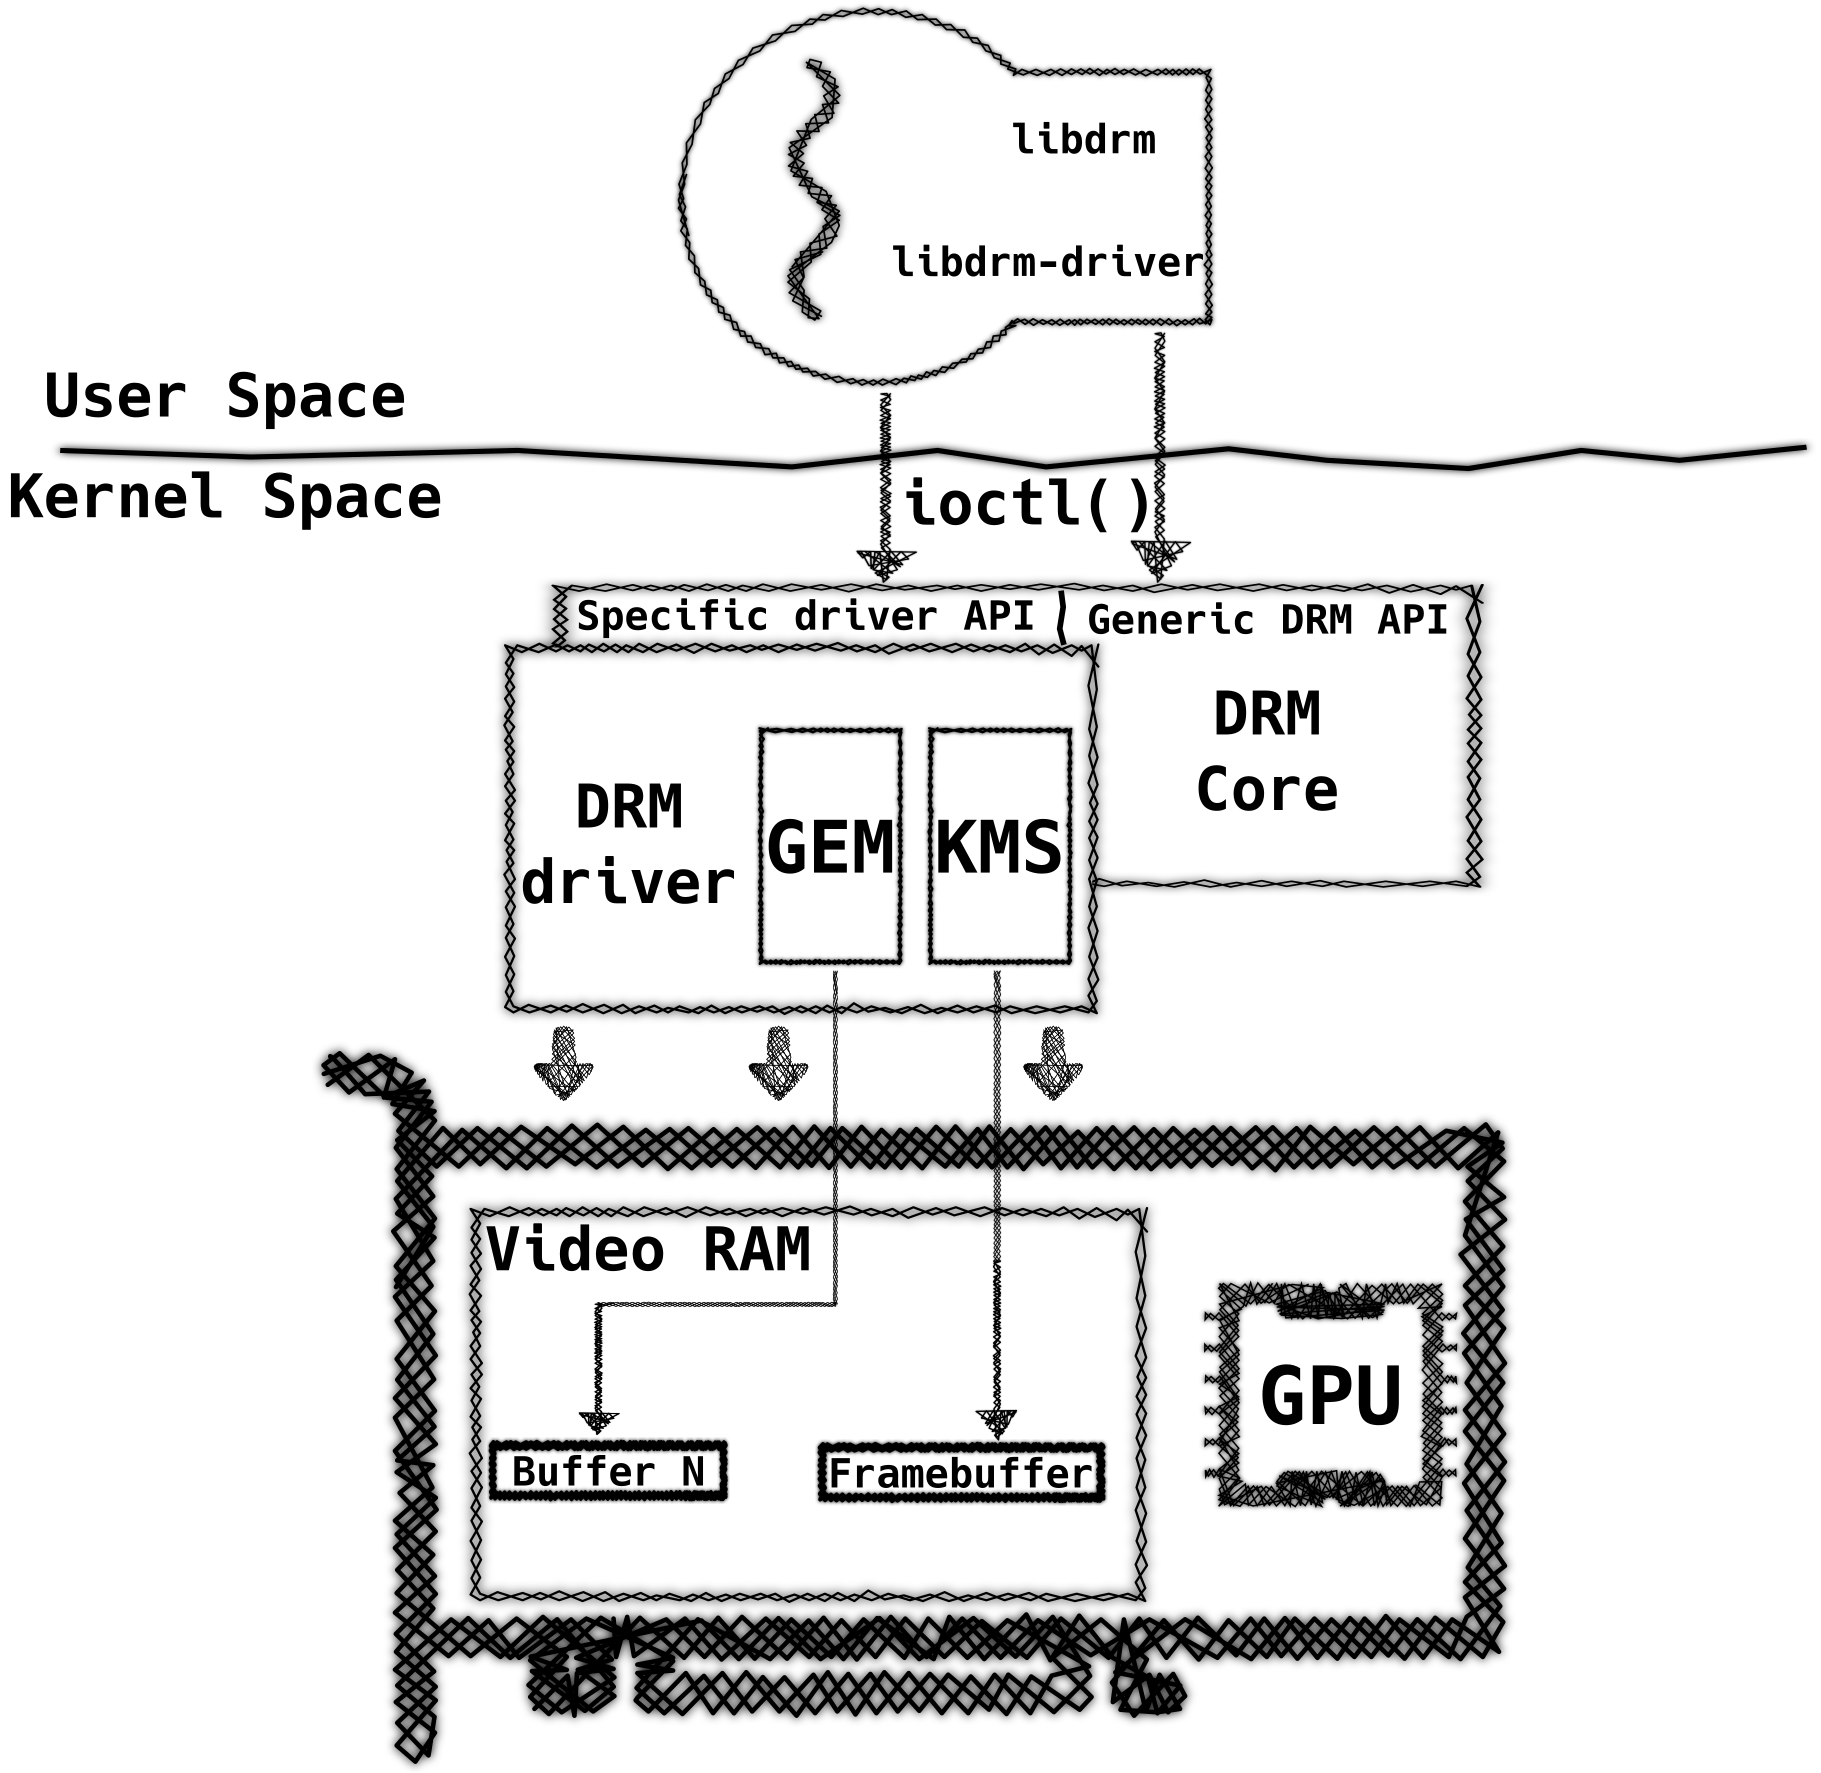
\includegraphics[width=\linewidth,
                     height=0.8\textheight,
                     keepaspectratio]{drm_api_3}
  \end{figure}
\end{frame}

%------------------------------------------------------------------------------
\section{100 foot view}
\begin{frame}{100 foot view}
  \begin{figure}
    \centering
    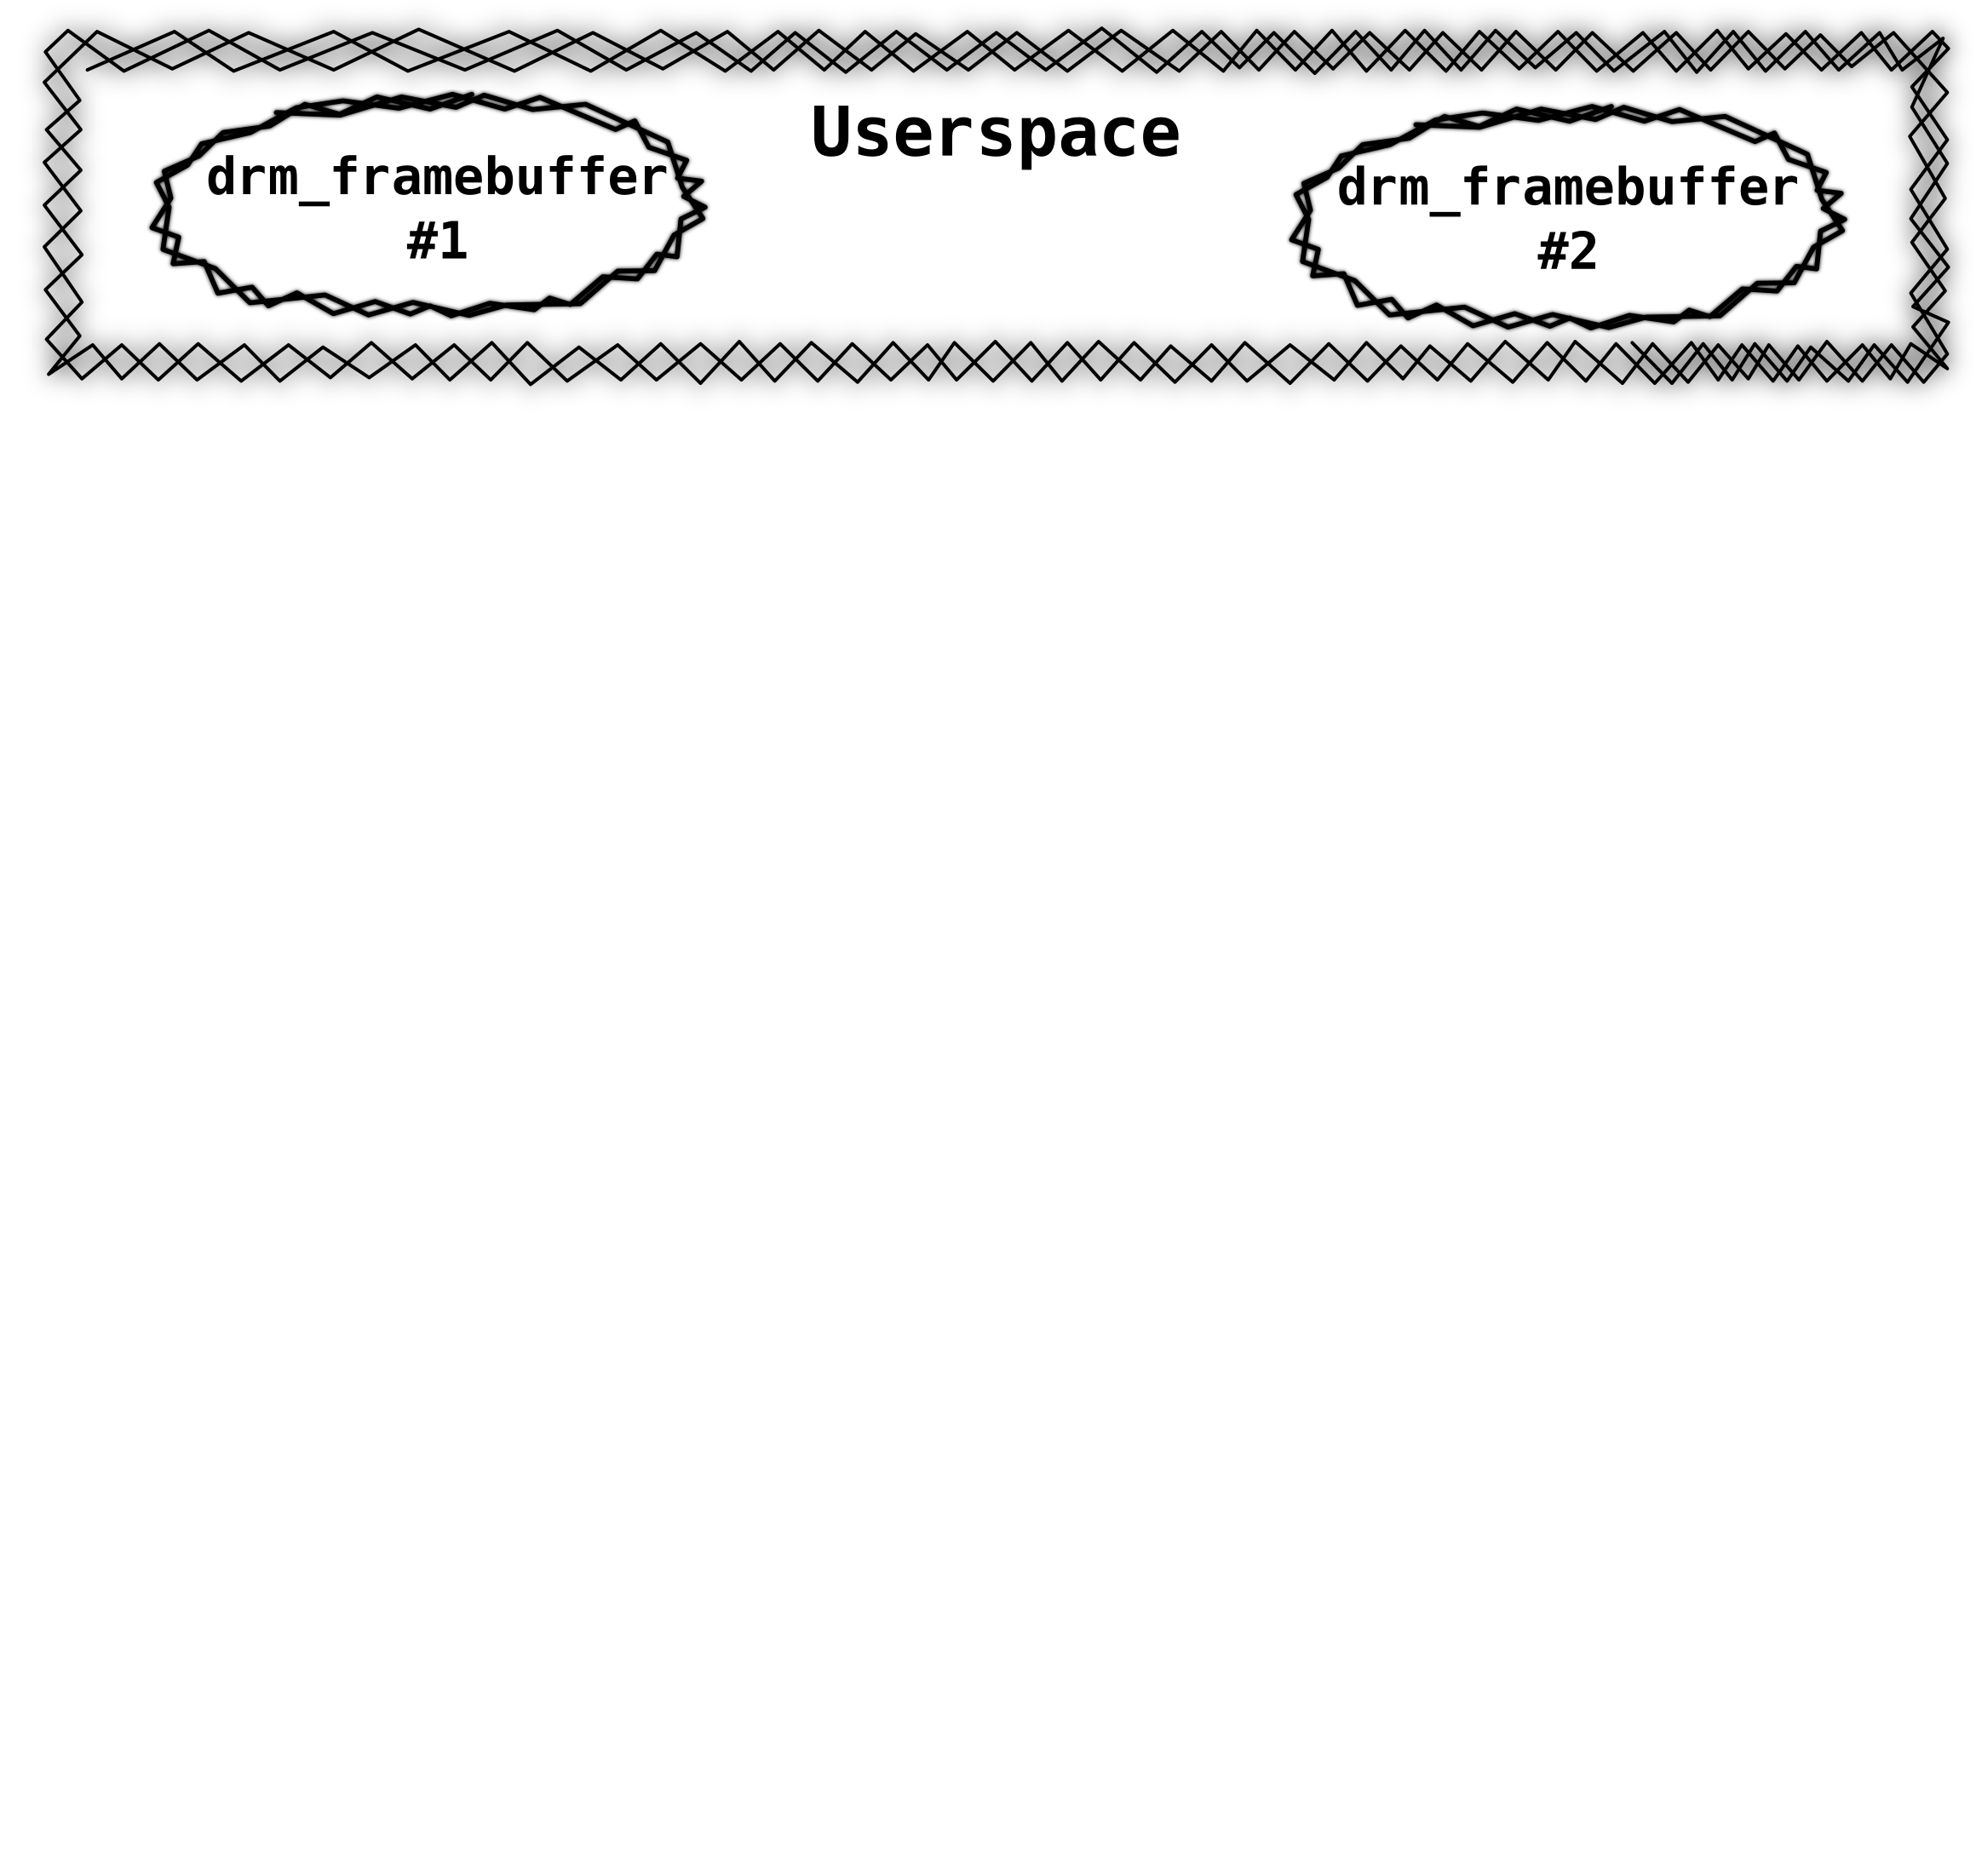
\includegraphics[width=\linewidth,
                     height=0.8\textheight,
                     keepaspectratio]{drm_internals_1}
  \end{figure}
\end{frame}

\begin{frame}{100 foot view}
  \begin{figure}
    \centering
    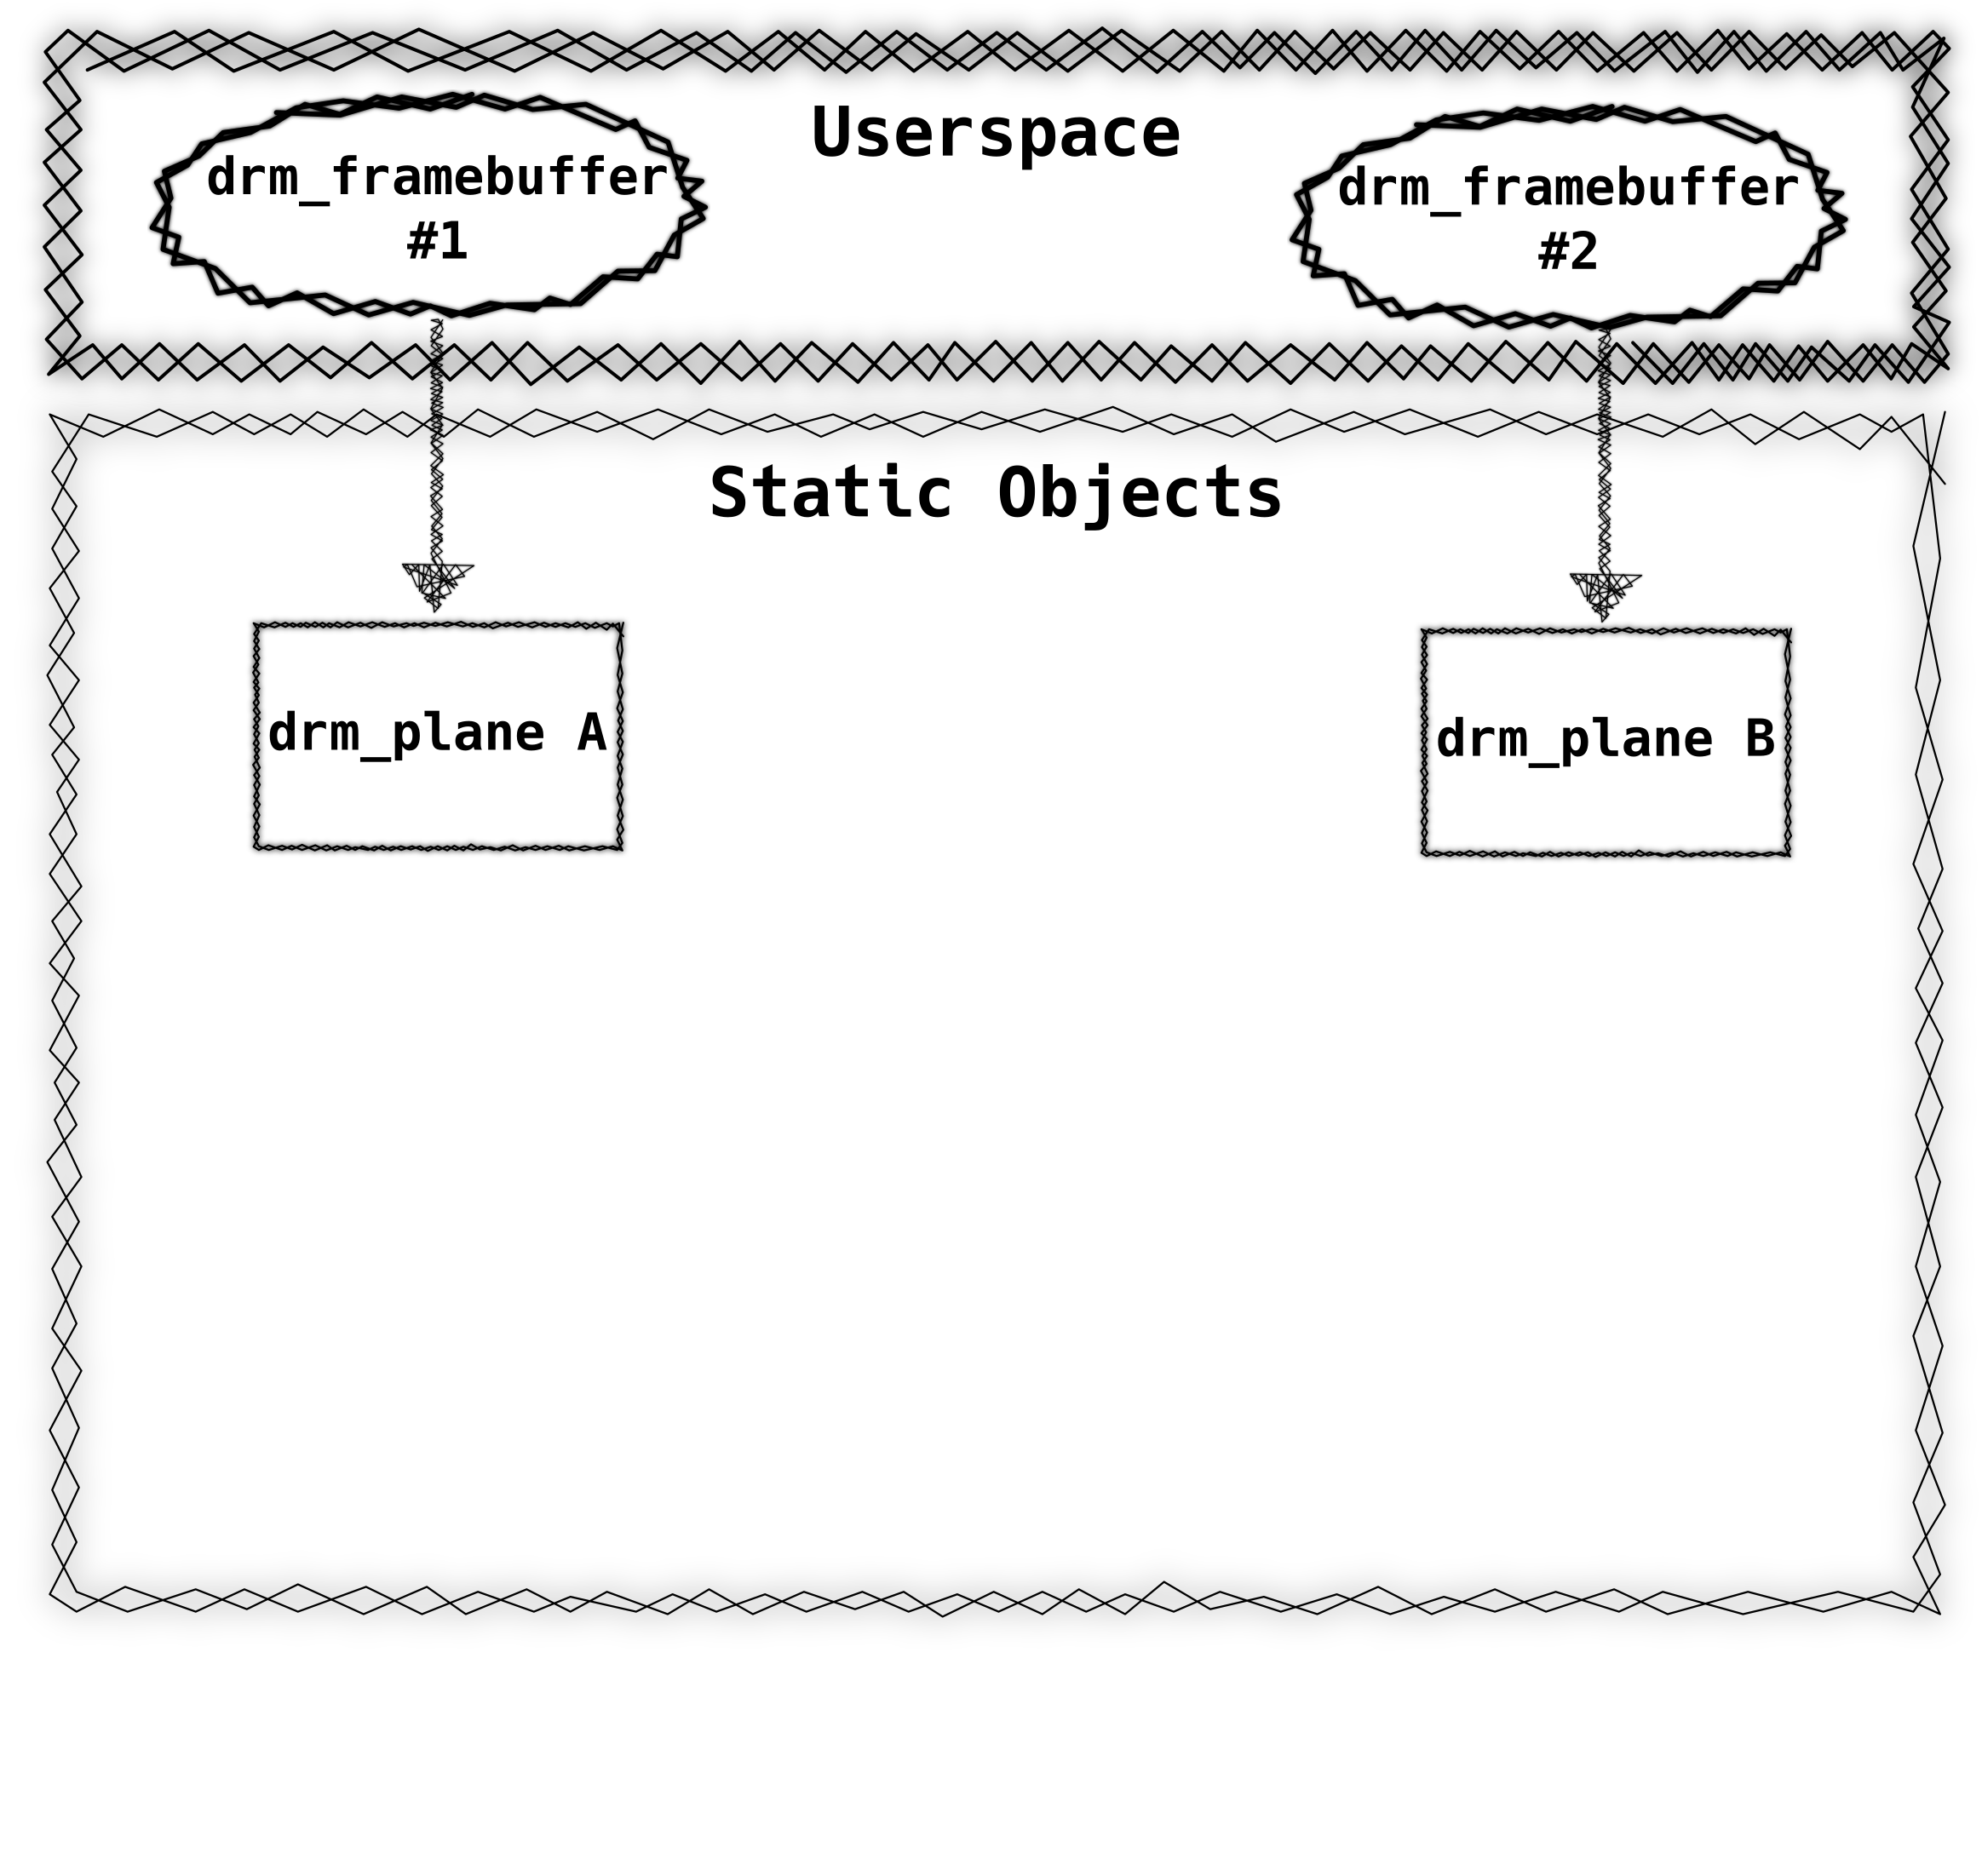
\includegraphics[width=\linewidth,
                     height=0.8\textheight,
                     keepaspectratio]{drm_internals_2}
  \end{figure}
\end{frame}

\begin{frame}{100 foot view}
  \begin{figure}
    \centering
    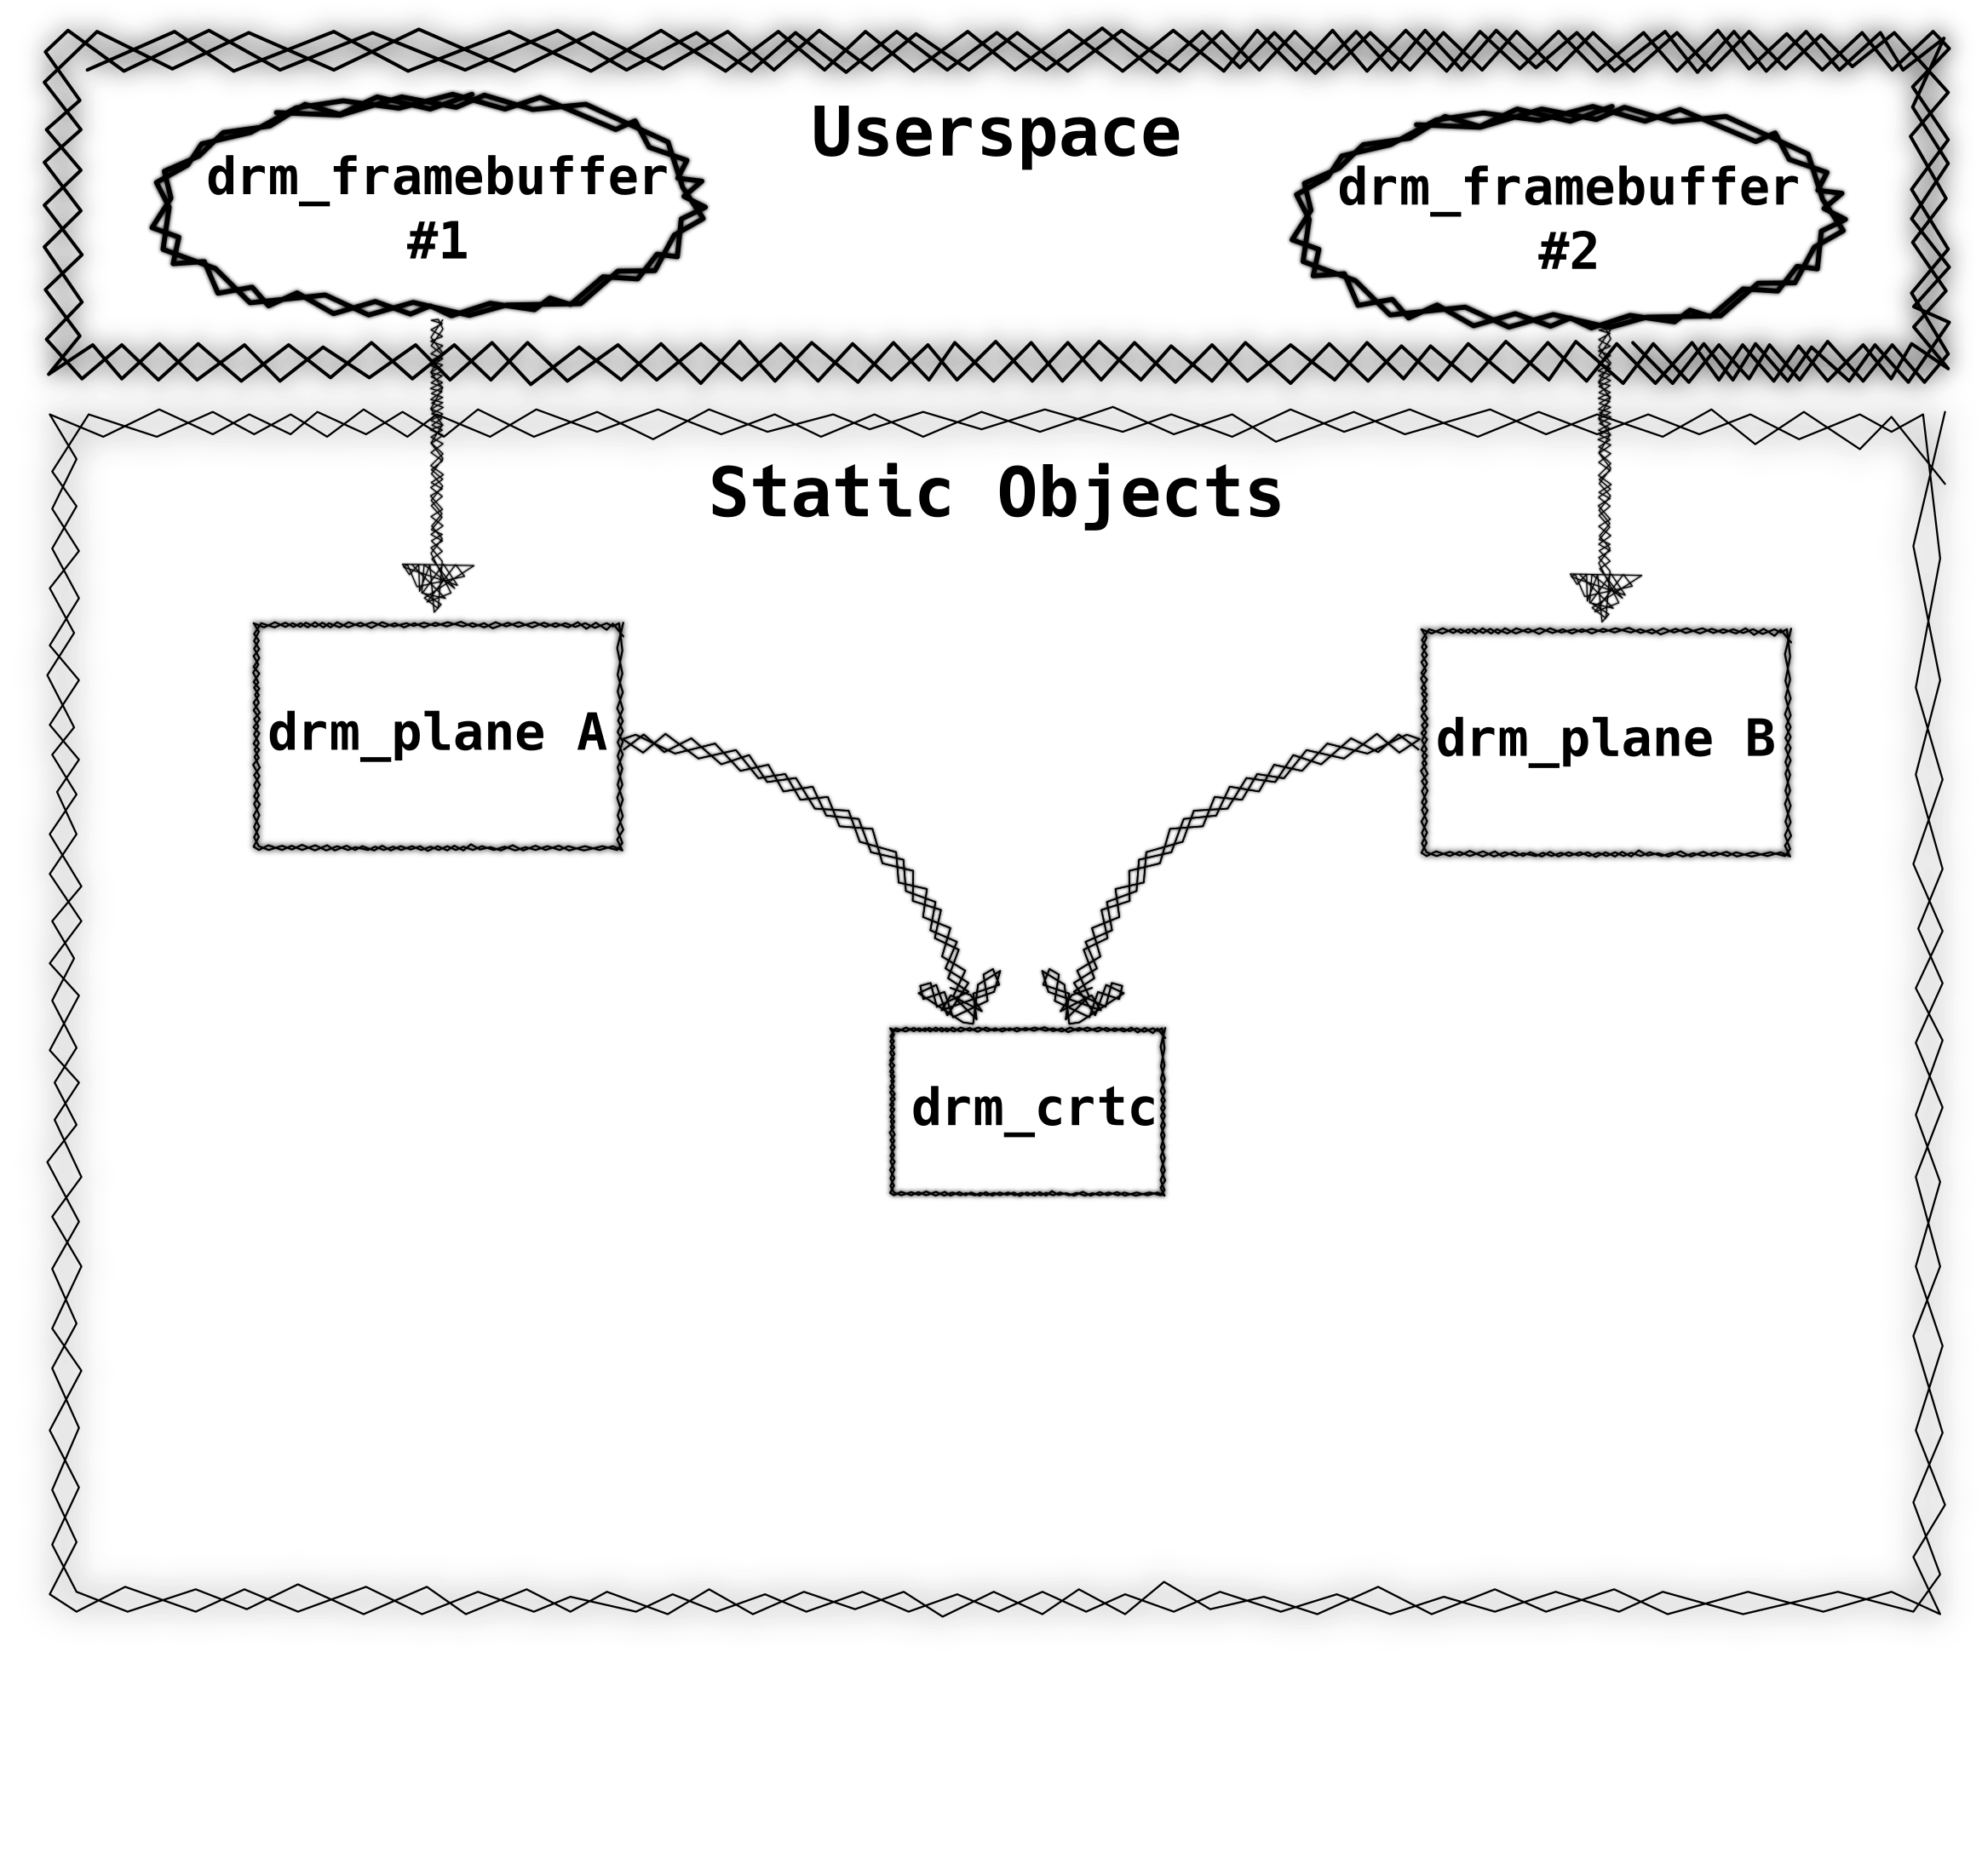
\includegraphics[width=\linewidth,
                     height=0.8\textheight,
                     keepaspectratio]{drm_internals_3-min}
  \end{figure}
\end{frame}

\begin{frame}{100 foot view}
  \begin{figure}
    \centering
    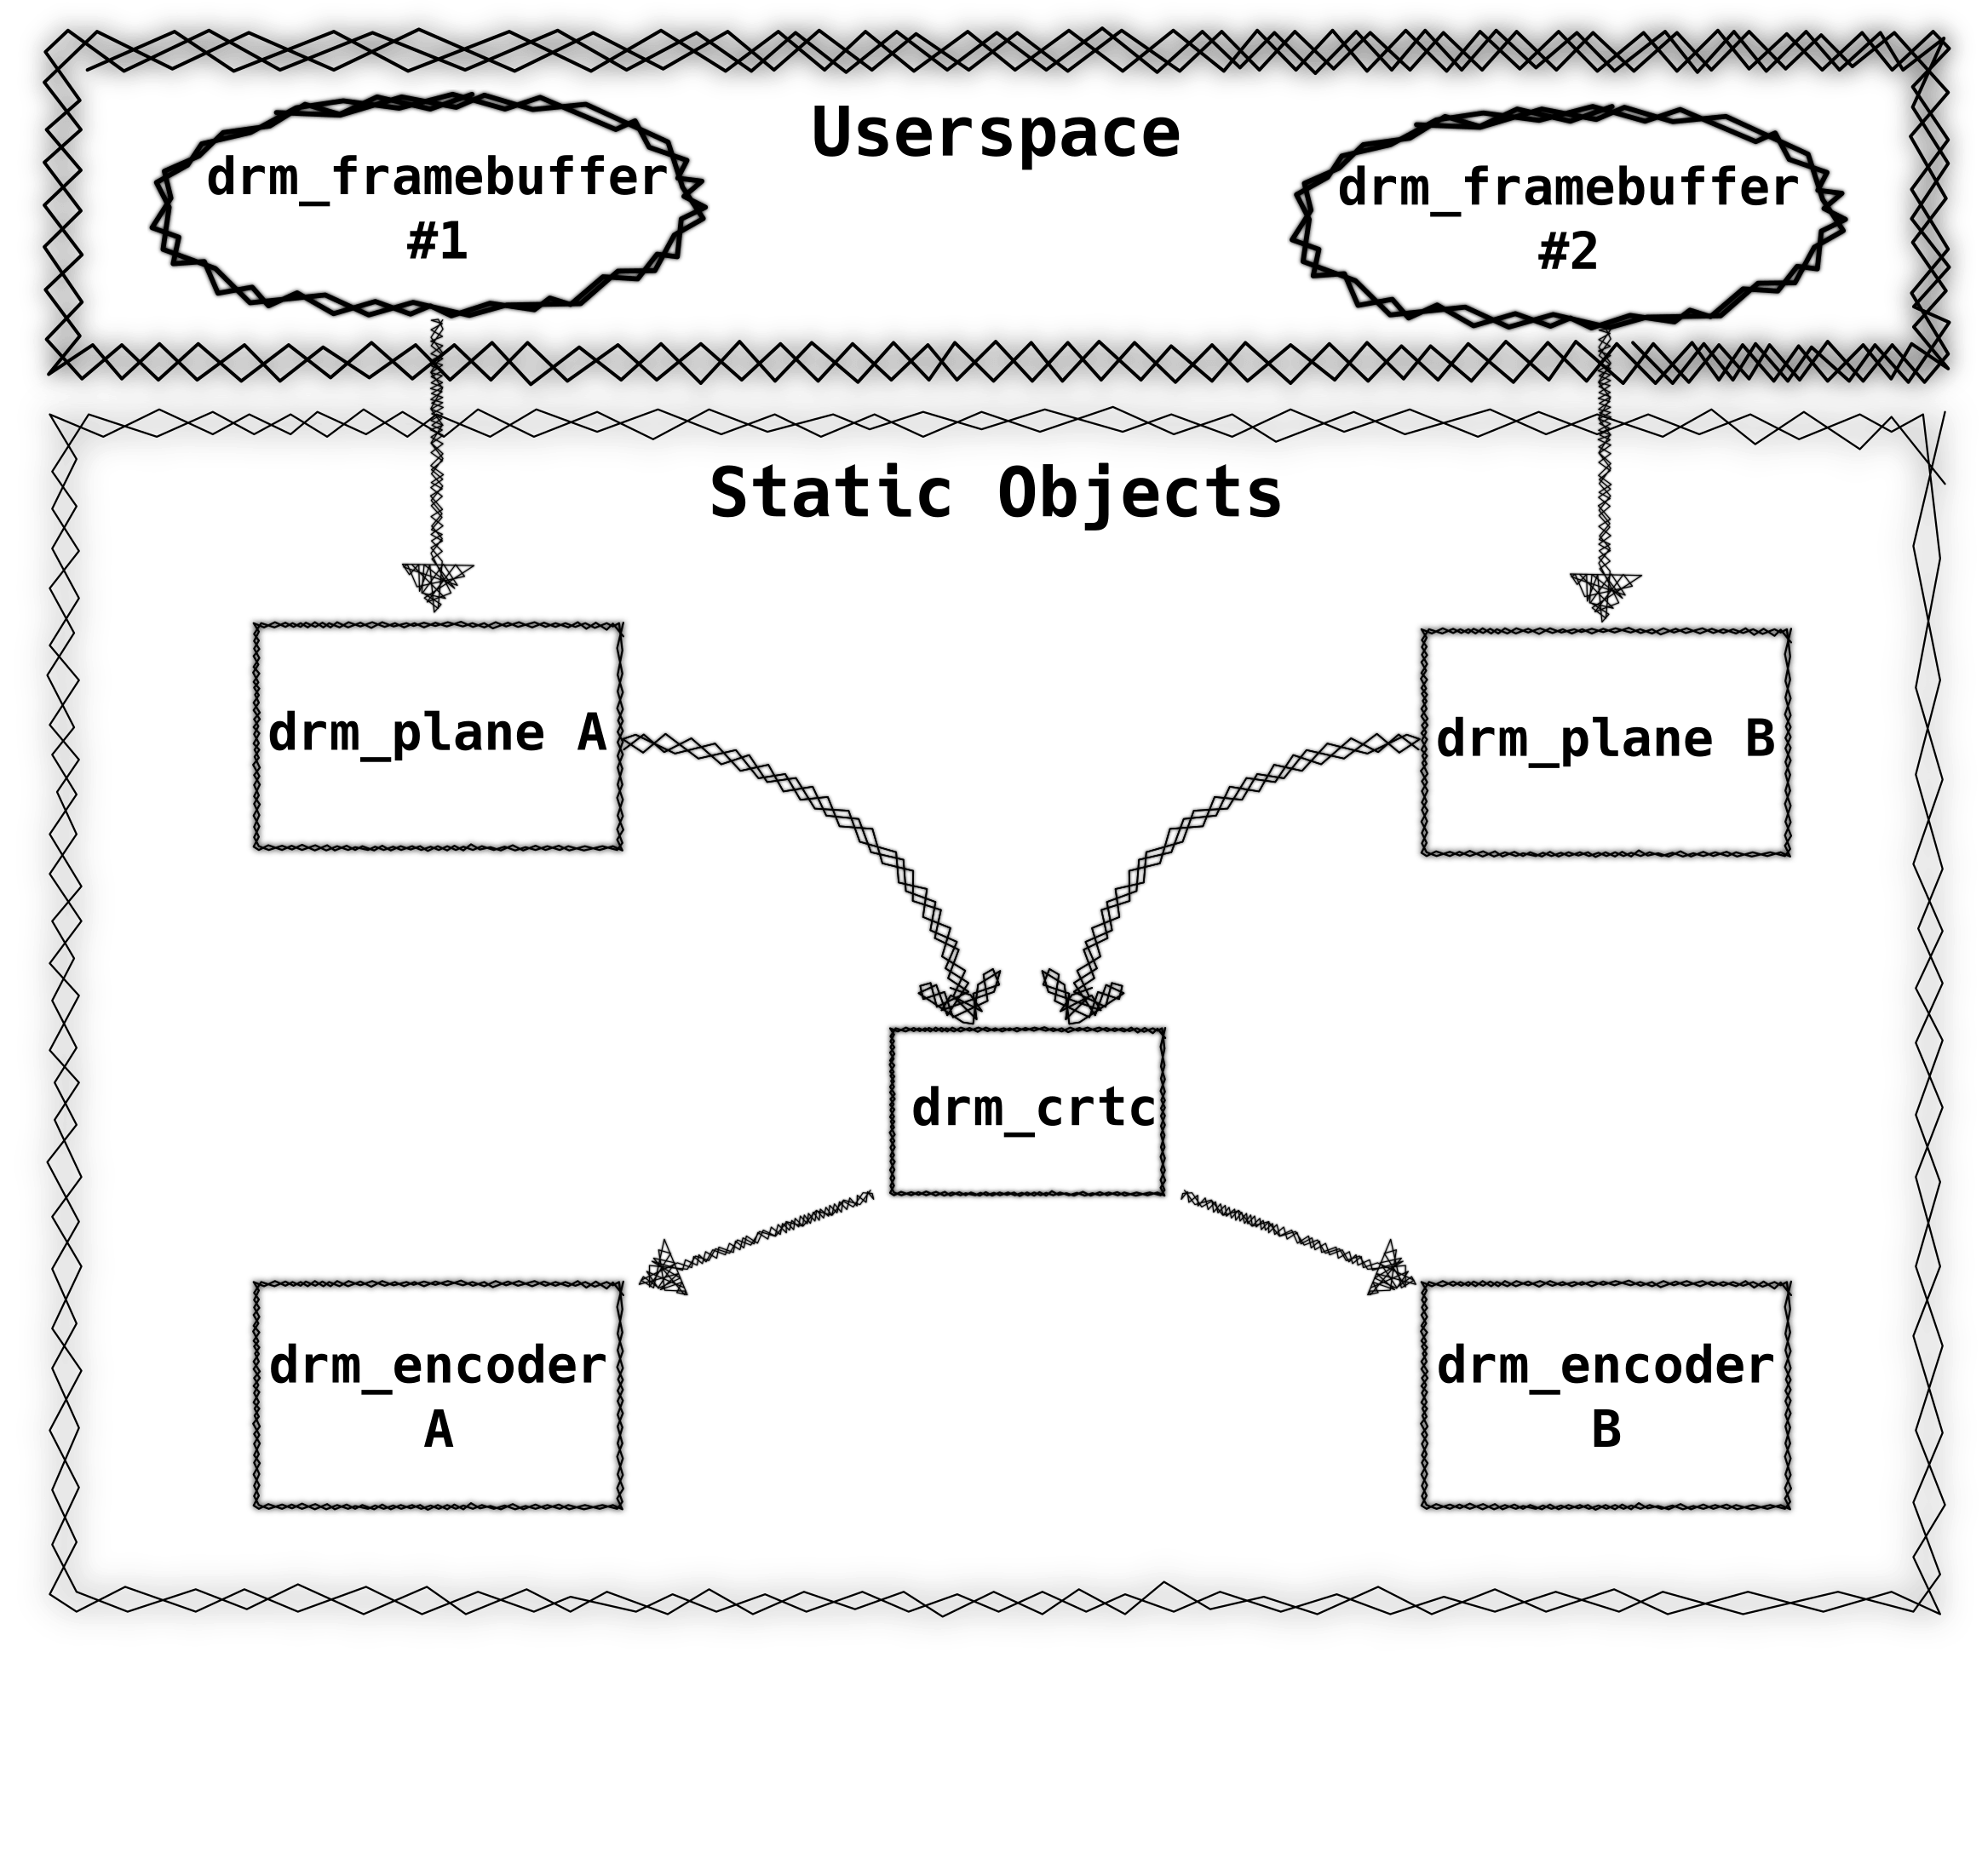
\includegraphics[width=\linewidth,
                     height=0.8\textheight,
                     keepaspectratio]{drm_internals_4-min}
  \end{figure}
\end{frame}

\begin{frame}{100 foot view}
  \begin{figure}
    \centering
    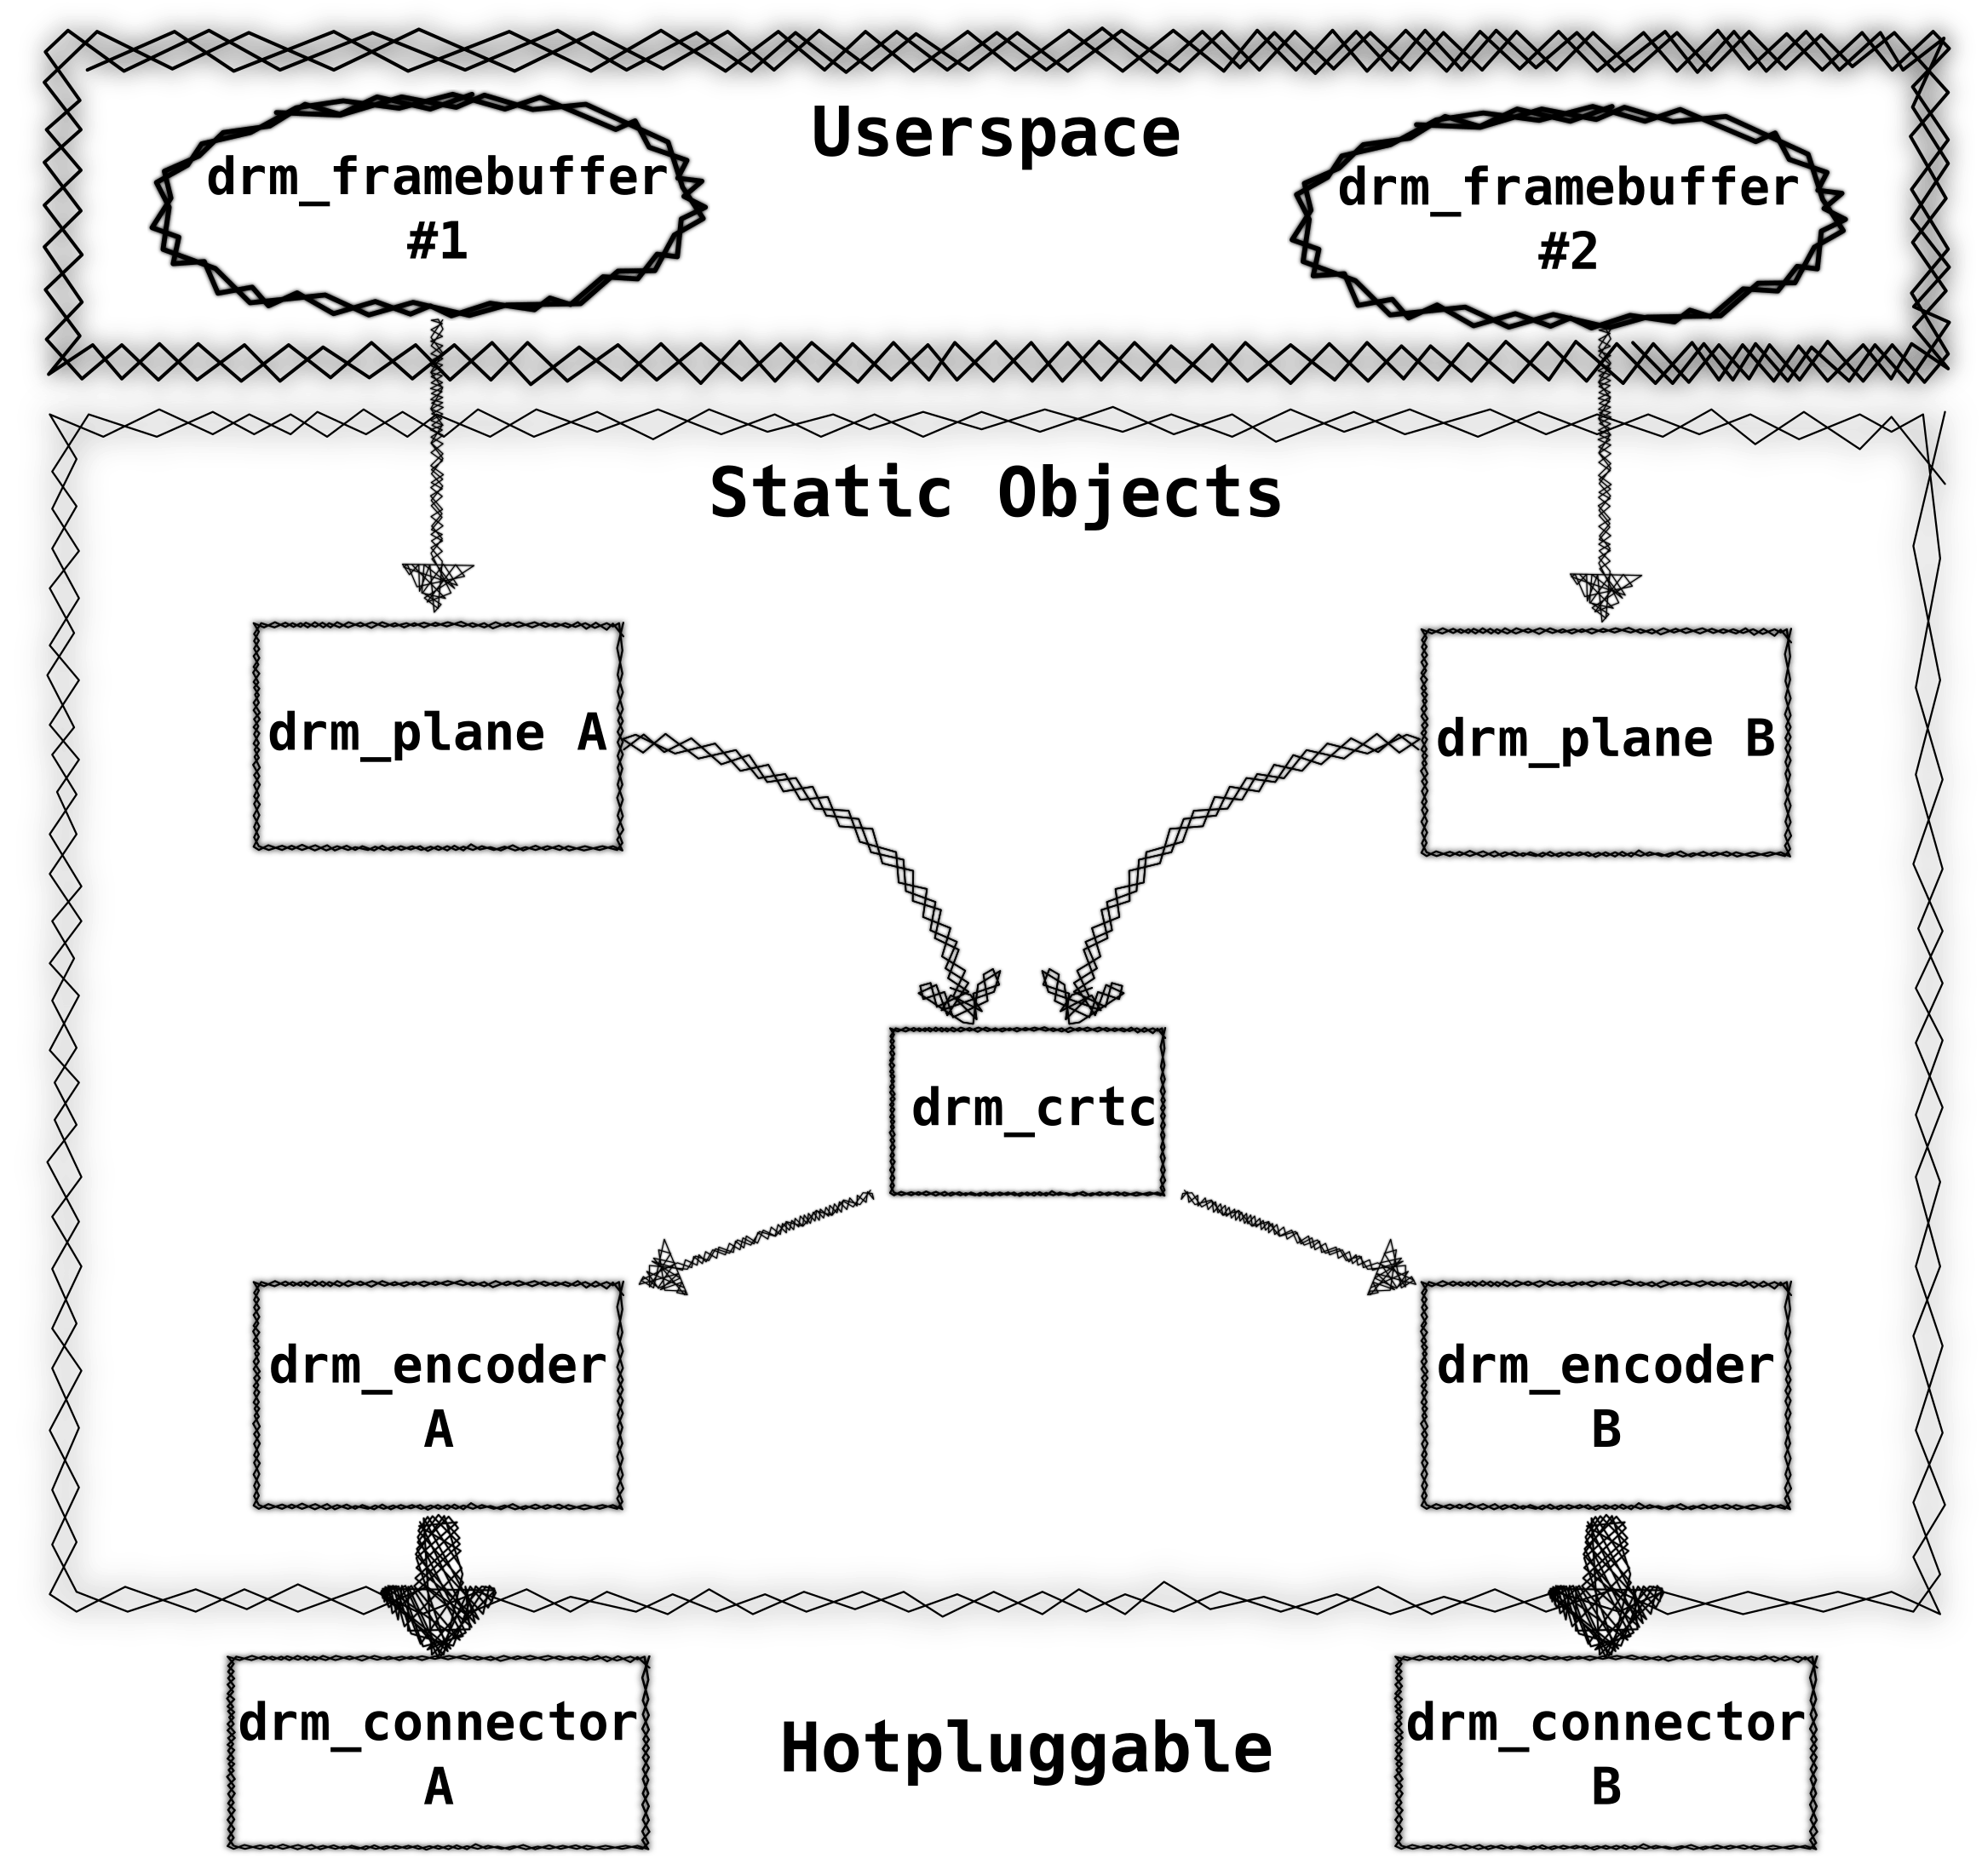
\includegraphics[width=\linewidth,
                     height=0.8\textheight,
                     keepaspectratio]{drm_internals-min}
  \end{figure}
\end{frame}

%------------------------------------------------------------------------------
\section{The Virtual Kernel Mode Setting (10 foot view)}

\begin{frame}{Virtual KMS}
  \metroset{block=fill}
  \begin{exampleblock}{About VKMS}
Creating a Virtual KMS (VKMS) has benefits. First, it could be used for
testing; second, it can be valuable for running X or Wayland on a headless
machine enabling the use of GPU. This module is similar to VGEM, and in some
ways to VIRTIO. At the moment that VKMS gets mature enough, it will be used to
run i-g-t test cases and to automate userspace testing.
  \end{exampleblock}
\end{frame}


\begin{frame}{About VKMS}
  General Info:
  \begin{itemize}
    \item Developers: Haneen Mohammed and Rodrigo Siqueira
    \item Mentors: Daniel Vetter, Gustavo Padovan, and Sean Paul
  \end{itemize}
  Some of the VKMS features:
  \begin{itemize}
    \item Dumb memory
    \item CRTC, Virtual Encoder and Connector
    \item Two operation mode: With and without VBlank
    \item CRC validation
  \end{itemize}
\end{frame}

\section{1 foot view}

\begin{frame}{The problem}
  \begin{figure}
    \centering
    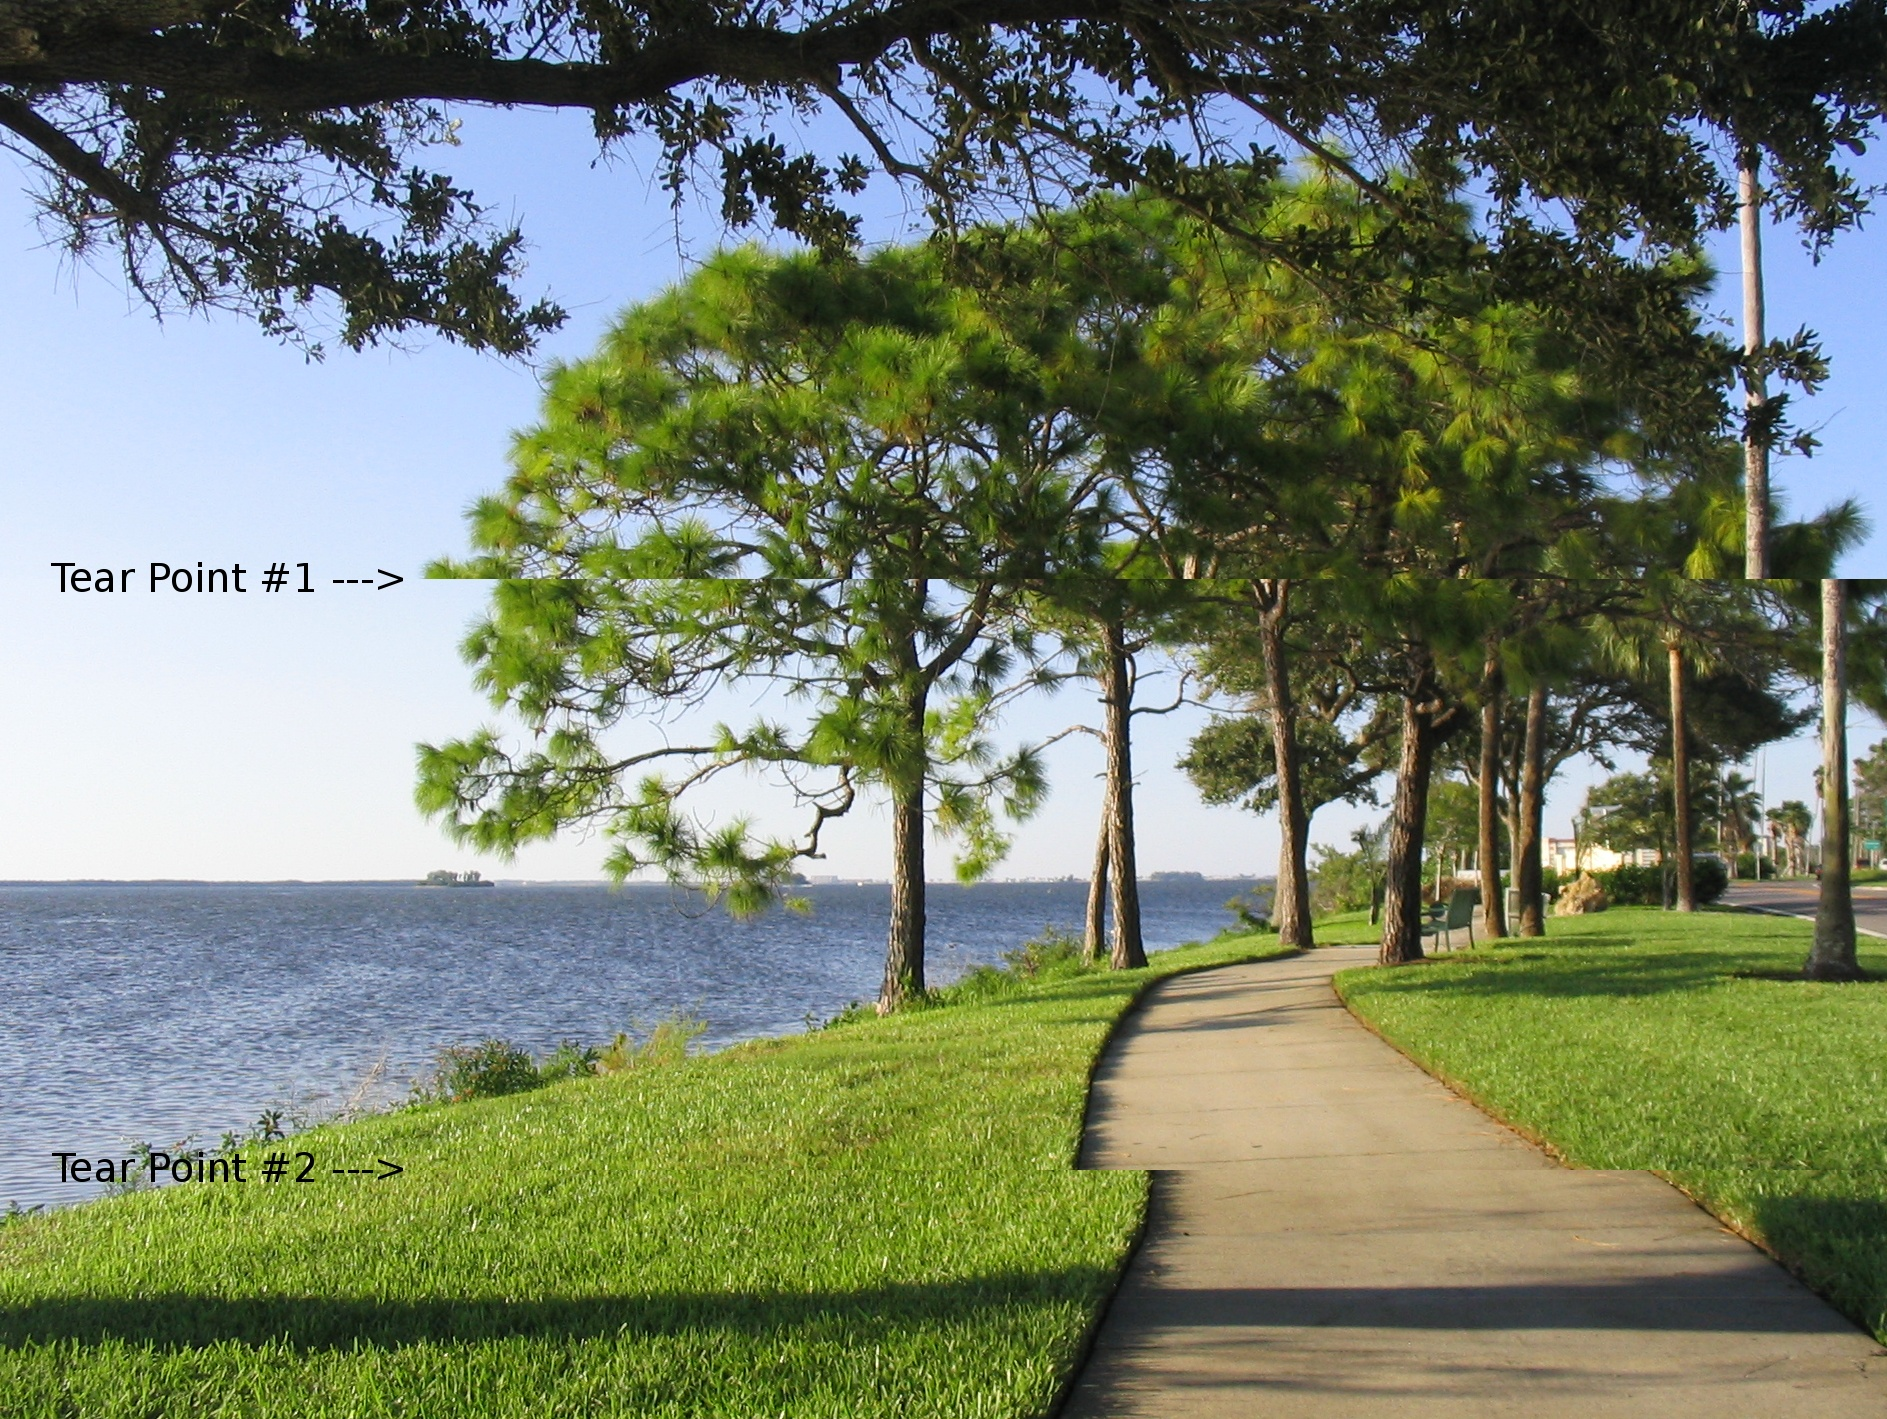
\includegraphics[width=\linewidth,
                     height=0.9\textheight,
                     keepaspectratio]{tearing}
  \end{figure}
\end{frame}

\begin{frame}{Page-Flip}
  \begin{figure}
    \centering
    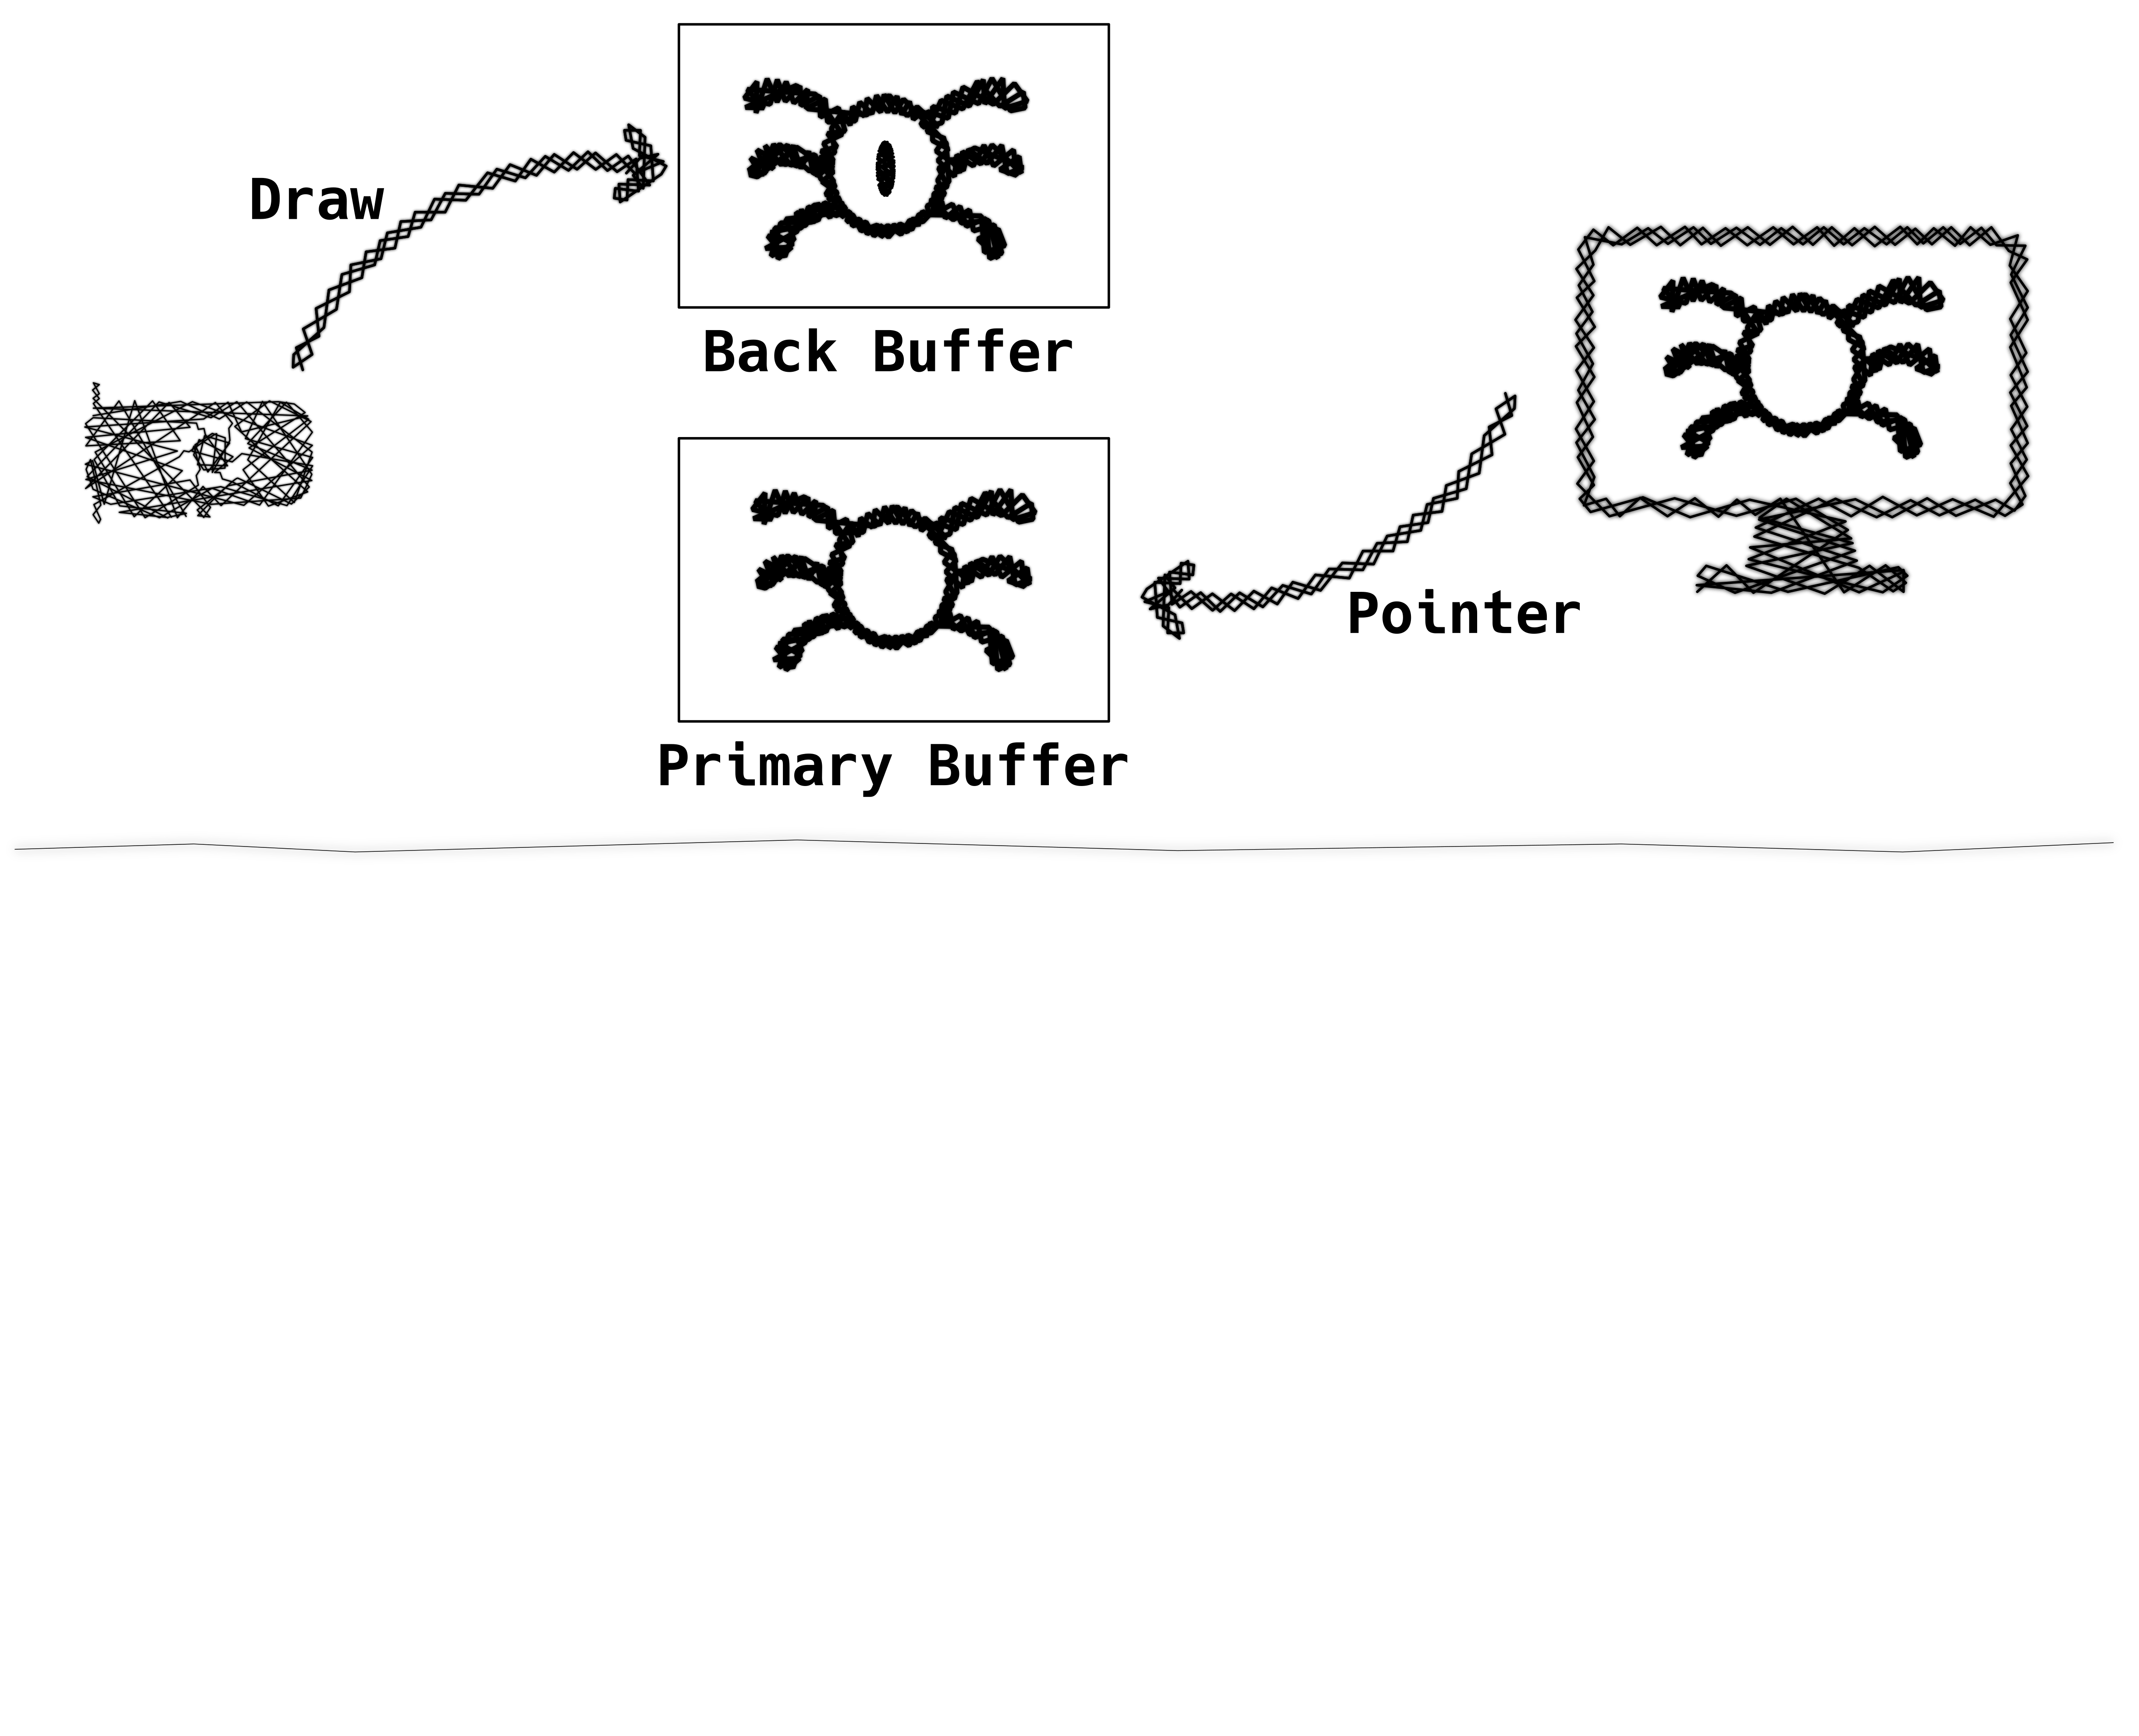
\includegraphics[width=\linewidth,
                     height=0.8\textheight,
                     keepaspectratio]{page-flip_1-min}
  \end{figure}
\end{frame}

\begin{frame}{Page-Flip}
  \begin{figure}
    \centering
    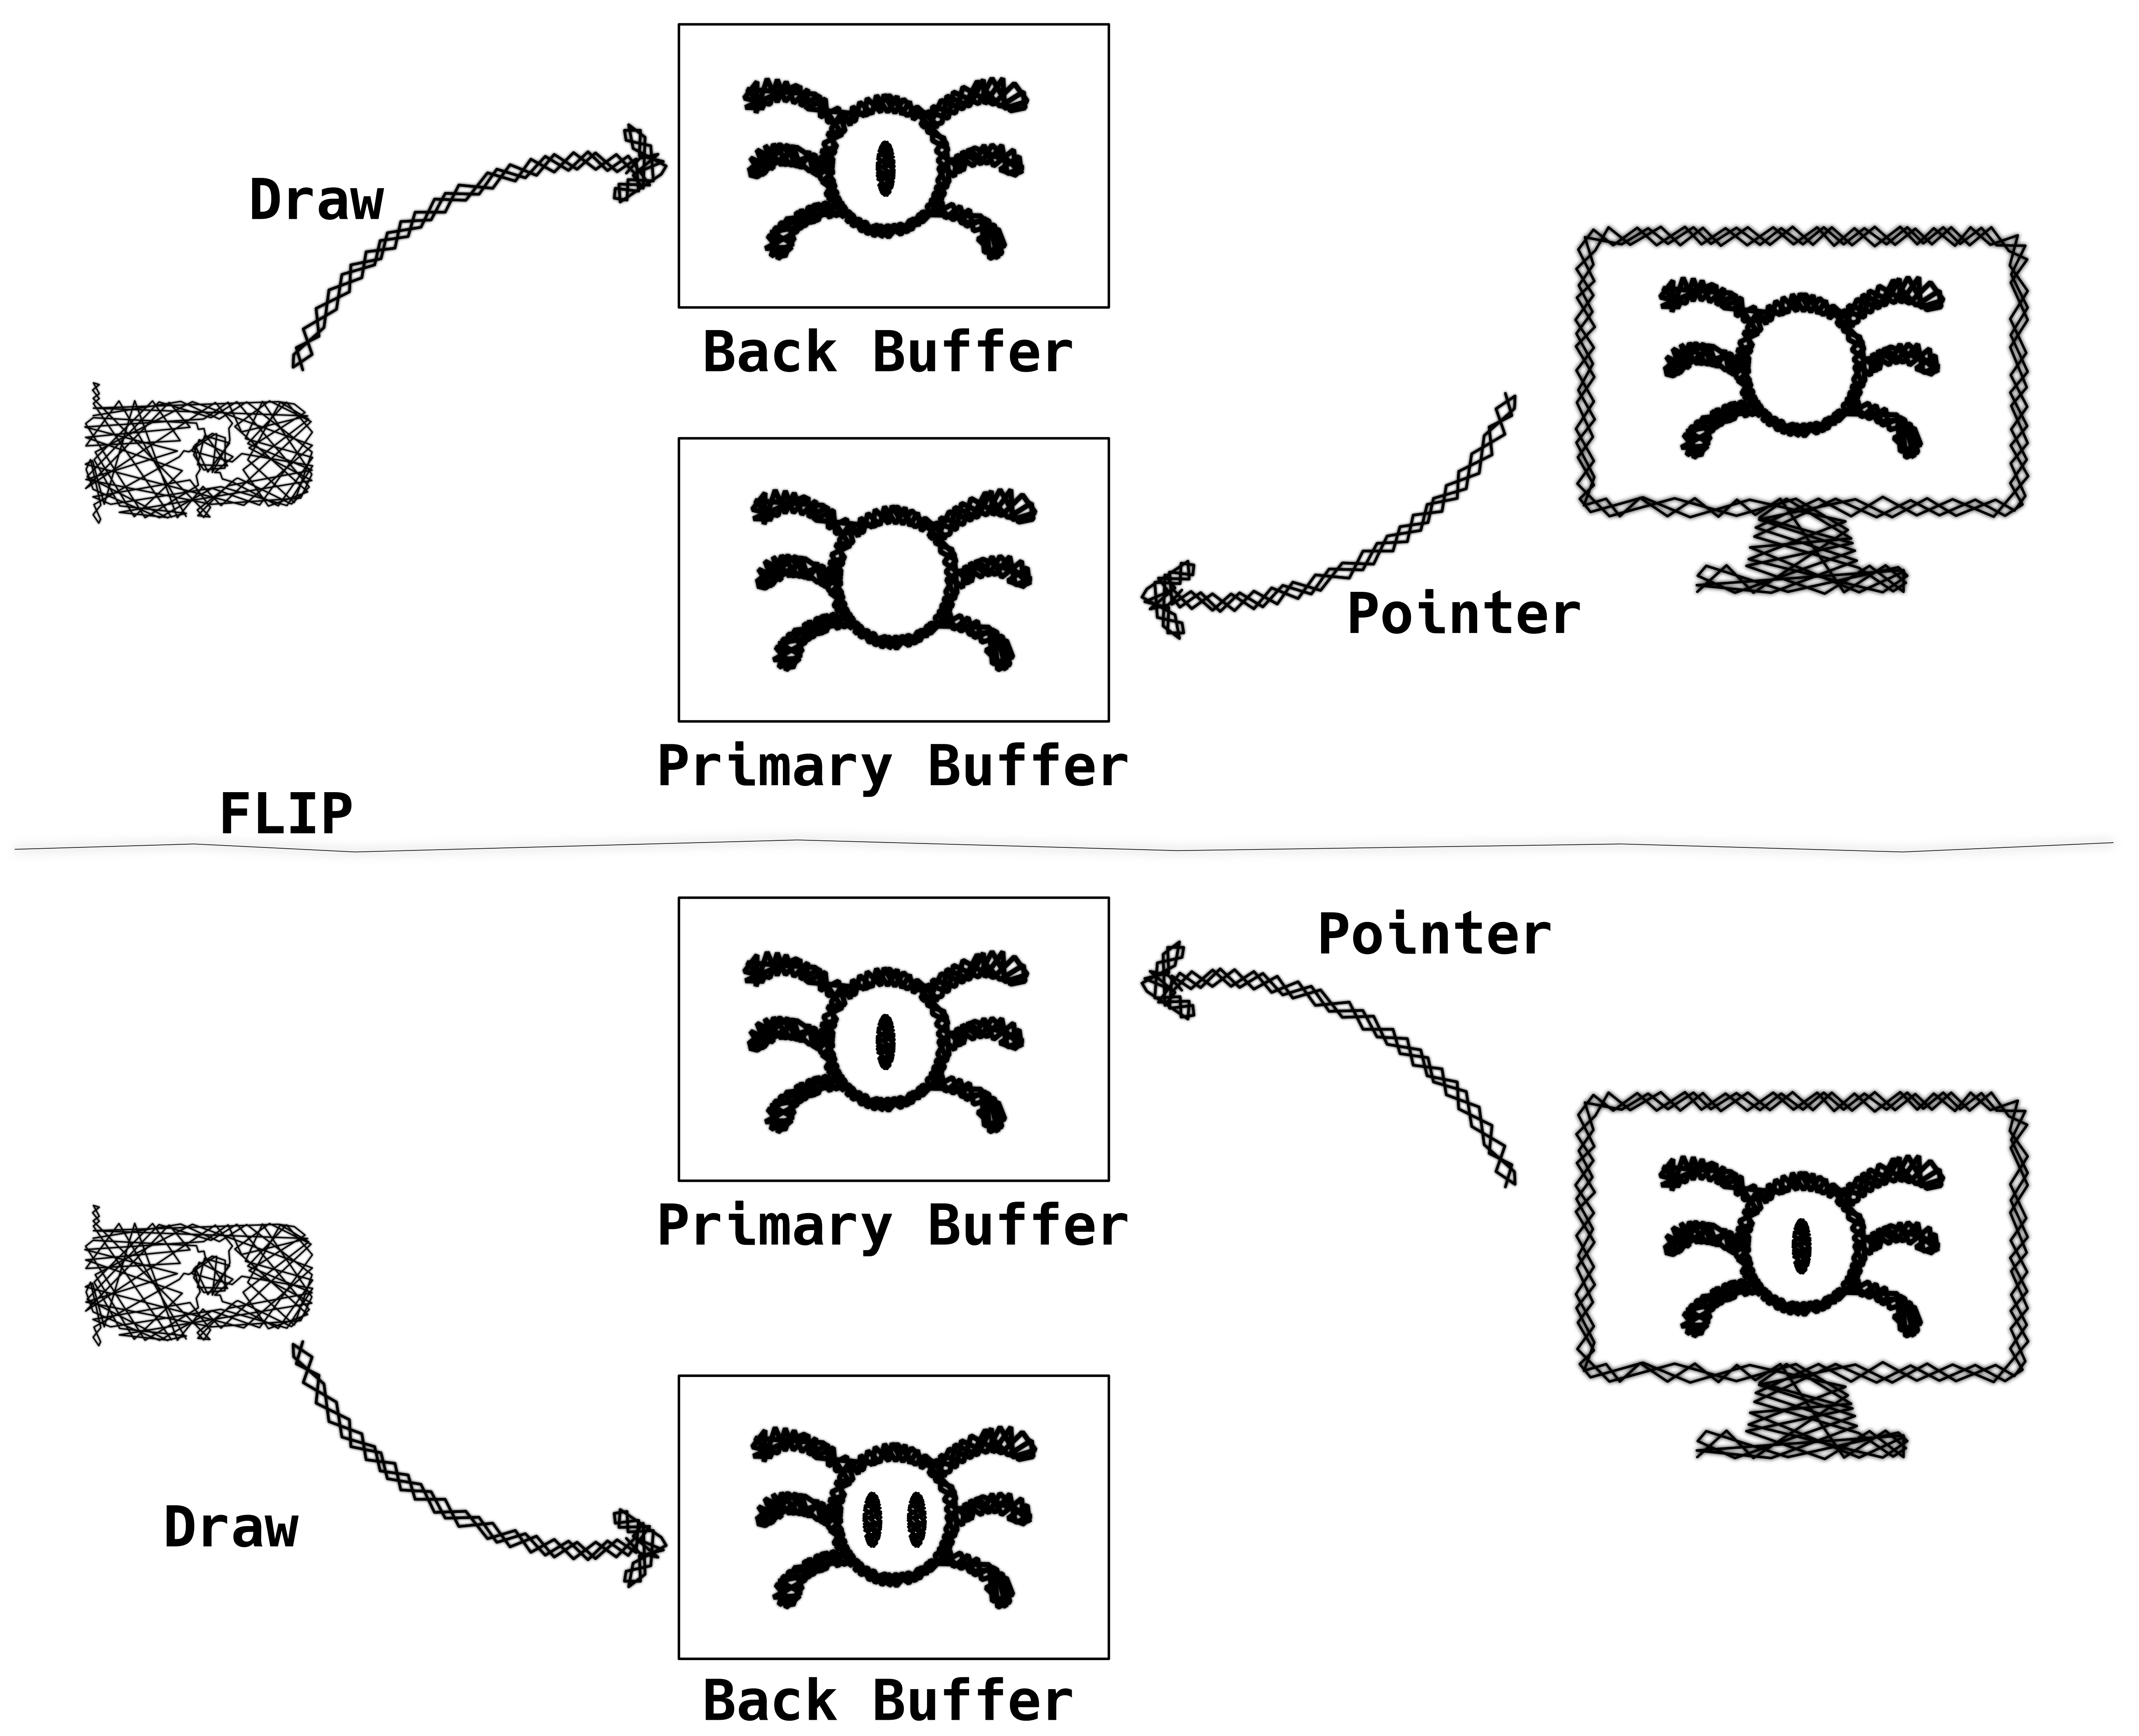
\includegraphics[width=\linewidth,
                     height=0.8\textheight,
                     keepaspectratio]{page-flip-min}
  \end{figure}
\end{frame}

\begin{frame}{VKMS TDD}
  \begin{figure}
    \centering
    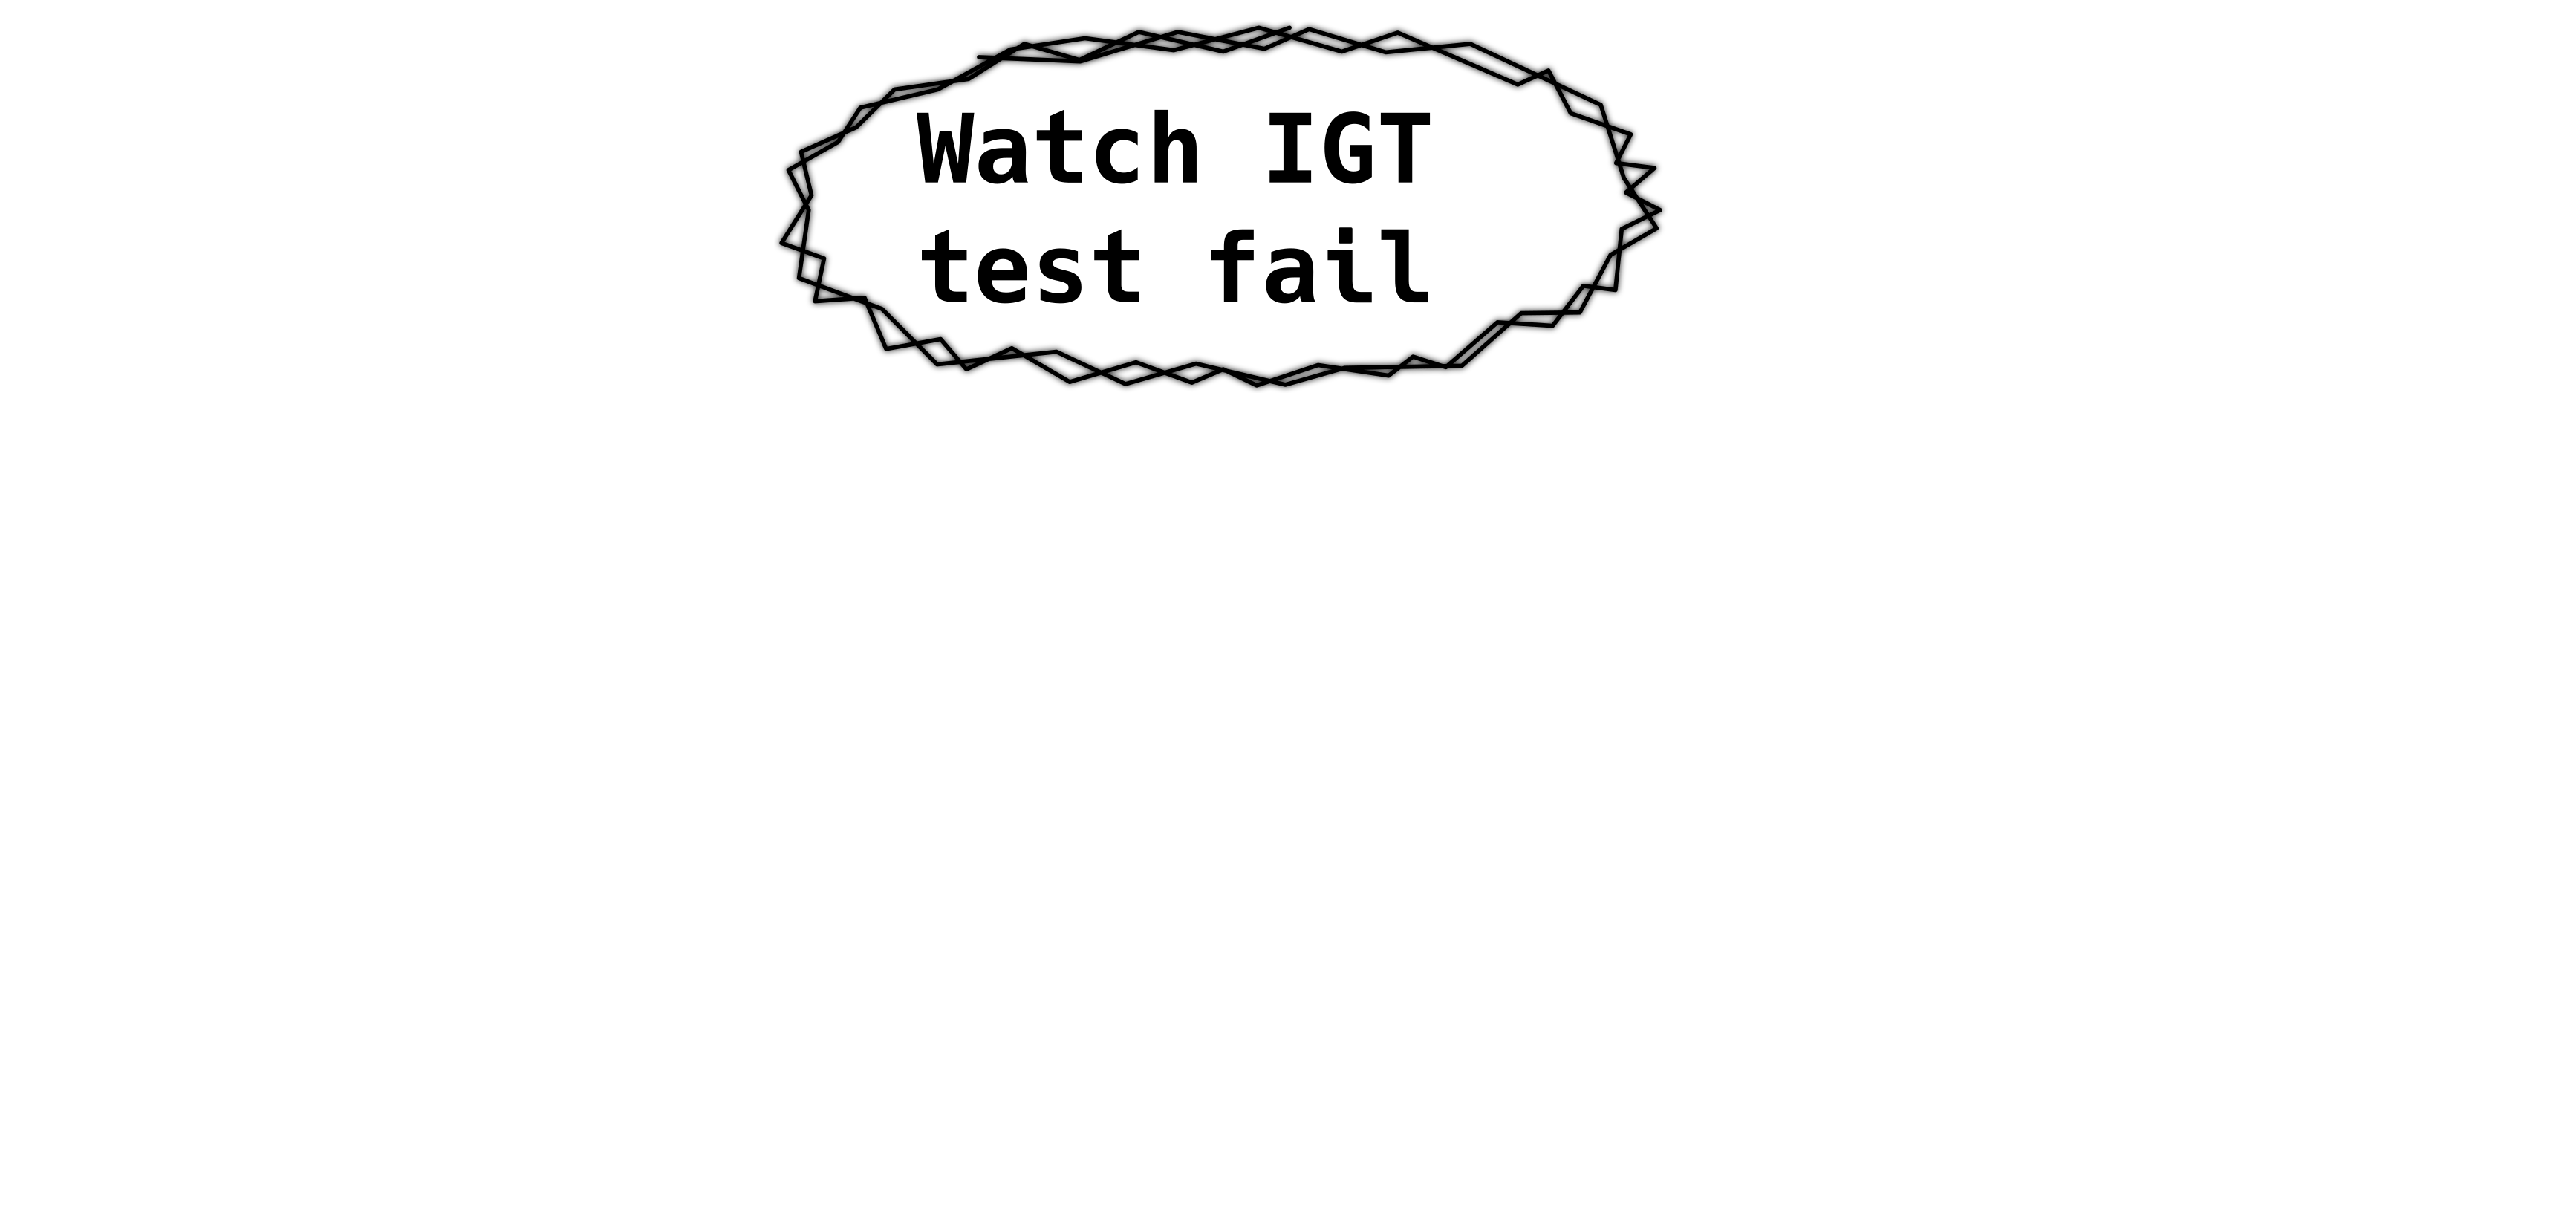
\includegraphics[width=\linewidth,
                     height=0.8\textheight,
                     keepaspectratio]{tdd-drm_1}
  \end{figure}
\end{frame}

\begin{frame}{VKMS TDD}
  \begin{figure}
    \centering
    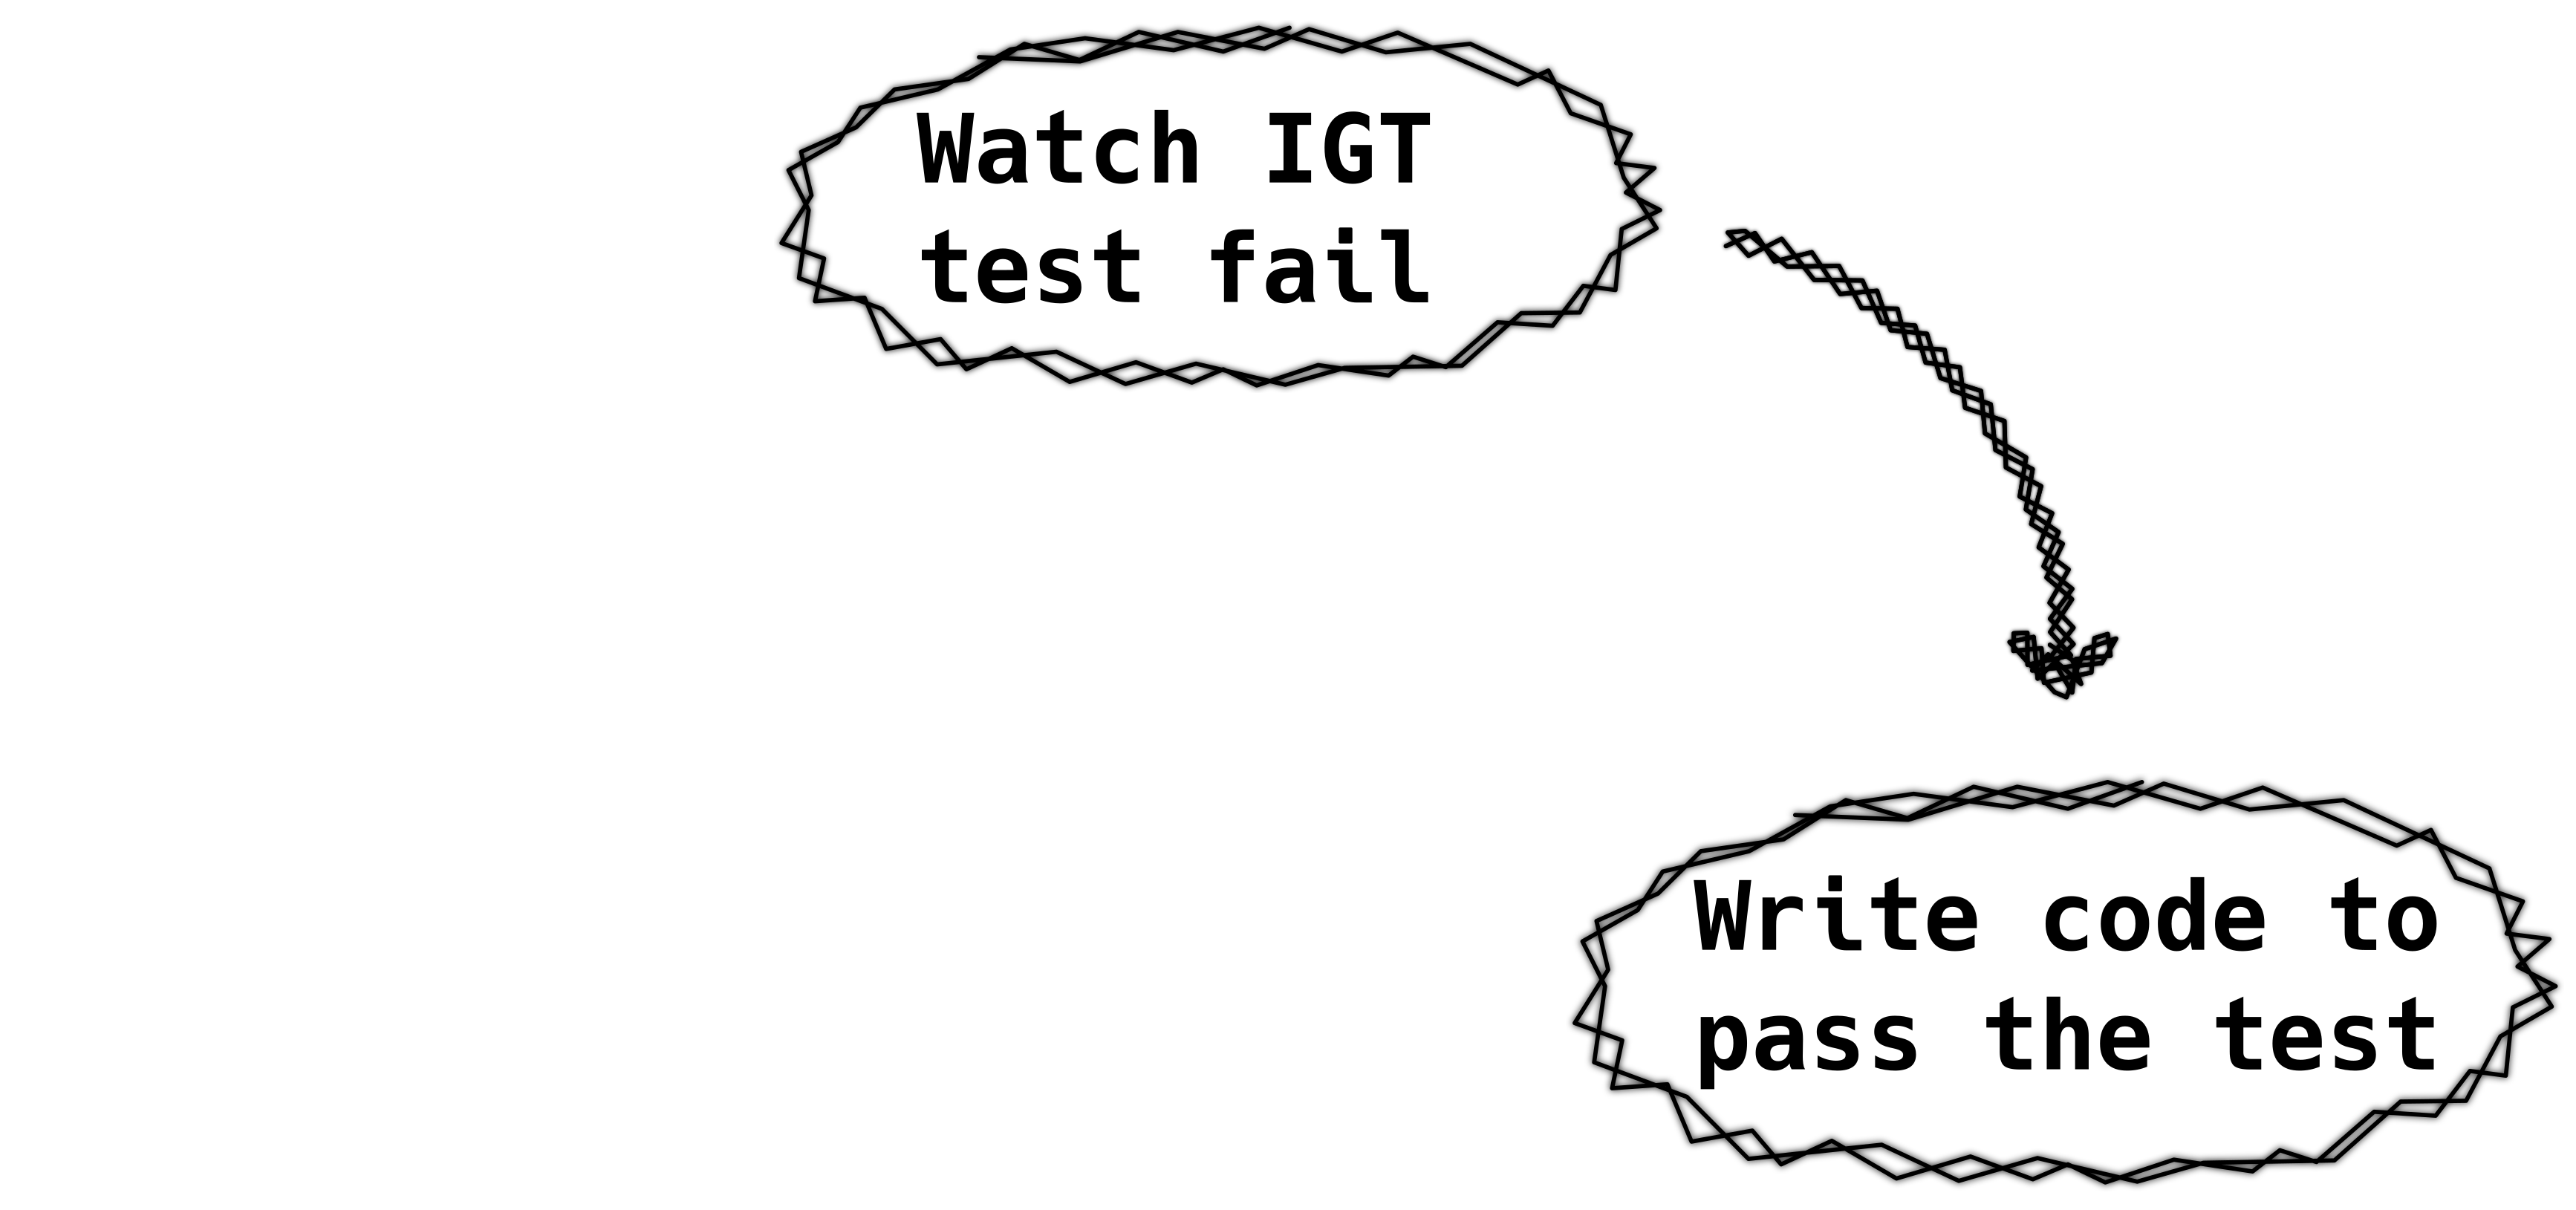
\includegraphics[width=\linewidth,
                     height=0.8\textheight,
                     keepaspectratio]{tdd-drm_2}
  \end{figure}
\end{frame}

\begin{frame}{VKMS TDD}
  \begin{figure}
    \centering
    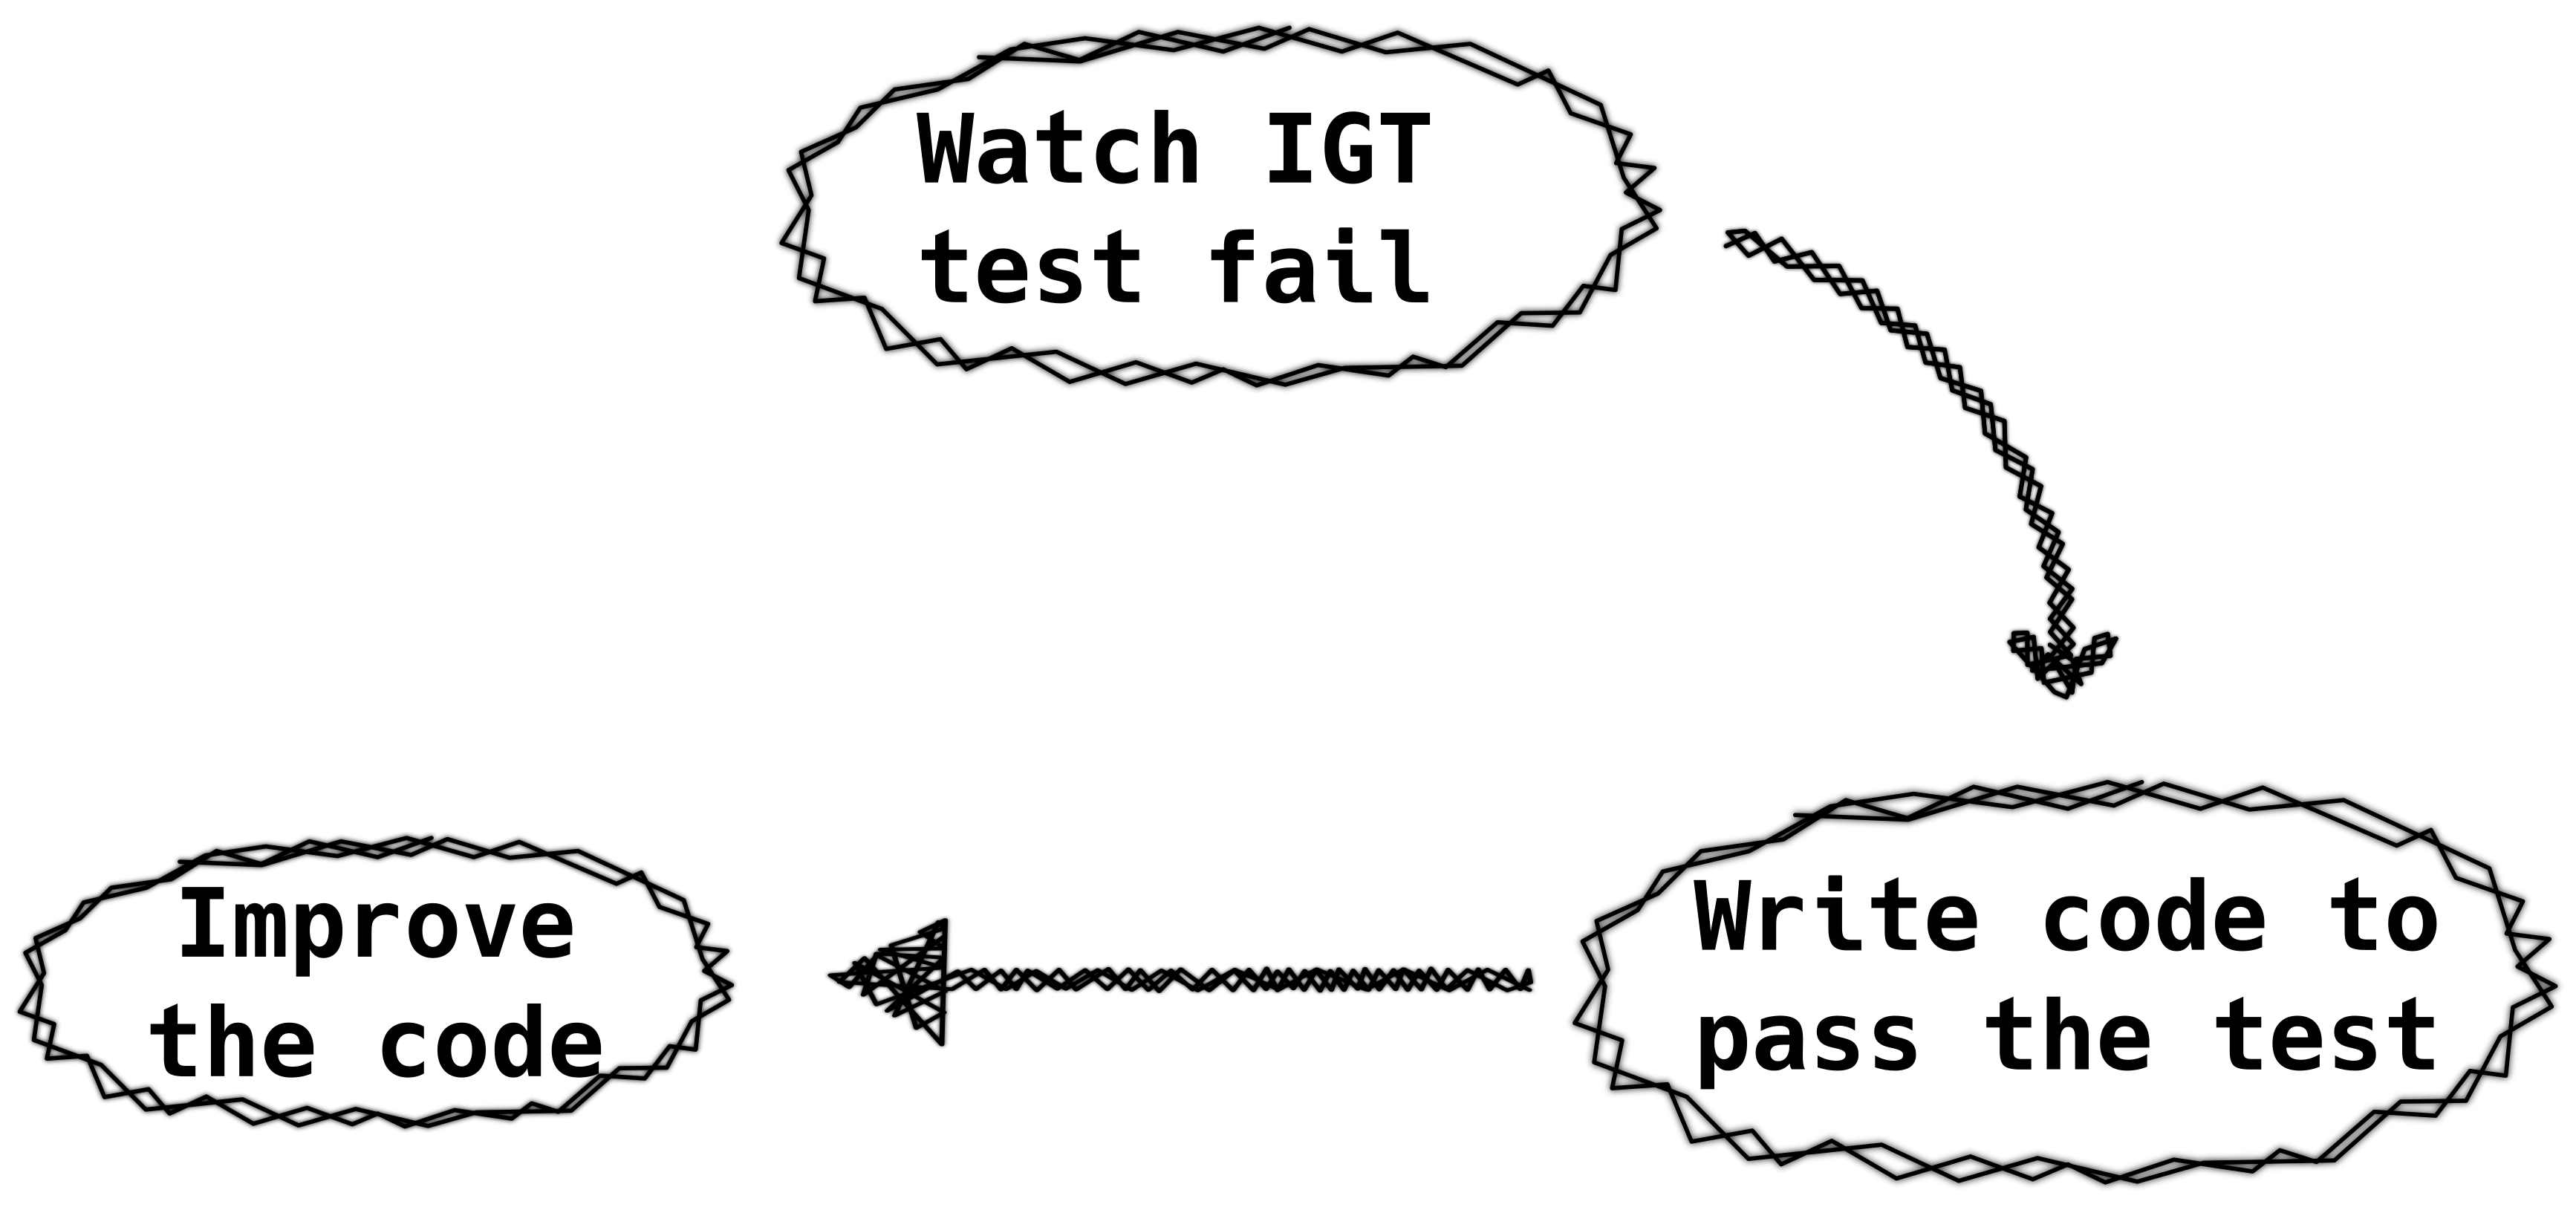
\includegraphics[width=\linewidth,
                     height=0.8\textheight,
                     keepaspectratio]{tdd-drm_3}
  \end{figure}
\end{frame}

\begin{frame}{VKMS TDD}
  \begin{figure}
    \centering
    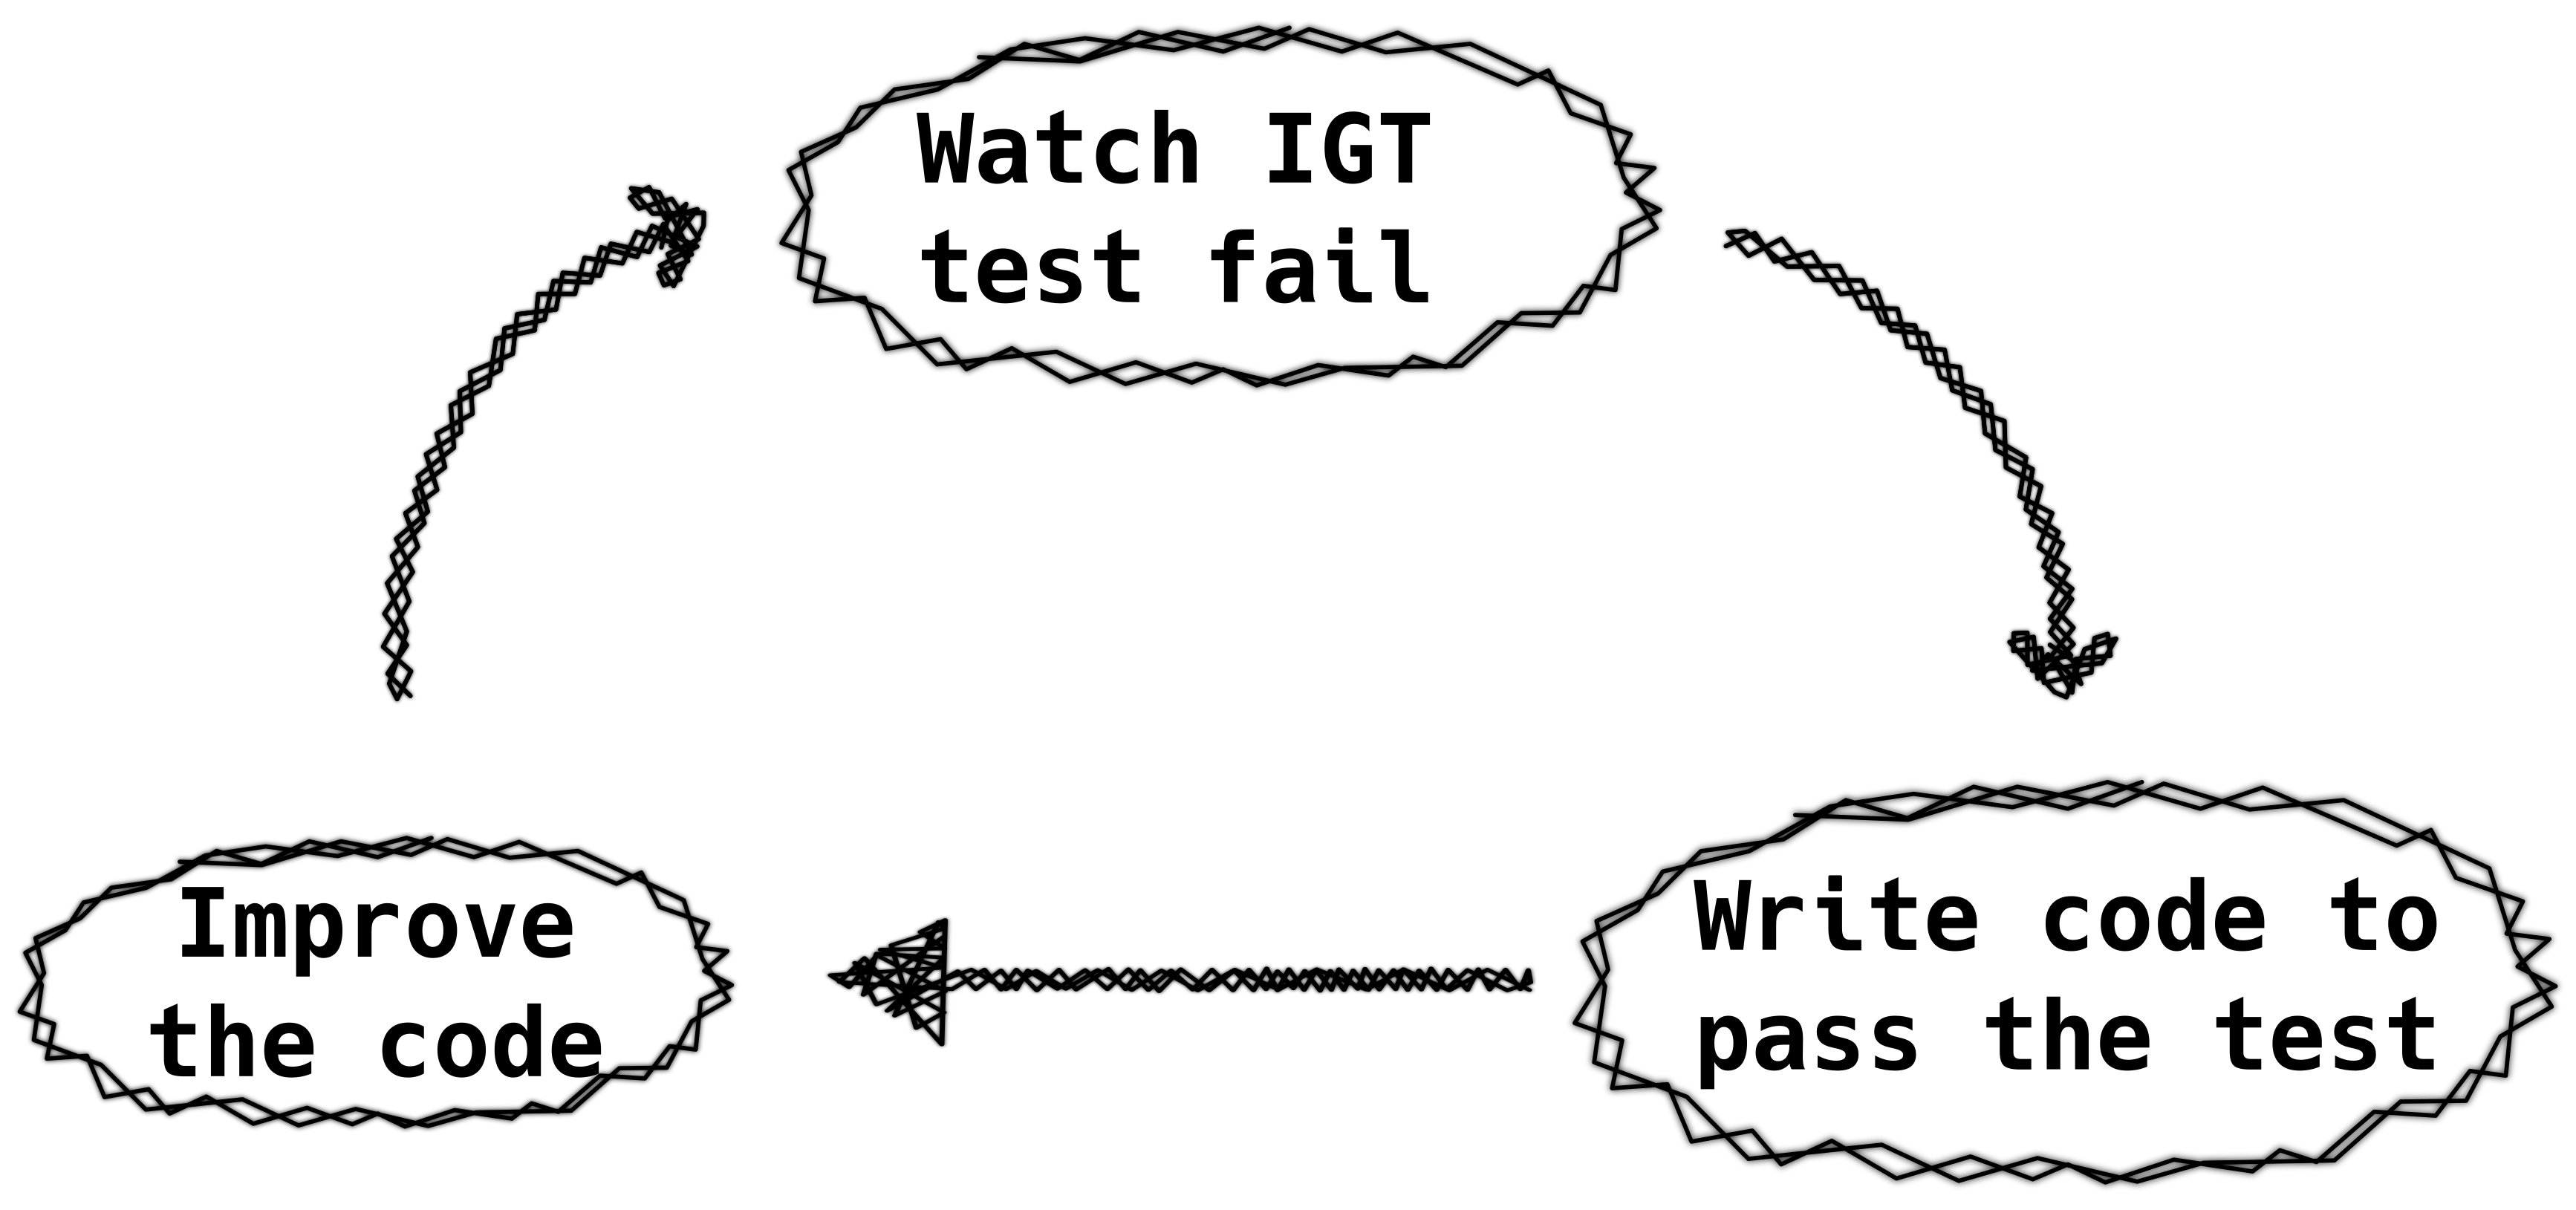
\includegraphics[width=\linewidth,
                     height=0.8\textheight,
                     keepaspectratio]{tdd-drm}
  \end{figure}
\end{frame}

\begin{frame}{Result 1}
  \begin{figure}
    \centering
    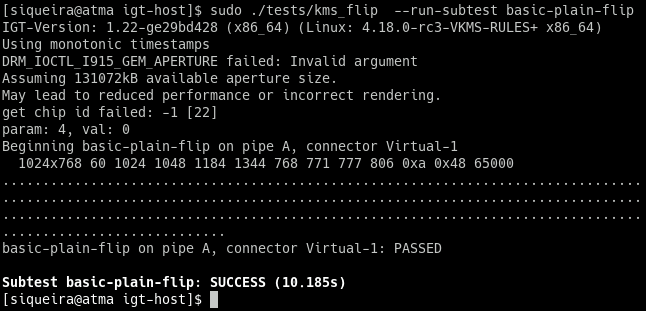
\includegraphics[width=\linewidth,
                     height=0.8\textheight,
                     keepaspectratio]{basic-plain-flip_passing}
  \end{figure}
\end{frame}

\begin{frame}{Result 2}
  \begin{figure}
    \centering
    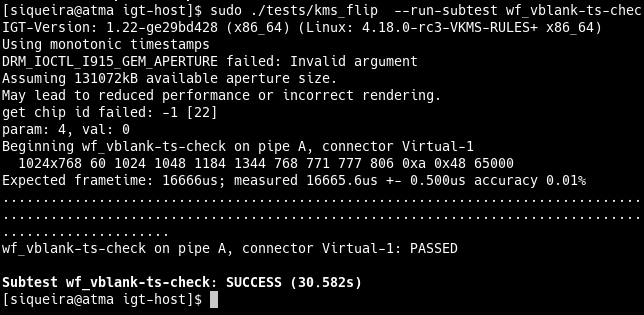
\includegraphics[width=\linewidth,
                     height=0.8\textheight,
                     keepaspectratio]{wf_vblank-ts-check}
  \end{figure}
\end{frame}

%------------------------------------------------------------------------------
\section{Linuxdev-br 2017 e GSoC 2018}
\begin{frame}{Linuxdev-br 2017}
  \begin{figure}
    \centering
    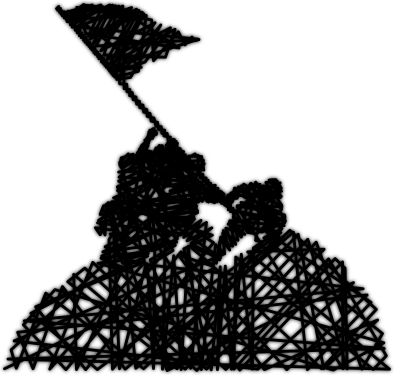
\includegraphics[width=\linewidth,
                     height=0.8\textheight,
                     keepaspectratio]{together}
  \end{figure}
\end{frame}

\begin{frame}{GSoC}
  \begin{figure}
    \centering
    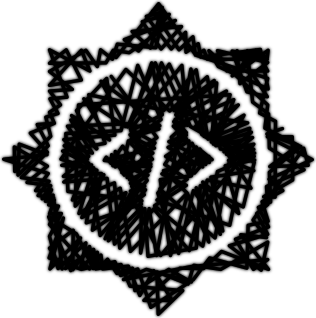
\includegraphics[width=\linewidth,
                     height=0.8\textheight,
                     keepaspectratio]{gsoc}
  \end{figure}
\end{frame}

\begin{frame}{GSoC}
  \begin{figure}
    \centering
    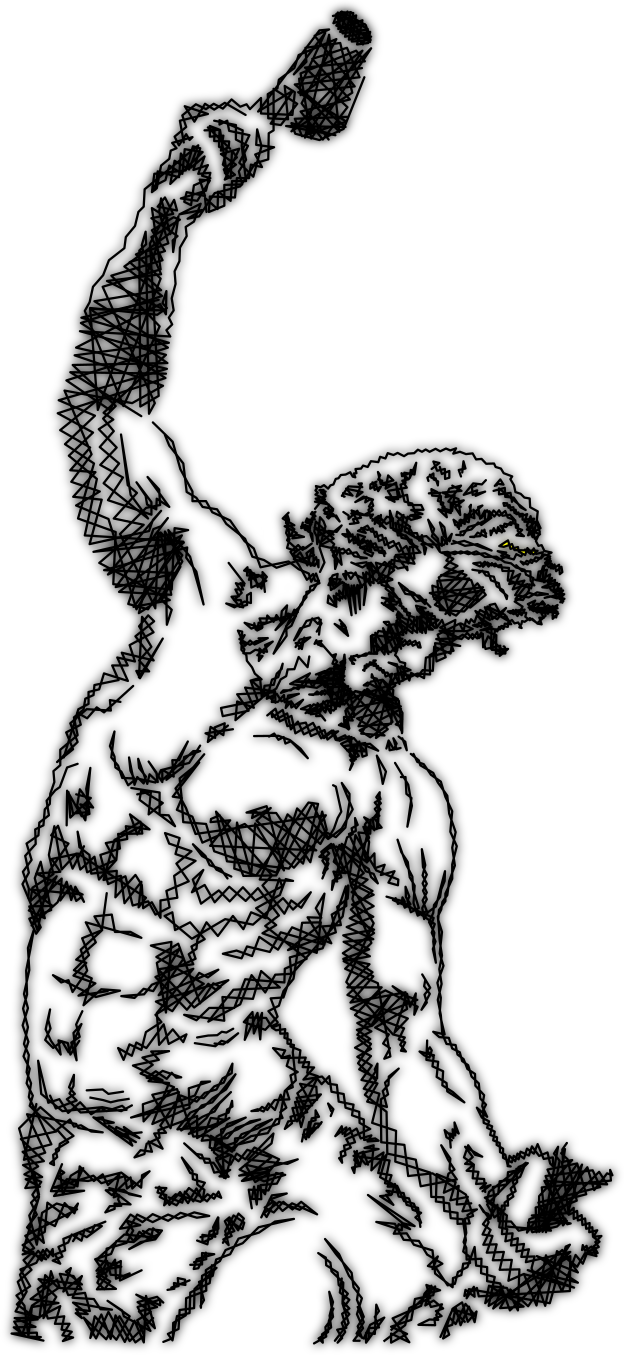
\includegraphics[width=\linewidth,
                     height=0.8\textheight,
                     keepaspectratio]{self_made2}
  \end{figure}
\end{frame}

\begin{frame}{S2 Linuxdev-br}
  \begin{figure}
    \centering
    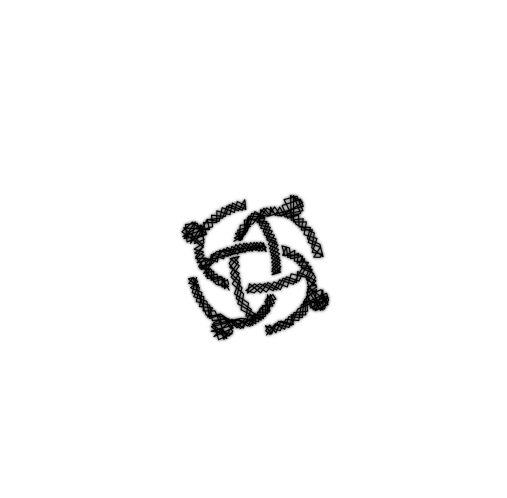
\includegraphics[width=\linewidth,
                     height=0.8\textheight,
                     keepaspectratio]{linuxdev-br}
  \end{figure}
\end{frame}

\begin{frame}{S2 Linuxdev-br}
  \begin{figure}
    \centering
    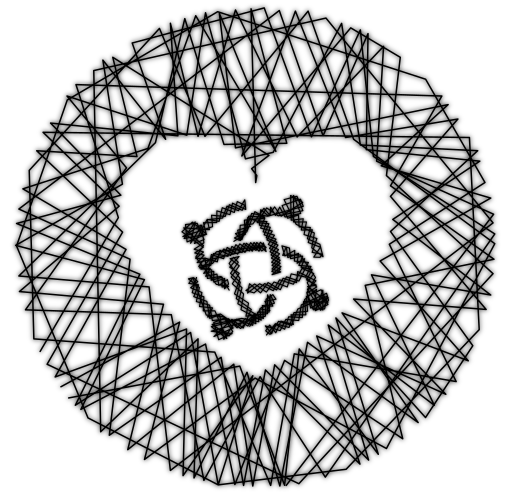
\includegraphics[width=\linewidth,
                     height=0.8\textheight,
                     keepaspectratio]{love_linuxdev-br}
  \end{figure}
\end{frame}

%------------------------------------------------------------------------------
\section{About this presentation}
\begin{frame}[standout]
   \begin{center}\ccbysa\end{center}
\end{frame}

\maketitle

\end{document}
